% !TEX root = arbeit.tex
\section{Experiments} \label{sec:Exp}
	
	This section includes tests of flight components and also system tests of the NIM Proto Flight Model (PFM) and the Flight Spare (FS) model. The tests of the flight ion-mirror and the flight antechamber were performed with the NIM Prototype whereas the other tests were performed with the NIM PFM model unless otherwise mentioned.

%-----------------------------------------------------------------------------------
	\subsection{Flight Ion-Mirror}
	In this section the performance of two ion-mirrors is compared. As described in Chapter~\ref{sec:setup}, the prototype ion-mirror consists of several ring-electrodes connected with each other with resistors to generate a linear voltage gradient. The flight ion-mirror consists of a ceramic tube with two resistance spirals replacing some of the ring-electrodes. Fig.~\ref{fig:ExpRefl}~left shows the prototype ion-mirror and Fig.~\ref{fig:ExpRefl}~right shows the flight ion-mirror mounted to the NIM prototype in the test setup. An ion-mirror of the same type as the flight ion-mirror was also used in the RTOF mass spectrometer, which flew in the ROSINA \cite{Diss_Scherer} and in the NGMS instrument \cite{Diss_Hofer}. From the electrical point of view, the two ion-mirror types behave the same.\\
	The measurements were performed in a vacuum chamber. The residual gas pressure for the measurements with the prototype ion-mirror was 5$\cdot$10\textsuperscript{-10}~mbar and for the measurements with the flight ion-mirror 1.4$\cdot$10\textsuperscript{-9}~mbar. The test gases were injected directly through a leak valve to increase the chamber pressure up to 1$\cdot$10\textsuperscript{-8}~mbar. The used test gases were: Ne, Ar, Kr and Xe. 3~Mio. single spectra were histogramed for each of the measurements. All voltages of the instrument were manually optimised for the measurements with the two ion-mirrors. Table~\ref{tab:refPerftab} shows the signal-to-noise ratios and the mass resolution of the different test gases measured with the two instrument configurations.\\
	The SNR of the measurements with the flight ion-mirror is for all gases lower than the SNR of the measurements with the prototype ion-mirror, the mass resolution of the flight ion-mirror is slightly better than with the prototype ion-mirror. The better SNR performance of the prototype ion-mirror is due the much longer calibration time, and thus better optimisation of
	\begin{figure}[H]
		\begin{subfigure}{0.5\textwidth}
			\centering
			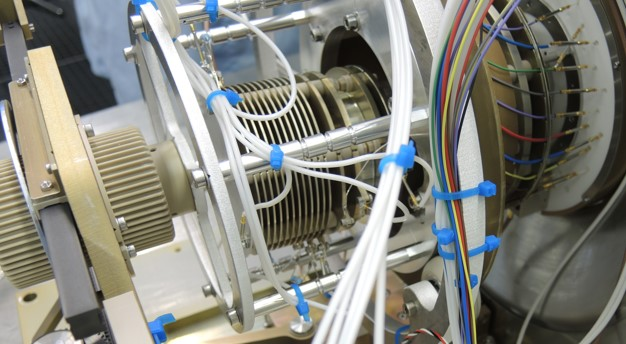
\includegraphics[width = 0.95\textwidth]{Experiments/reflectron_Prototype1.jpg}
		\end{subfigure}
		\begin{subfigure}{0.5\textwidth}
			\centering
			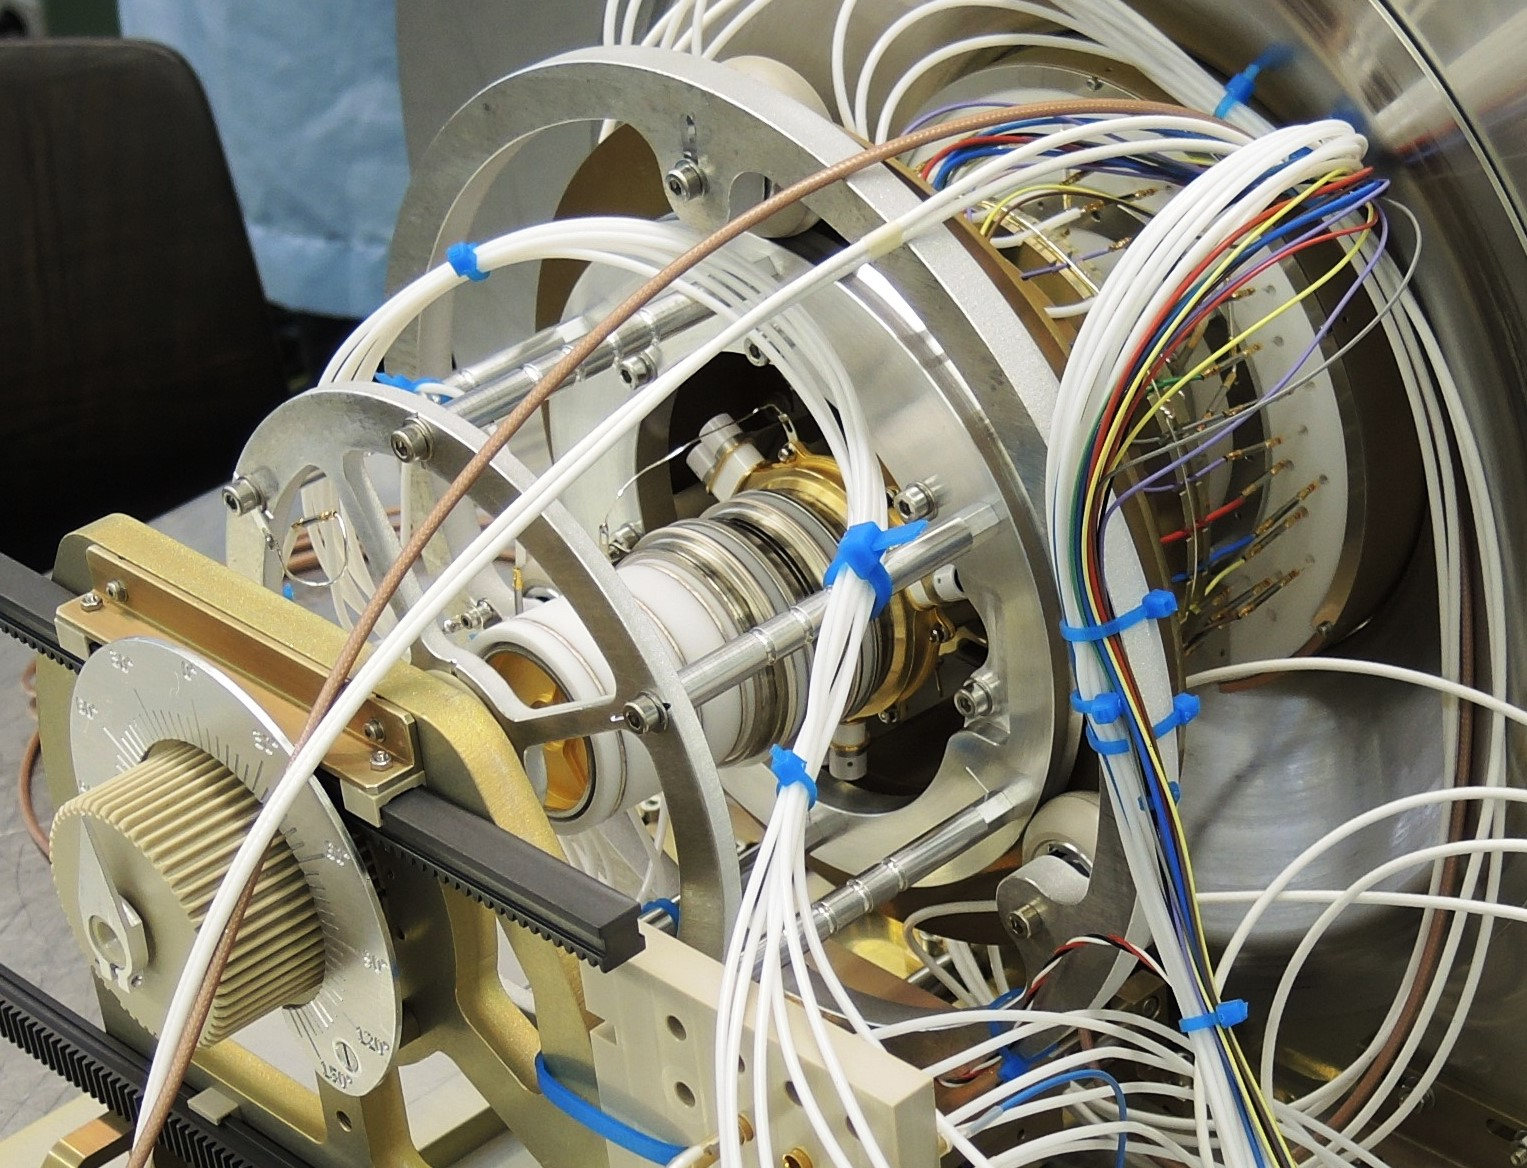
\includegraphics[width = 0.85\textwidth]{Experiments/reflectron_flight.JPG}
		\end{subfigure}
		\caption{Prototype ion-optical system with prototype ion-mirror with ring-electrodes (left panel) and flight ion-mirror attached (right panel).}
		\label{fig:ExpRefl}
	\end{figure}
	\begin{table}[H]
		\begin{center}
		\begin{tabular}{|l|r|r|r|r|}
			\hline
			Gas						&SNR ProtoR	&SNR PFMR	&m/$\Delta$m ProtoR	&m/$\Delta$m PFMR\\
			\hline
			\textsuperscript{20}Ne	&2022.9		&562.4		&200 ± 12		&236 ± 16\\
			\textsuperscript{40}Ar	&4732.6		&1808.4		&212 ±  9		&267 ± 15\\
			\textsuperscript{86}Kr	&746.1		&414.3		&224 ±  7		&292 ± 12\\
			\textsuperscript{136}Xe	&185.5		&97.1		&265 ±  8		&332 ± 13\\
			\hline
		\end{tabular}
		\end{center}
		\caption{Table listing the signal-to-noise ratios (SNR) and the mass resolution (m/$\Delta$m) of the prototype ion-mirror (ProtoR) and the flight ion-mirror (PFMR).}
		\label{tab:refPerftab}
	\end{table}
	the ion-optical system, of the Prototype with the prototype ion-mirror. To set constrains for the different subsystems of the NIM ion-optical system, a whole calibration campaign was performed with the prototype ion-mirror attached \cite{Diss_Meyer}. Therefore, this configuration is much better optimised than the configuration where the flight ion-mirror is attached to the Prototype ion-optical system. Nevertheless, the flight ion-mirror showed good performance considering the short optimisation time available to verify its performance.
	
	
%----------------------------------------------------------------------------------
	\subsection{Flight Antechamber} \label{subsec:ExpAnteCham}
	% dimensions old antechamber: d_in = 4 mm, d_out = 3 mm, d_sp = 40 mm
	%			 new:			  d_in = 5 mm, d_out = 4 mm, d_sp = 80 mm
	% For further explanation of the geometry see Chap.\ref{subsubsec:Densenhan}.
	After successfully testing the flight ion-mirror, the flight antechamber was tested. A picture of the prototype and the flight antechamber is shown in Fig.~\ref{fig:expAntchamPic}. The antechambers consist of two parts. In the old design the two parts of the antechamber had a rim on which the screws were mounted to put the two parts together. These screws were at position $\pm$45°. Tests with this antechamber revealed that neutral particles hit these screws and scatter into chamber (Fig.~\ref{fig:AnteMeasData}~a) \cite{Meyer_2017_ante}). Therefore, an antechamber with a flat outer surface was required. In the new design the screws are recessed into the 1~mm thin surface of the antechamber to get rid of the needed rim in the old design. In addition, the new antechamber is by a factor two bigger than the prototype antechamber with the aim to get more signal. Simulations of the flight trajectory revealed that two holes were required at positions $\pm$60° to get optimal signal \cite{SOC_Crema3p2}. The CASYMIR test facility is not able to direct the neutral particle beam under an angle of 60° onto the instrument. To test the new design, an slightly different antechamber was used with the second entrance hole at position $\theta_0 = -90\degree$ instead of --60°. With a rotation mechanism, the instrument can be rotated around the x-axes by $\pm$90°.\\
	\begin{figure}[h!]
		\begin{subfigure}{.5\textwidth}
			\centering
			\includegraphics[width=\textwidth]{Experiments/ProtoAnte.png}
		\end{subfigure}
		\begin{subfigure}{.5\textwidth}
			\centering
			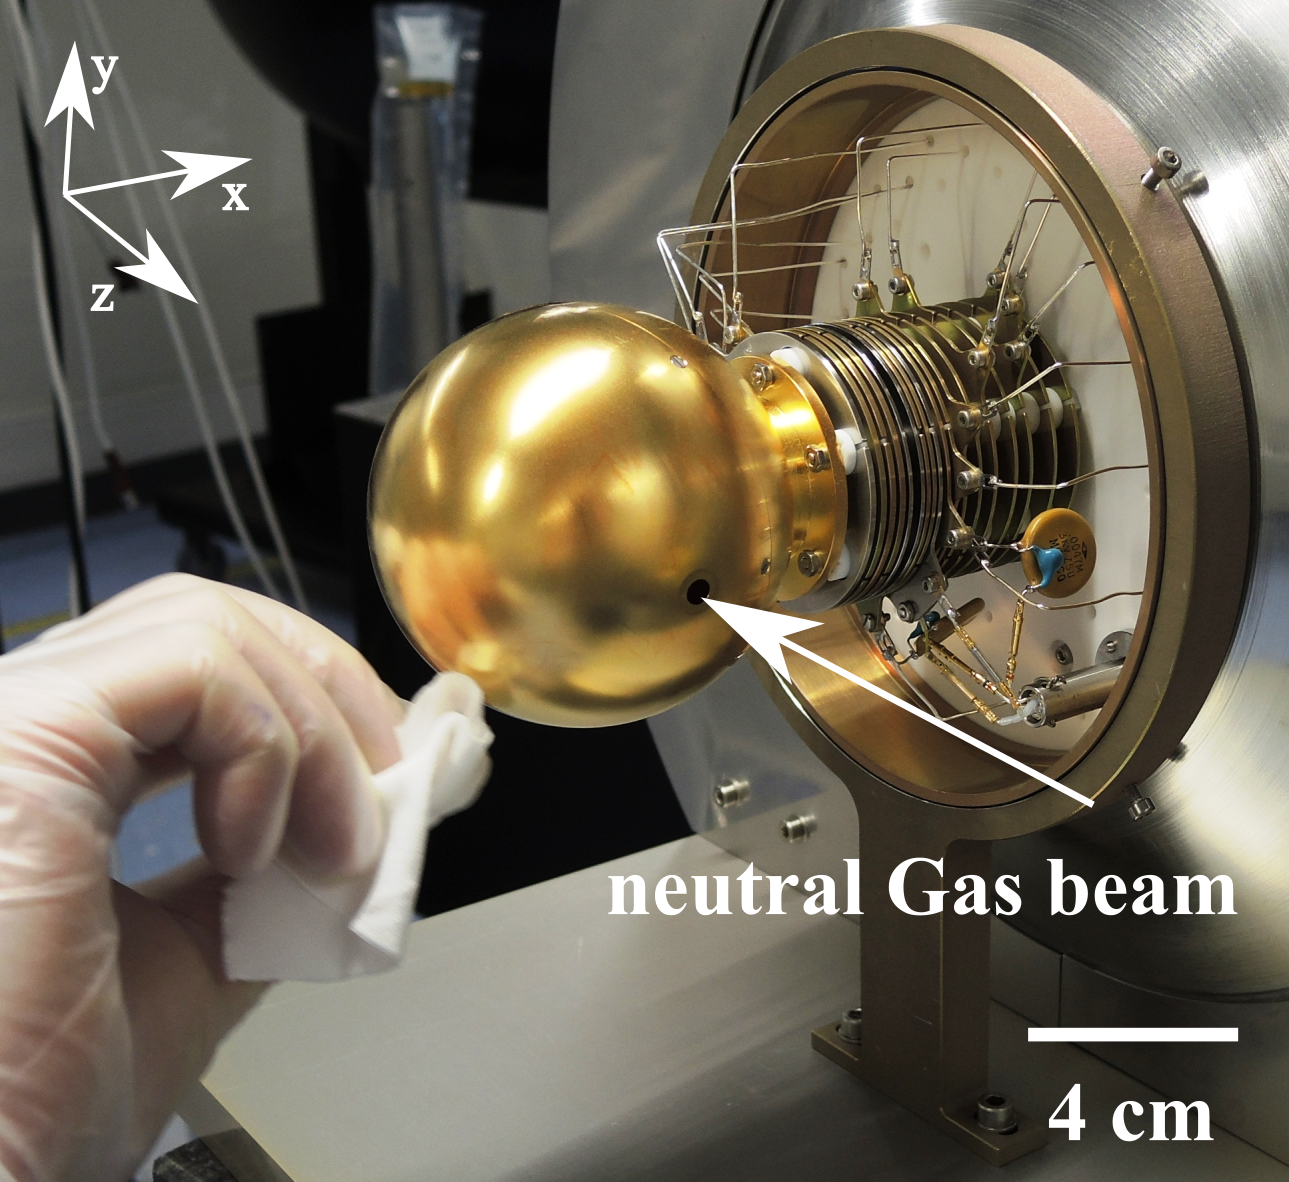
\includegraphics[width=.8\textwidth]{Experiments/FlightAnte.png}
		\end{subfigure}
		\caption{Left: Prototype antechamber. Right: flight-like antechamber with two entrance holes at positions +60° and --90°.}
		\label{fig:expAntchamPic}
	\end{figure}
	These measurements were conducted at the CASYMIR test facility at the University of Bern. CASYMIR is able to generate a neutral particle beam with velocities up to 5.5~km/s \cite{CASYMIR_Graf2004}. For these measurements the particle velocity was about 2.5~km/s because this is the velocity of the spacecraft in Ganymede orbit, which will be 90\% of the measuring time of NIM.\\
	\begin{figure}[h!]
		\begin{subfigure}[t]{.5\textwidth}
			\centering
			\includegraphics[width=\textwidth]{Experiments/oldAnte_ThMode.png}
			\caption{Prototype antechamber, thermal mode.}
		\end{subfigure}
		\begin{subfigure}[t]{.5\textwidth}
			\centering
			\includegraphics[width=\textwidth]{Experiments/oldAnte_NMode.png}
			\caption{Prototype antechamber, neutral mode.}
		\end{subfigure}
		\begin{subfigure}[b]{.5\textwidth}
			\centering
			\includegraphics[width=\textwidth]{Experiments/newAnte_ThMode.png}
			\caption{Flight-like antechamber, thermal mode.}
		\end{subfigure}
		\begin{subfigure}[b]{.5\textwidth}
			\centering
			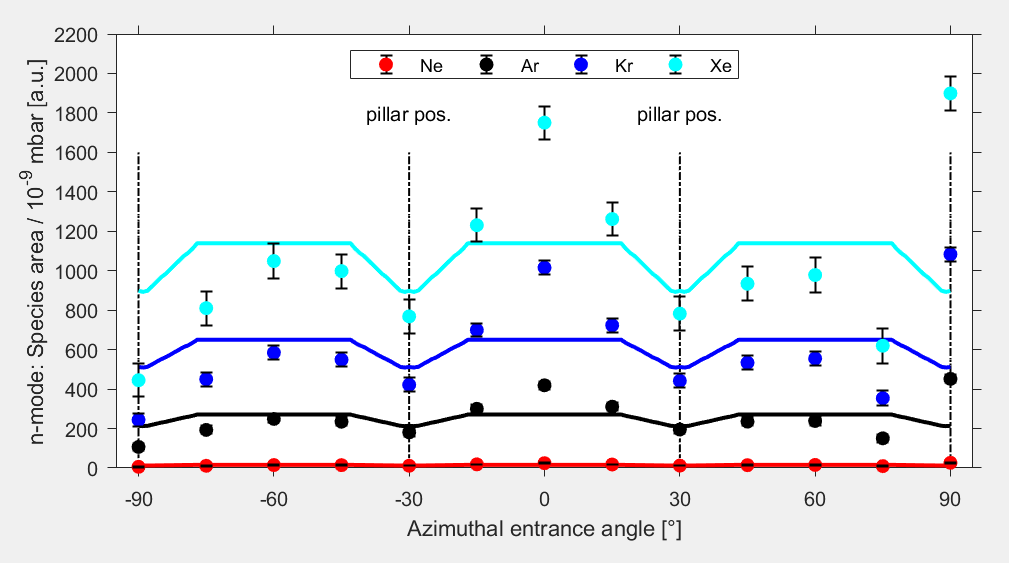
\includegraphics[width=\textwidth]{Experiments/newAnte_NMode.png}
			\caption{Flight-like antechamber, neutral mode.}
		\end{subfigure}
		\caption{Panel a) an b) show measurements done with the NIM Prototype ion-optical system with the old antechamber attached. a) shows measurement conducted with the thermal gas mode and panel b) shows measurements of the neutral mode respectively \cite{Meyer_2017_ante}. c) and d) are the corresponding measurements performed with the new antechamber attached to the NIM Prototype.}
		\label{fig:AnteMeasData}
	\end{figure}
	Fig.~\ref{fig:AnteMeasData}~a) shows measurements conducted with the thermal mode when the old antechamber was attached \cite{Meyer_2017_ante}. For these measurements, the instrument was rotated around the x-axis by keeping the beam at the same position. When rotating the antechamber, the hole moves out of the neutral particle beam because the beam is smaller than the antechamber. The expected intensity distribution $I_{ant}$ is a combination of the function of the moving hole through the beam with a normal distribution:
	\begin{equation}
		I_{ant} = \frac{A}{\sigma\sqrt{2\pi}}\int_{x_{min}}^{x_{max}} \exp^{\frac{(x-\mu)^2}{2\sigma^2}} dx
		\label{eq:IantProto}
	\end{equation}
	With $A$ a constant taking the beam intensity into account, $\sigma$ the standard deviation of the beam and $\mu$ the position of the beam centre relative to the centre of the antechamber, which is zero in this coordinate system. The borders of the integral (Eq.~\eqref{eq:IantProto}) determine the section of the beam entering the antechamber:
	\begin{align}
		x_{max} &= r_{ant}\sin{\alpha} - r_{aHi}\cos{\alpha}\label{eq:antIntgrLimHigh}\\
		x_{min} &= r_{ant}\sin{\alpha} + r_{aHi}\cos{\alpha}\label{eq:antIntgrLimLow}
	\end{align}
	With $r_{ant}$ the radius of the antechamber and $r_{aHi}$ the radius of the antechamber entrance hole. The sine contribution considers the shift of the hole in y-direction when the hole is rotated. The cosine contribution originates from the projection of the beam on the entrance hole. For the measurements with the new antechamber, the shift in y-direction when rotating the instrument was compensated by shifting the whole instrument. Therefore the sine contribution in Eq.~\eqref{eq:antIntgrLimHigh} and Eq.~\eqref{eq:antIntgrLimLow} cancels leading to a cosine-like function.\\
	When comparing Fig.~\ref{fig:AnteMeasData}~a) and c), the artefacts successfully vanished after the redesign. The higher intensity at angle +90° is an outlier because it appears in both the thermal (Fig.~\ref{fig:AnteMeasData}~b)) and the neutral mode figure (Fig.~\ref{fig:AnteMeasData}~d)) of the measurements with the new antechamber. The lower measured signal intensity for the measurements with the new antechamber is a result of having an additional entrance hole which was necessary because of the flyby trajectories (see Chap.~\ref{subsubsec:Densenhan}).\\
	Fig.~\ref{fig:AnteMeasData}~b) shows measurements conducted with the neutral gas mode with the old antechamber attached and Fig.~\ref{fig:AnteMeasData}~d) shows measurements conducted with the neutral gas mode when the new antechamber was attached. At position $\pm$30° and $\pm$90° are pillars holding the stack of the ion-optical lenses together. When the beam hits these pillars, the particles scatter in all directions leading to a reduction of the signal. For the neutral gas channel, no difference in the signal distribution and intensity is expected because a change in the antechamber design does not influence the signal measured with the neutral gas channel. The observed signal of the neutral gas mode when the new antechamber is attached, is significantly higher than with the old antechamber. This is due to a better voltage set. A different voltage set for the voltages in the ionisation region changes the distribution of the electron beam thus leading to a different ion distribution in the ionisation region. This leads to a different angular distribution of the signal for the neutral gas channel when comparing the results of the two measurement series. 
	
%---------------------------------------------------------------------------------------------------
	\subsection{Density Enhancement}\label{chap:expDensEntSlit}
	For the first tests with the NIM PFM, the front side of the NIM instrument was scanned with the neutral particle beam to find the position of the entrance slit and the antechamber entrance hole to align the beam properly with the instrument. Fig.~\ref{exp:PFMIntCharTot}, left panel shows the scan of the front side and Fig.~\ref{exp:PFMIntCharTot}, right panel shows the corresponding structural part. The antechamber entrance hole is clearly visible as a small dot. Fig.~\ref{exp:PFMIntCharAnt} shows a zoom with a better resolution of the antechamber entrance hole which shows a nice Gaussian distribution. When looking at the entrance slit, there are two positions with increased intensities. The zoom on Fig.~\ref{exp:PFMIntCharEnt} reveals that the positions of biggest intensity is were the beam hits the structure covering the two electron emitting filaments. The other intensity maximum is where the beam hits the supporting structure opposite of the filament bloc. When the gas hits these structures, the gas slows down leading to a local increase of the gas density. Therefore, the structure partially thermalises the gas similar as the closed source antechamber. This was not intended because with the neutral gas channel the aim is to measure incoming neutral particles and ions directly without any interaction with the structure. In the design of the PFM, the filament bloc and the supporting structure act like a funnel directing the scattered gas to the central grid. The thermalisation of the incoming gas when it hits the filament bloc is unavoidable. For the supporting structure opposite of the filament, a pillar instead of the plate like structure would have been the better option. When the gas hits the pillar, the pillar scatters the gas in all directions instead of scattering only in the direction of the central grid. This phenomenon was observed when doing a similar measurement with the NIM prototype (Fig.~\ref{exp:ProtoIntCharEnt}).\\
	\begin{figure}[H]
		\centering
		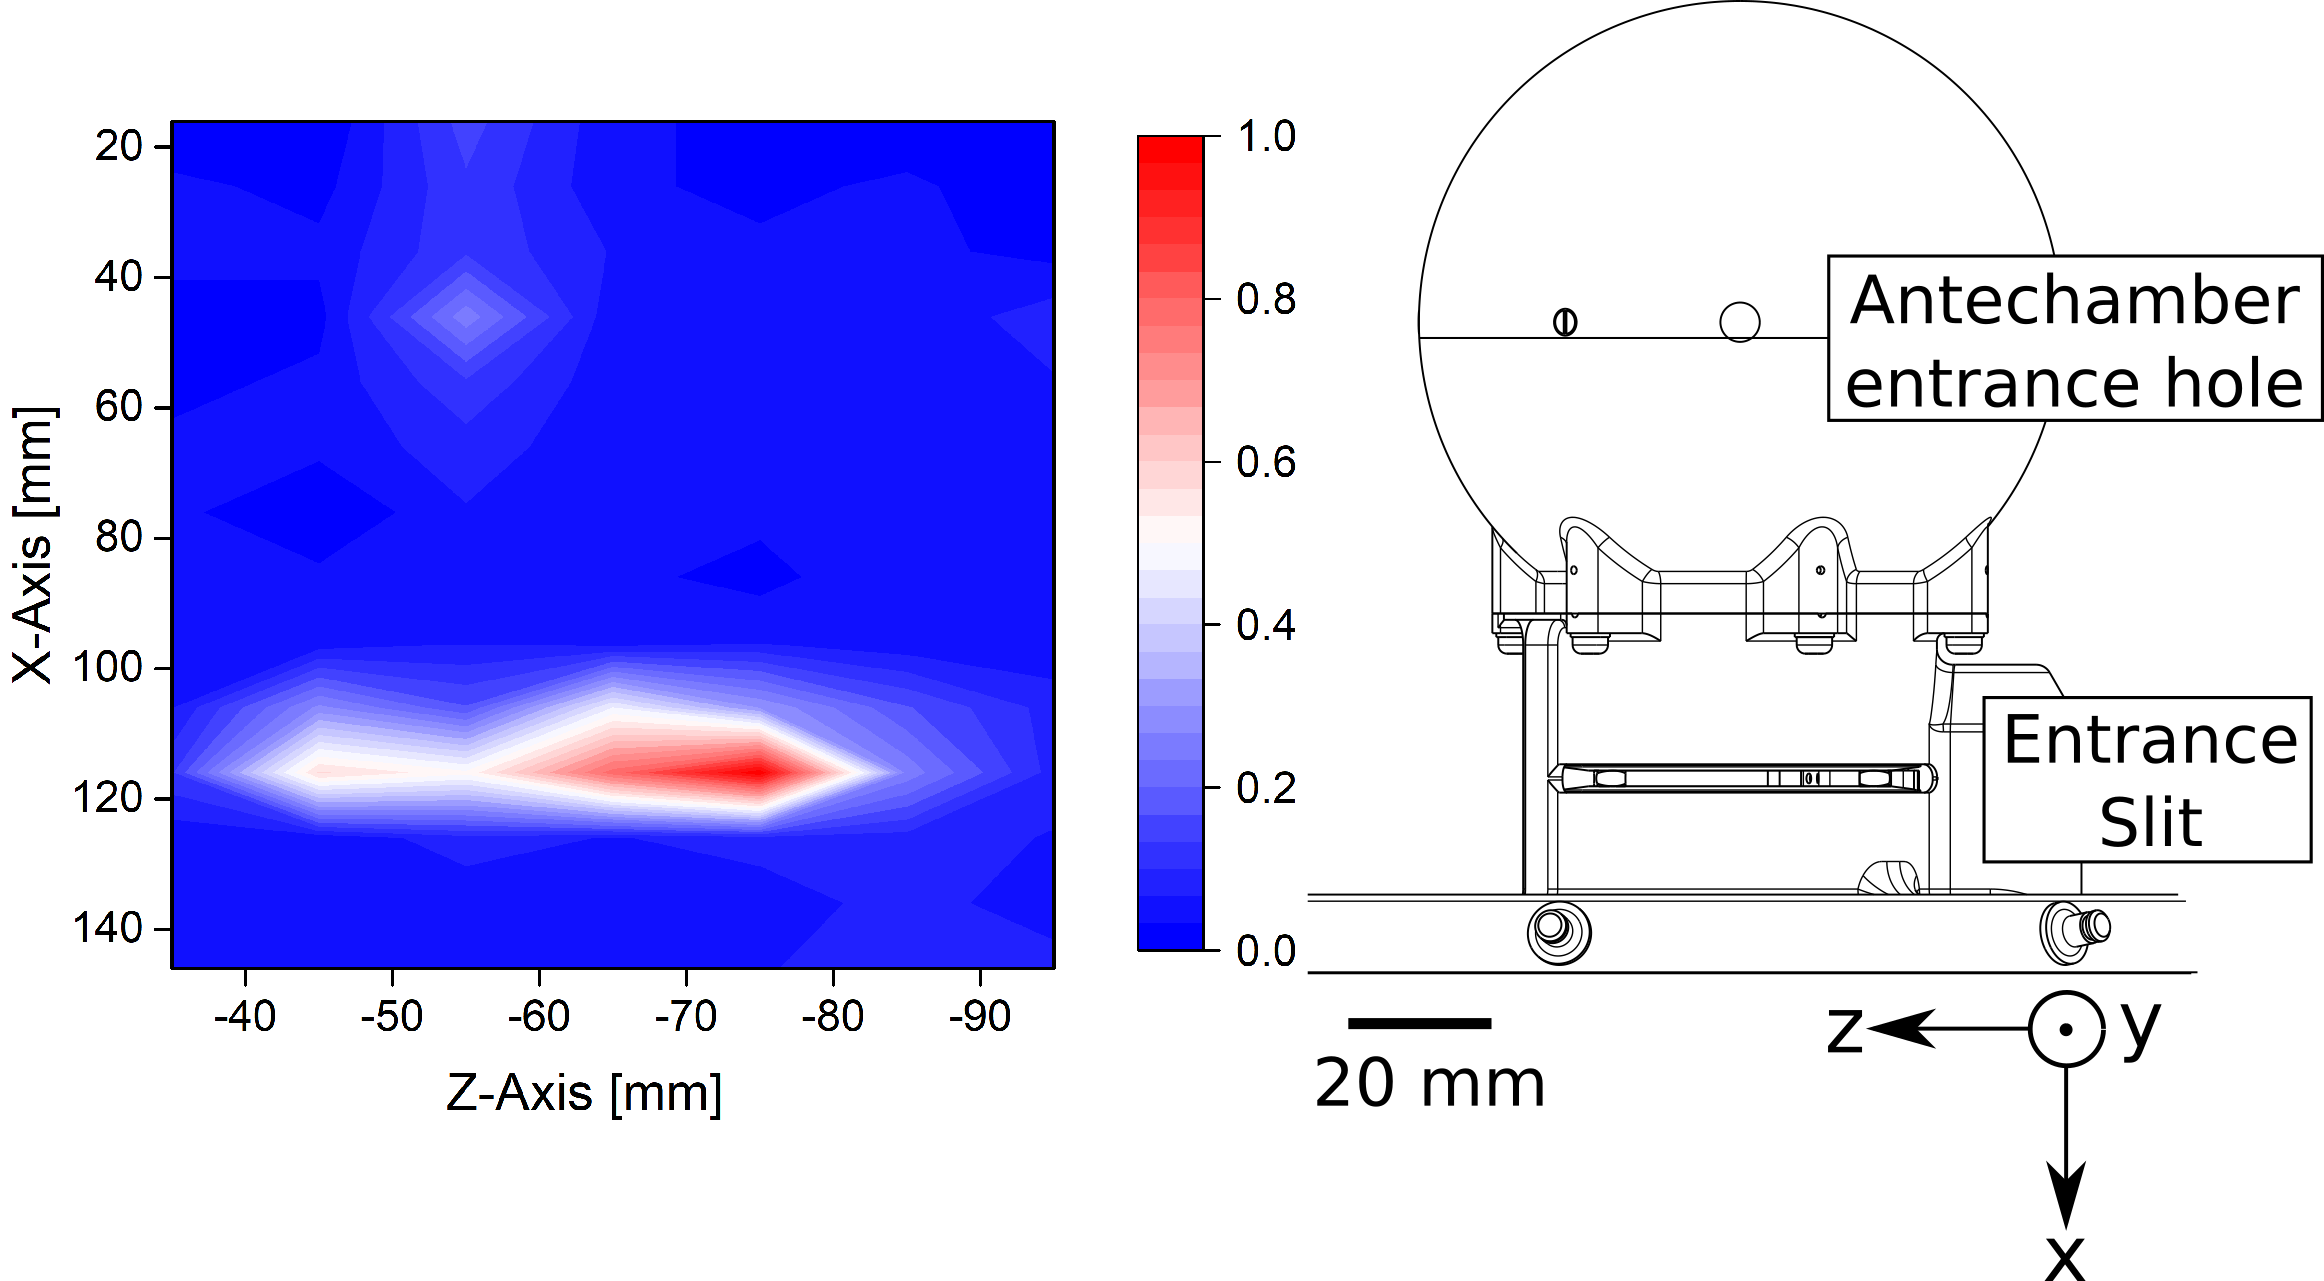
\includegraphics[width=\textwidth]{Experiments/2D_scan_anteEntr.png}
		\caption{Left: Intensity profile when directing the neutral particle beam at the structure of the NIM PFM instrument. Right: Front view as seen by the neutral particle beam.}
		\label{exp:PFMIntCharTot}
	\end{figure}
	\begin{figure}[h!]
		\centering
		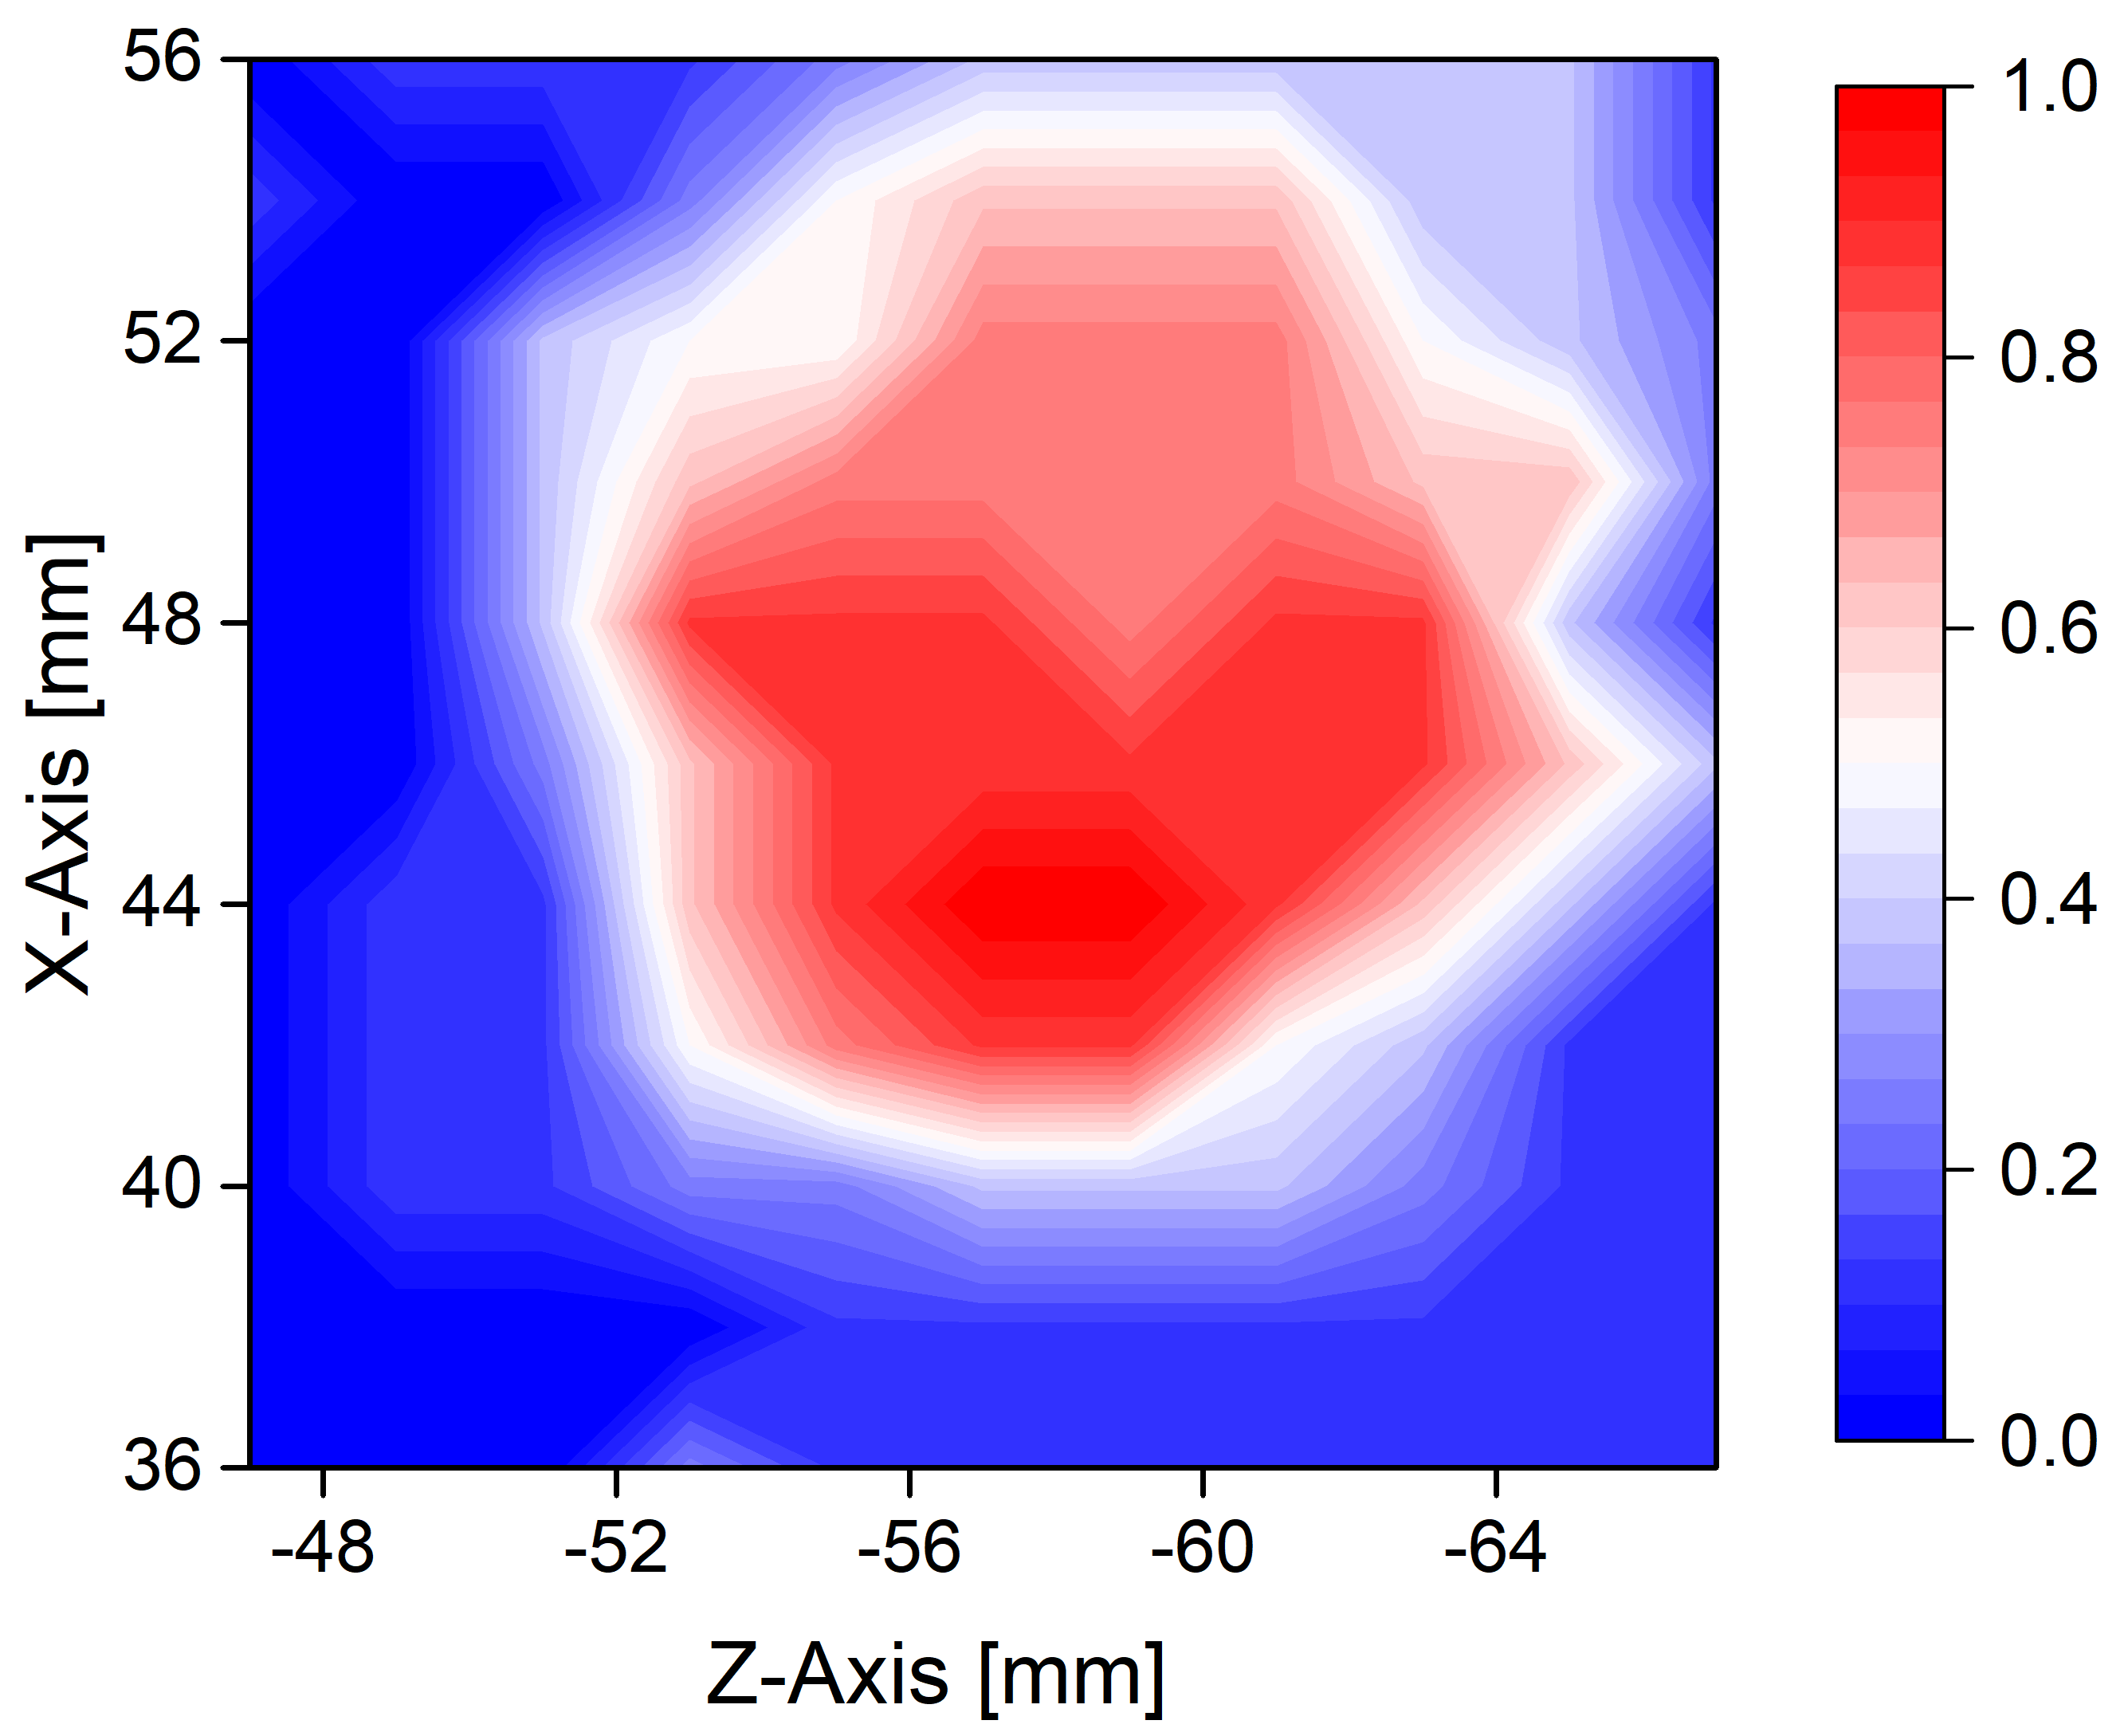
\includegraphics[width=.6\textwidth]{Experiments/2D_scan_Ant.png}
		\caption{Detail on the antechamber hole when directing the neutral particle beam at the structure of the NIM PFM instrument. Note that the intensity scale is different to Fig.~\ref{exp:PFMIntCharTot}}
		\label{exp:PFMIntCharAnt}
	\end{figure}	
	\begin{figure}[h!]
		\centering
		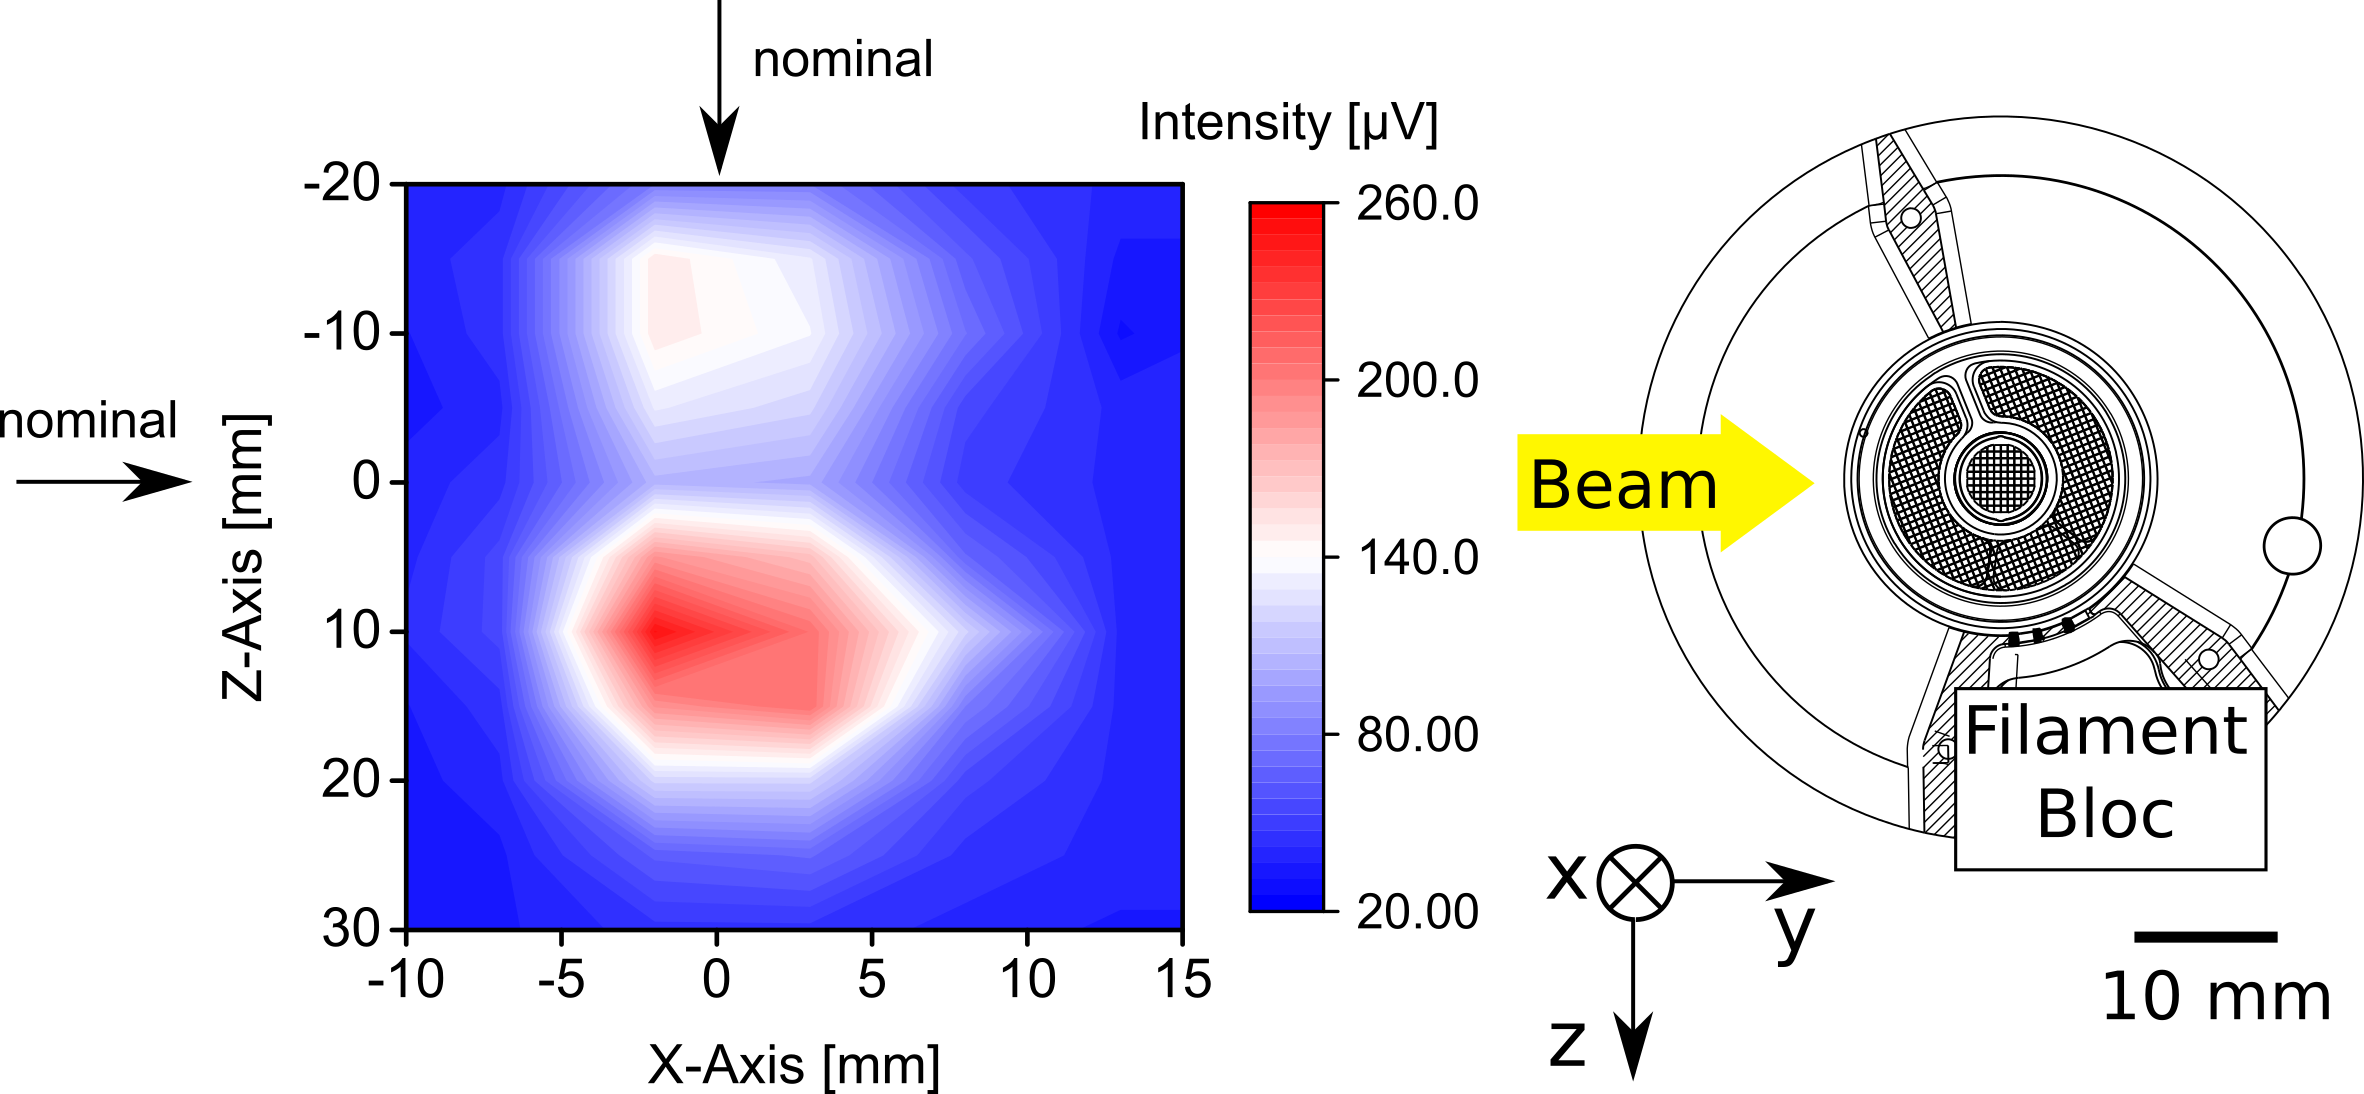
\includegraphics[width=\textwidth]{Experiments/2D_scan_Entr.png}
		\caption{Left: Detail of the scan of the front side of NIM with the neutral particle beam (Fig.~\ref{exp:PFMIntCharTot} right). Right: Top view on the ionisation region.}
		\label{exp:PFMIntCharEnt}
	\end{figure}
	\pagebreak
	The ion-source of the prototype had six pillars holding the different focusing lenses together. In Fig.~\ref{exp:ProtoIntCharEnt} the pillars are marked as red circles. The electron emitting filament was opposite of the main gas inflow direction. For these measurements, the ionisation region was scanned with the neutral particle beam at angles 0° and $\pm$60° to direct the beam in between the pillars over the extraction grid. When scanning from the front side, the signal intensity has a nice Gaussian shape. When scanning the ionisation region at angles of $\pm$60° the Gaussian distribution is visible when the neutral particle beam is aligned over the centre grid with an asymmetry toward the side of the filament bloc. The gas hitting the filament bloc gets thermalised leading to a higher signal than on the other side of the were the gas only scatters on the pillars. Here the signal increase due to thermalisation is less dominant than in the design of the PFM because the part of the filament structure seen by the beam is tilted outward. At distances bigger than $\pm$25~mm from the centre, the signal drops again. This is where the beam is completely outside of the ionisation region.
	\begin{figure}[h!]
		\centering
		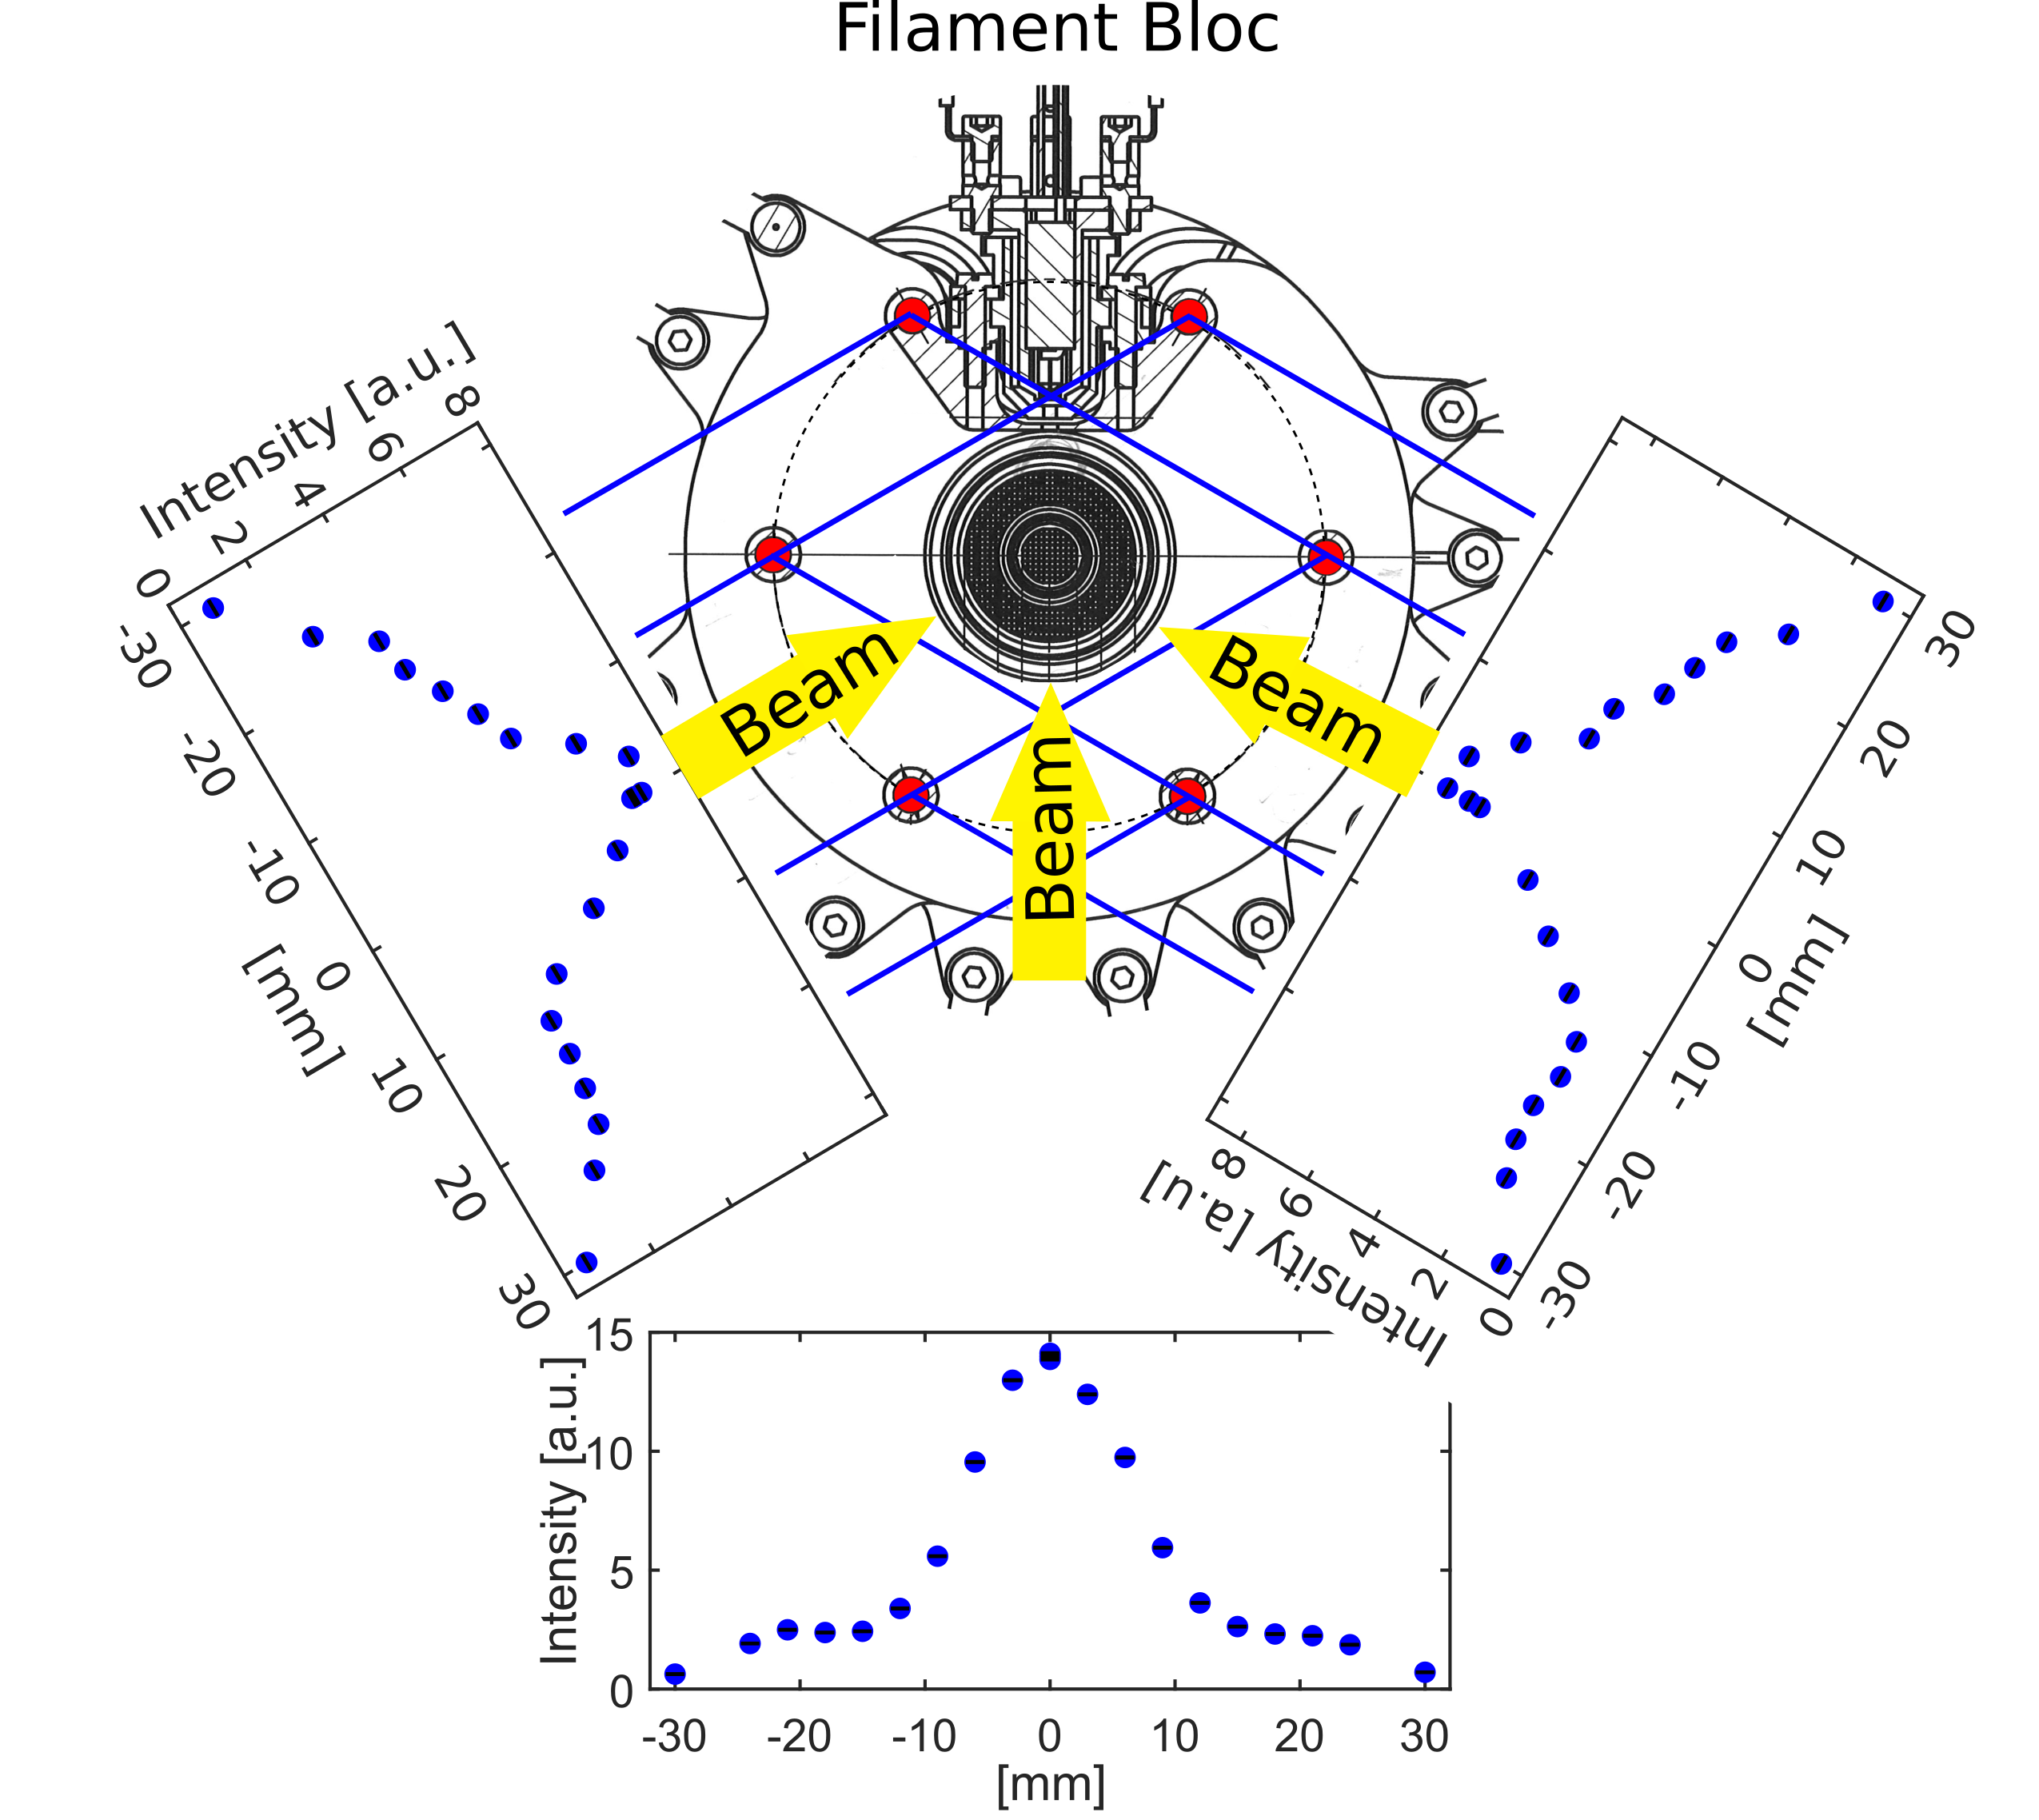
\includegraphics[width=\textwidth]{Experiments/Entrence_Proto_topview.png}
		\caption{Detail on the entrance seen from above the entrance plane when directing the neutral particle beam at the structure of the NIM Prototype. The red circles mark the positions of the pillars holding the ion source together.}
		\label{exp:ProtoIntCharEnt}
	\end{figure}
	
	
%-----------------------------------------------------------------------------------
	\subsection{Entrance Ion and Electron Position Simulations}
	This chapter shows at which start positions the ions in the ionisation region have to be to successfully reach the detector when the extraction pulse is applied on the extraction grid. In addition, this chapter includes simulations of the flight path of the electron beam which is used to ionise the neutral particles.\\
	Fig.~\ref{fig:PFMentrSideTopSchemas}, top panel shows the ionisation region from the side. The pink tube opposite of IS~5 is the tube connecting the antechamber with the ionisation region. Neutral particles are ionised with an electron beam (blue arrow) and pulled into the analyser section with the inner extraction grid IS~5 (th-Mode and n-Mode). Ions penetrating the ionisation region are pulled with the outer extraction grid IS~6 into the analyser section (i-Mode). Fig.~\ref{fig:PFMentrSideTopSchemas}~bottom shows the top view of the ionisation region when looking from the antechamber. On the right side are the two filaments used to generate the ionising electron beam and on the left side is a supporting structure to support the antechamber from the other side. In n-Mode and i-Mode, the gas 
	\begin{figure}[h] % Entrance schema.
		\begin{subfigure}[t]{\textwidth}
			\centering
			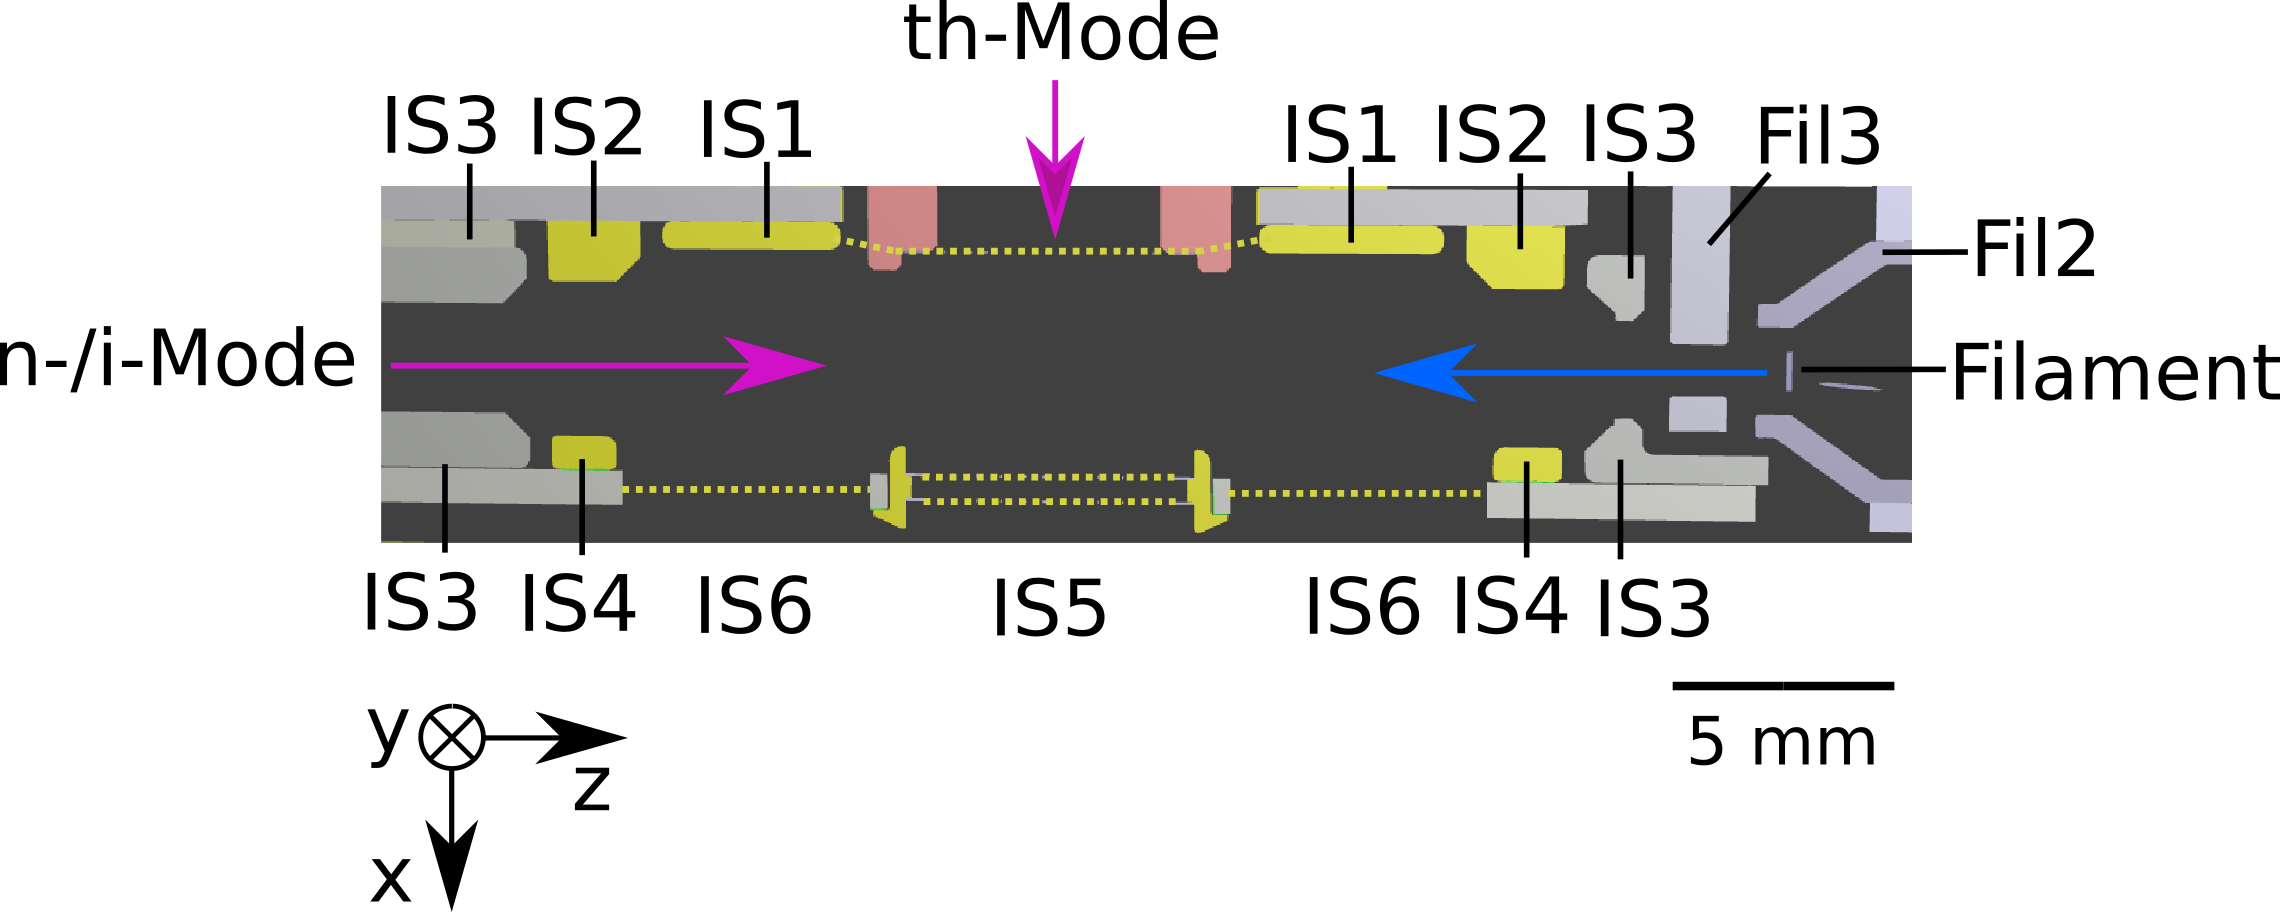
\includegraphics[width=.8\textwidth]{Experiments/PFMEntrance_Side_Schema.png}
			%	\caption{Side view.}
		\end{subfigure}
		\par\bigskip
		\begin{subfigure}[b]{\textwidth}
			\centering
			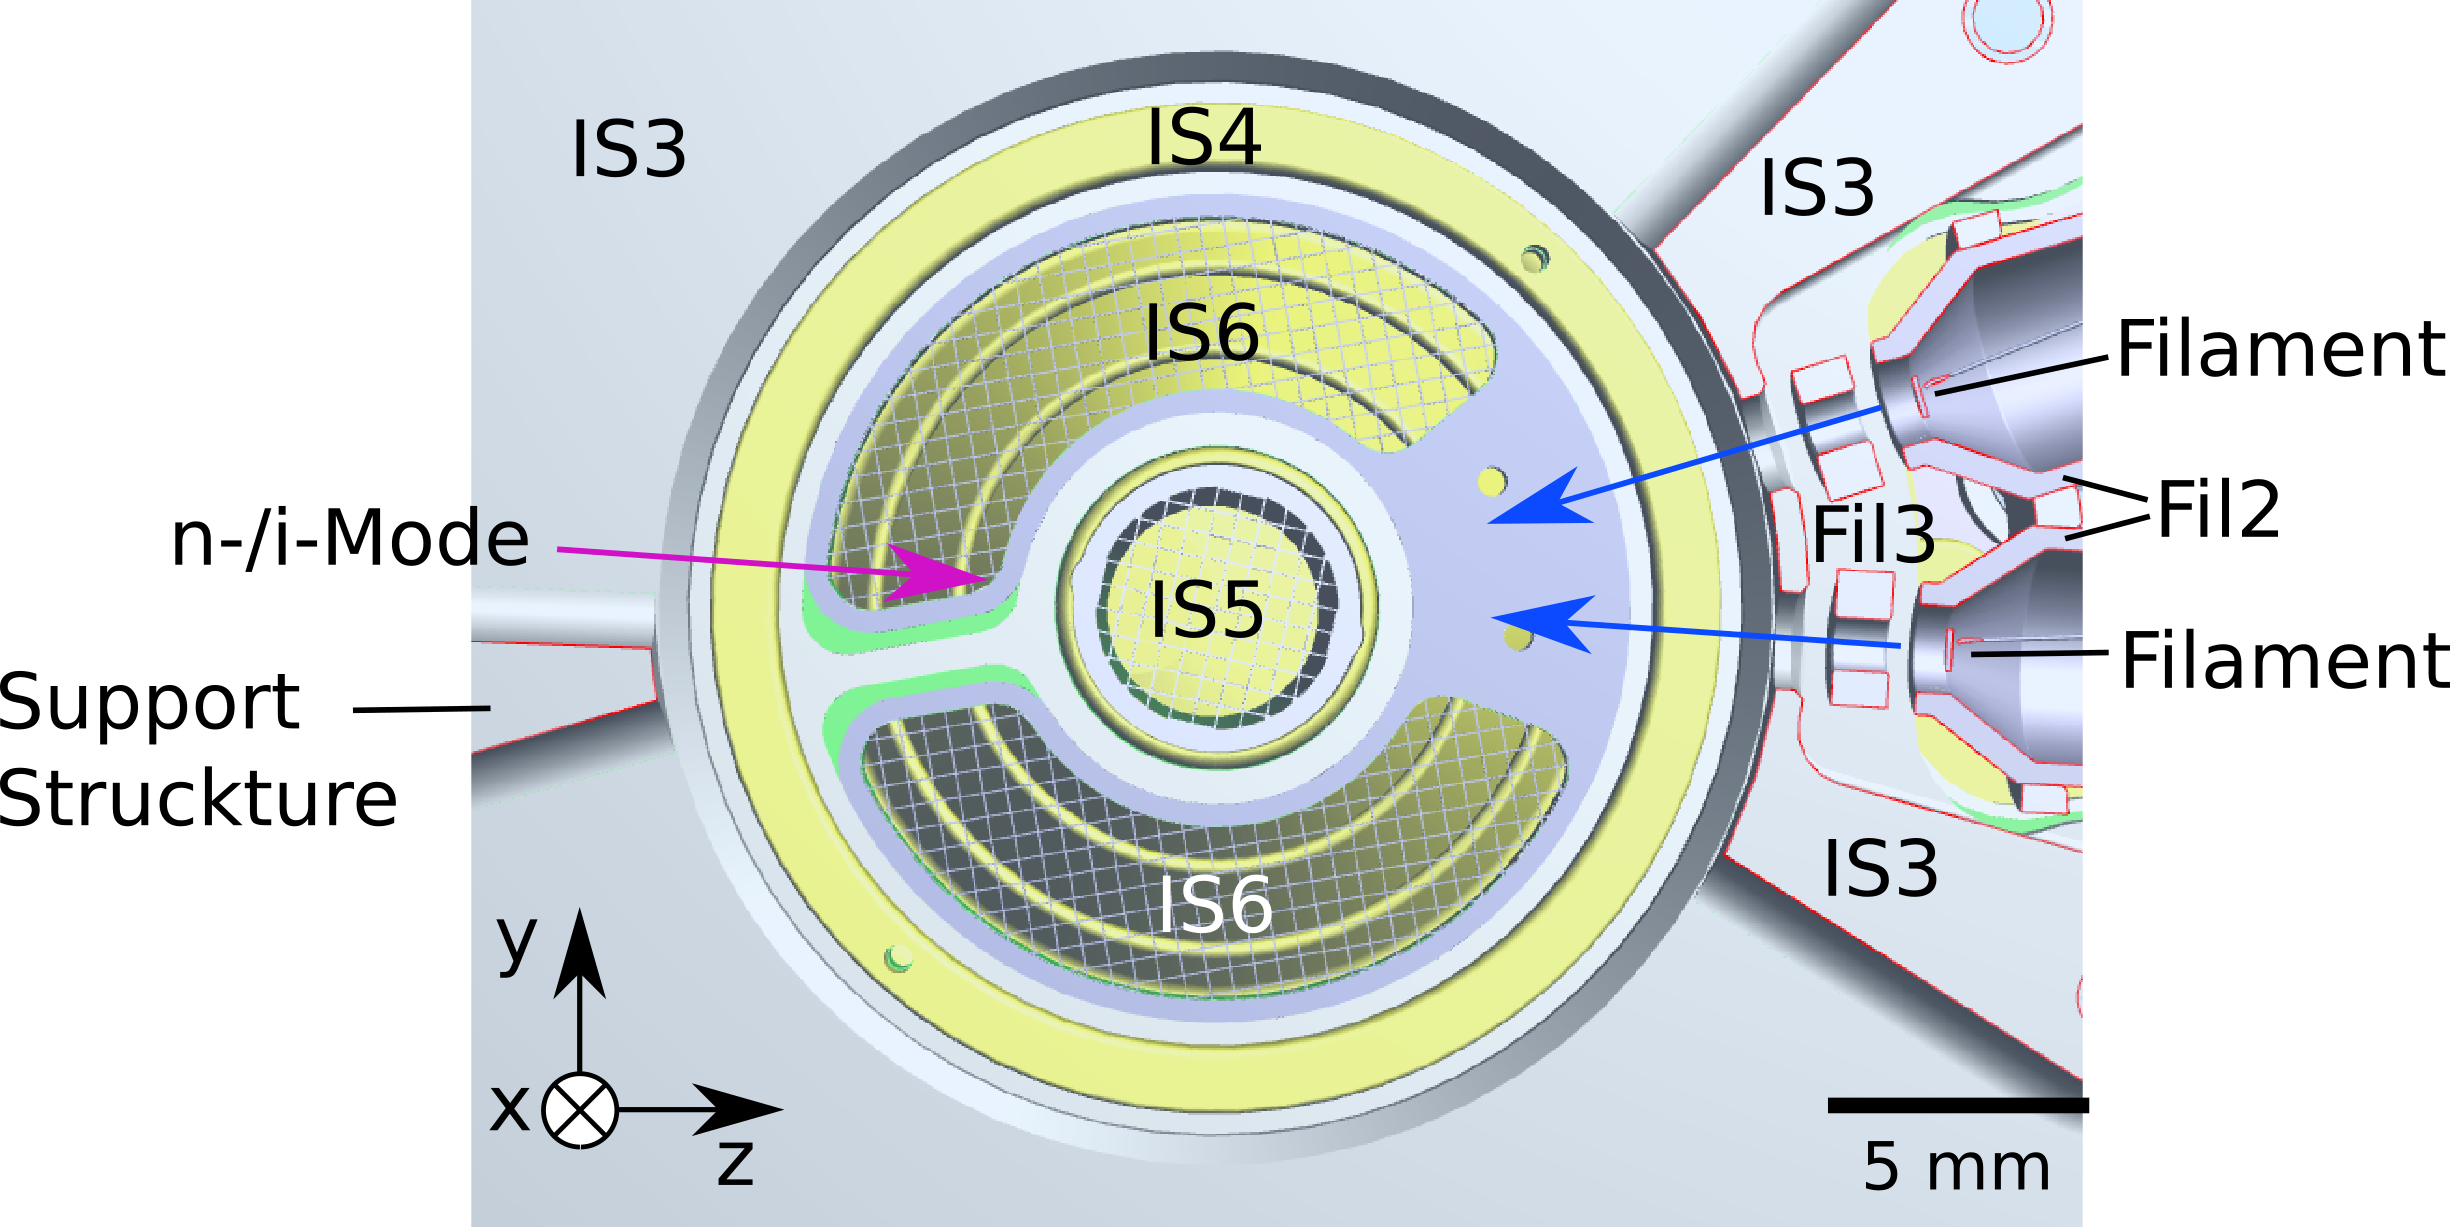
\includegraphics[width=.85\textwidth]{Experiments/PFMEntrance_Top_Schema.png}
			%	\caption{Top view}
		\end{subfigure}
		\caption{Side (top) and top view (bottom) of the ionisation region. The violet arrows mark the gas inflow direction and the blue arrows mark the direction of the electron beam.}
		\label{fig:PFMentrSideTopSchemas}
	\end{figure}
	\begin{figure}[h] % Sim ions reach the detector th- & n-Mode.
		\begin{subfigure}[t]{.5\textwidth}
			\centering
			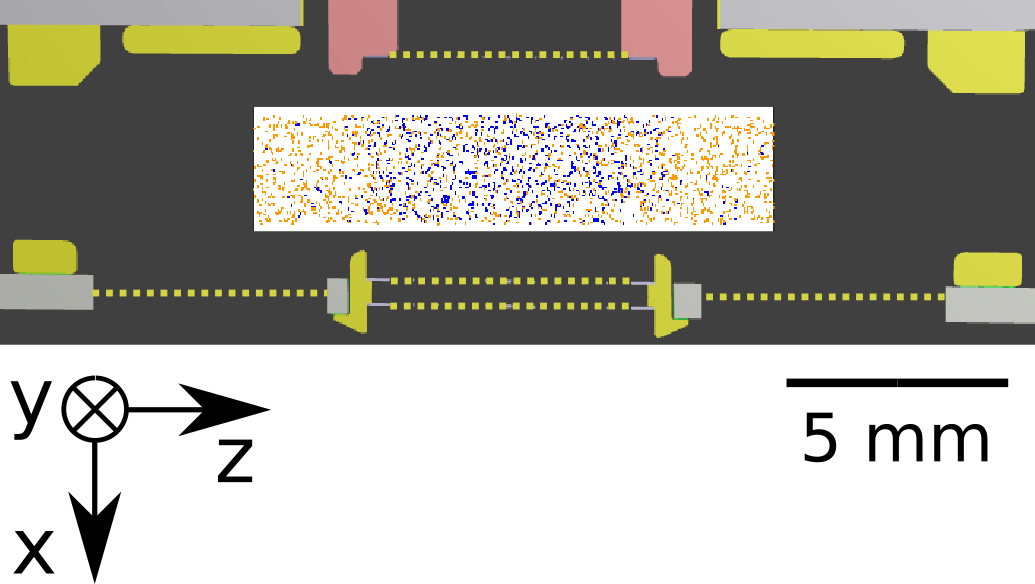
\includegraphics[width=.8\textwidth]{Experiments/PFMEntrance_Side_thSim.png}
			\caption{Side view, thermal mode.}
		\end{subfigure}
		\begin{subfigure}[t]{.5\textwidth}
			\centering
			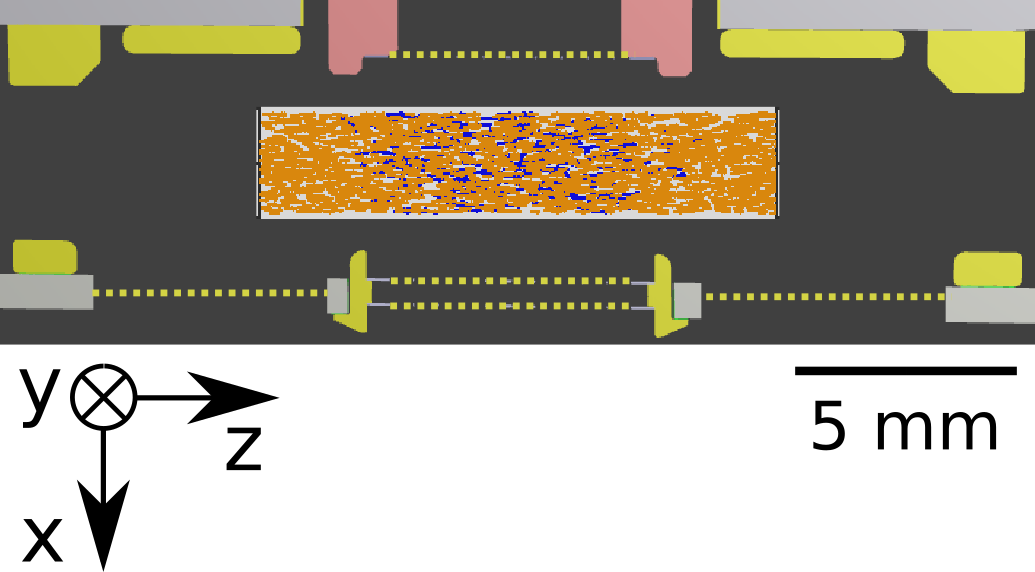
\includegraphics[width=.8\textwidth]{Experiments/PFMEntrance_Side_nSim.png}
			\caption{Side view, neutral mode.}
		\end{subfigure}
		\begin{subfigure}[b]{.5\textwidth}
			\centering
			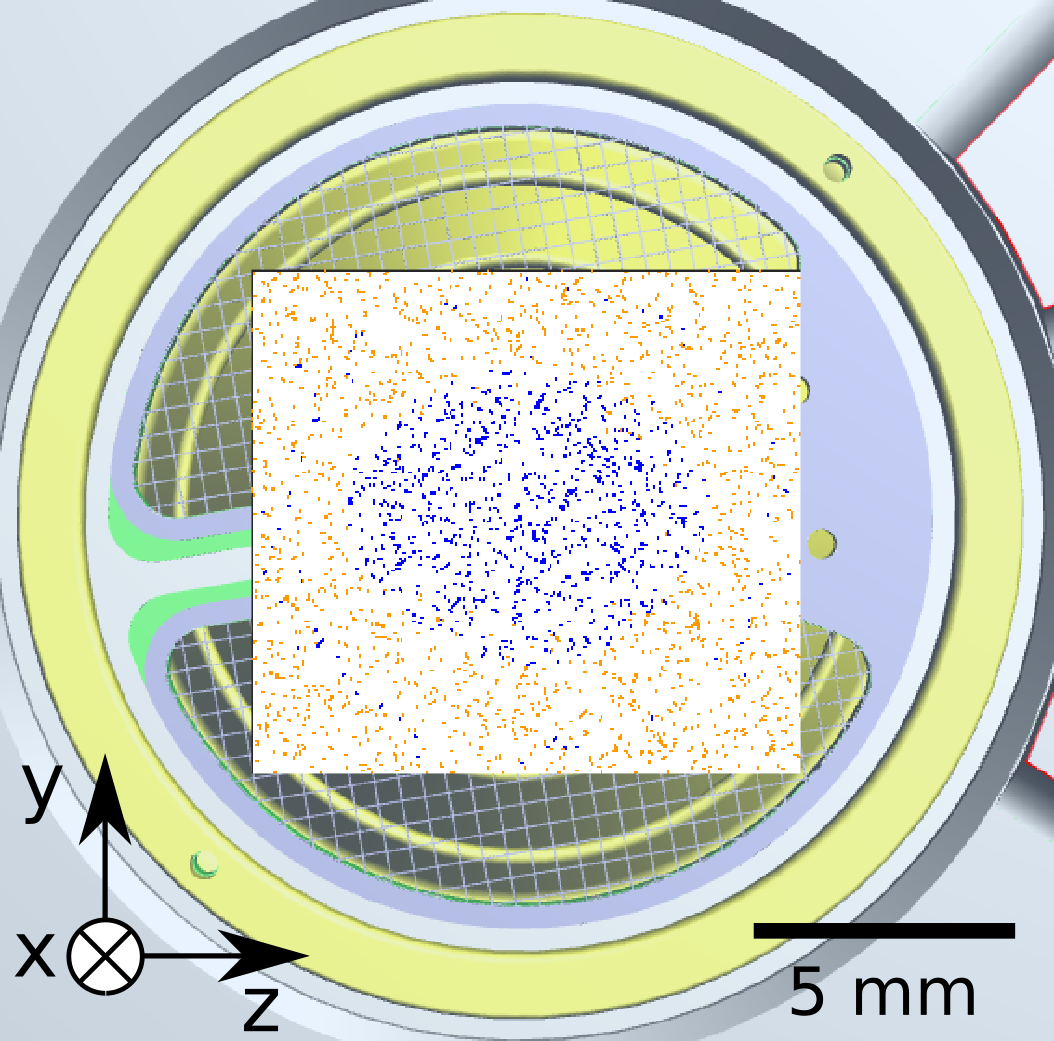
\includegraphics[width=.8\textwidth]{Experiments/PFMEntrance_Top_thSim.png}
			\caption{Top view, thermal mode.}
			\label{fig:PFMentrSideTopSimThTop}
		\end{subfigure}
		\begin{subfigure}[b]{.5\textwidth}
			\centering
			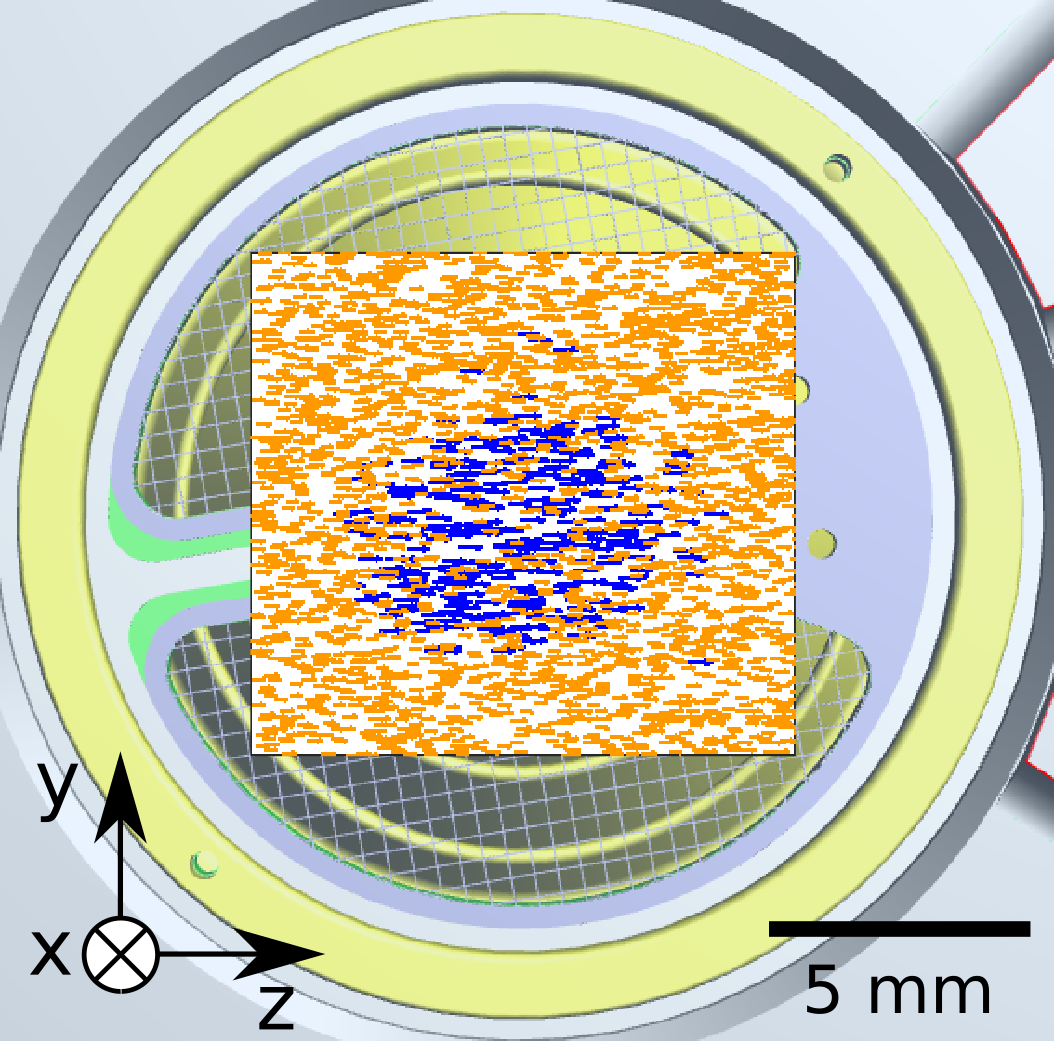
\includegraphics[width=.8\textwidth]{Experiments/PFMEntrance_Top_nSim.png}
			\caption{Top view, neutral mode.}
		\end{subfigure}
		\caption{Simulated ions marked as small arrows starting at different positions in the ionisation region. The simulated ions in n-Mode have a velocity of 4~km/s whereas the simulated ions in th-Mode have thermal velocity. The blue ions reach the detector whereas the orange ions hit the structure during their flight to the detector.}
		\label{fig:PFMentrSideTopSimthnMode}
	\end{figure}
	\begin{figure}[h] % Sim ions reach the detector i-Mode.
		\begin{subfigure}[t]{.5\textwidth}
			\centering
			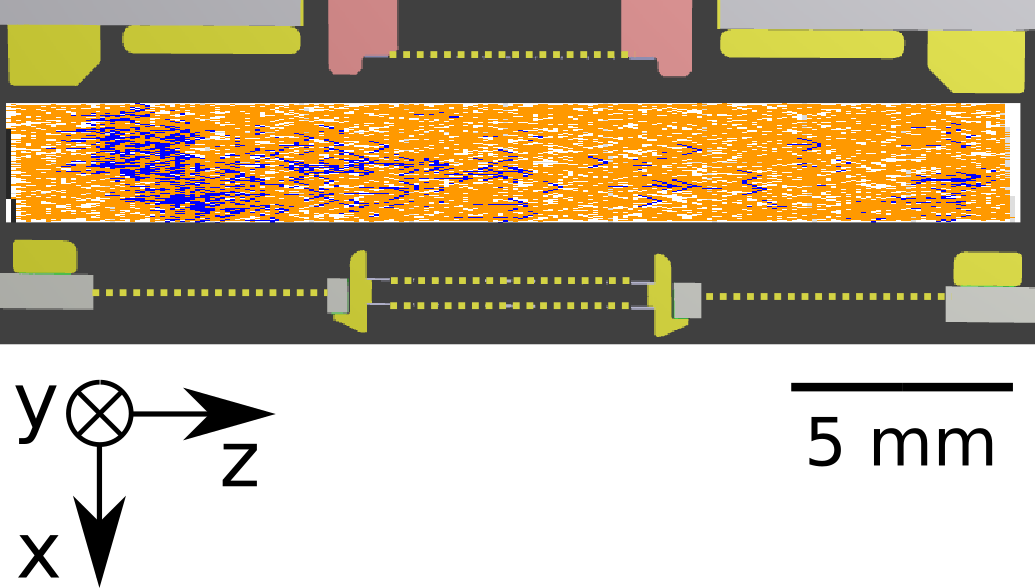
\includegraphics[width=.8\textwidth]{Experiments/PFMEntrance_Side_iSim.png}
			\caption{Side view, ion mode.}
		\end{subfigure}
		\begin{subfigure}[t]{.5\textwidth}
			\centering
			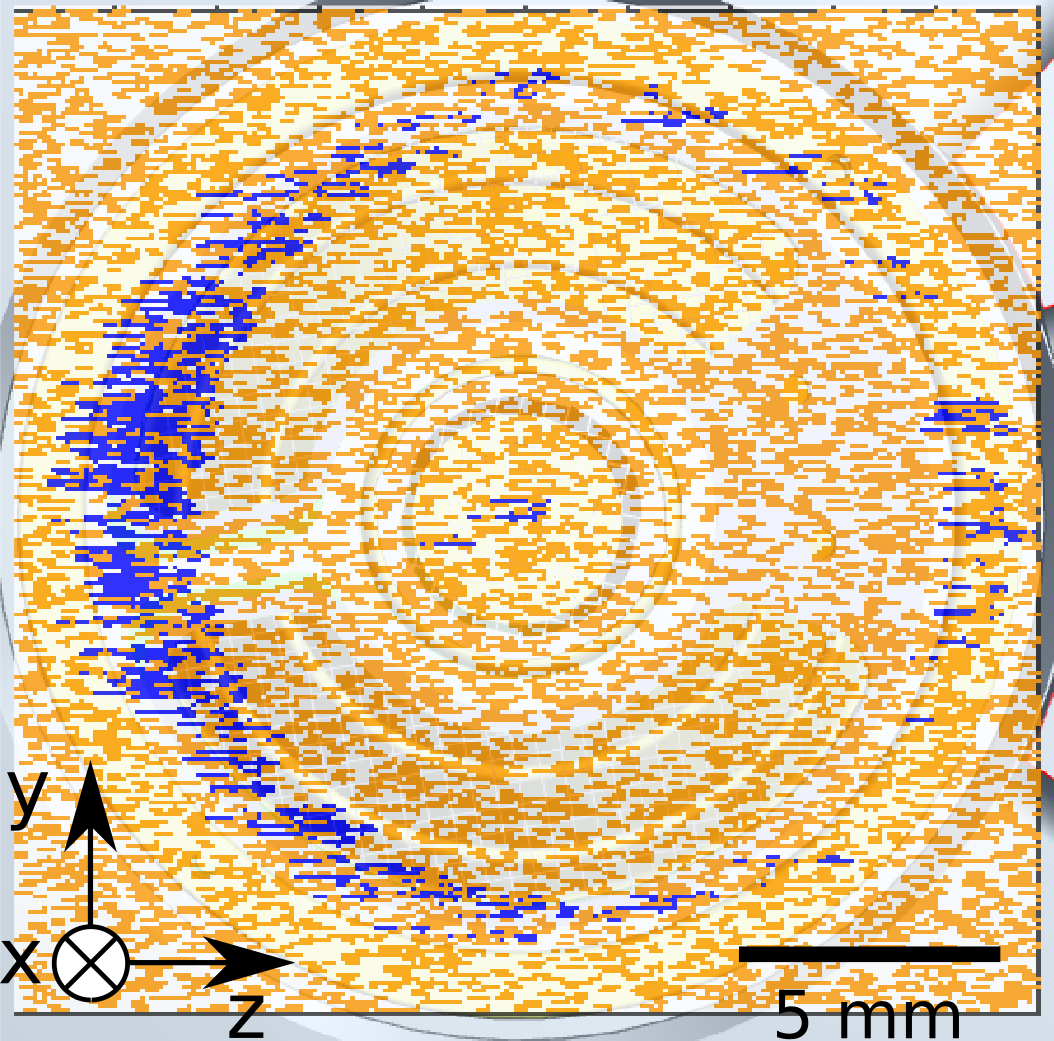
\includegraphics[width=.8\textwidth]{Experiments/PFMEntrance_Top_iSim.png}
			\caption{Top view, ion mode.}
		\end{subfigure}
		\caption{Simulated ions marked as small arrows starting at different positions in the entrance slit with a velocity of 4~km/s. The blue ions reach the detector whereas the orange ions hit the structure during their flight to the detector.}
		\label{fig:PFMentrSideTopSimiMode}
	\end{figure}
	\begin{figure}[h] % SIMION Model of i-Mode ion flight path.
		\centering
		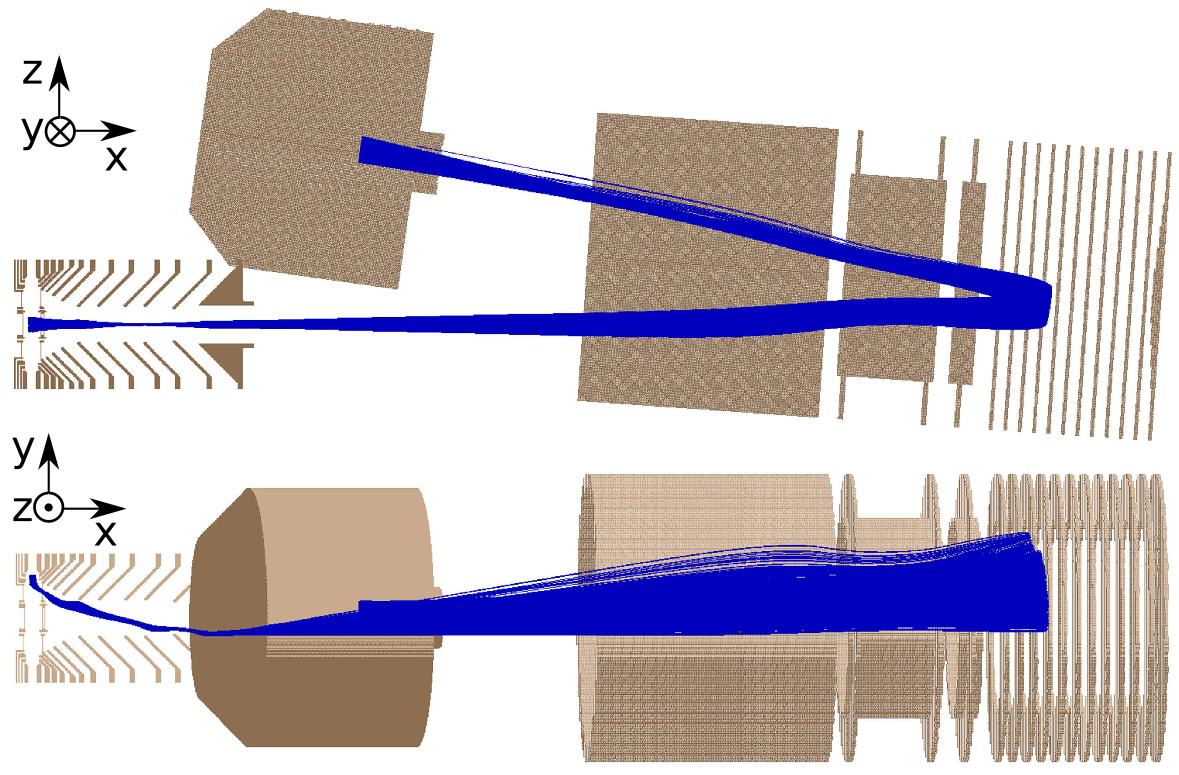
\includegraphics[width=.8\textwidth]{Experiments/Ionflys_imode.png}
		\caption{SIMION ion-optical model of the NIM prototype with ion trajectories in optimised i-Mode, arriving from the -y direction \cite{Diss_Meyer}.}
		\label{fig:iModeIonFlyStefan}
	\end{figure}
	\begin{figure}[h!] % Electron beam
		\centering
		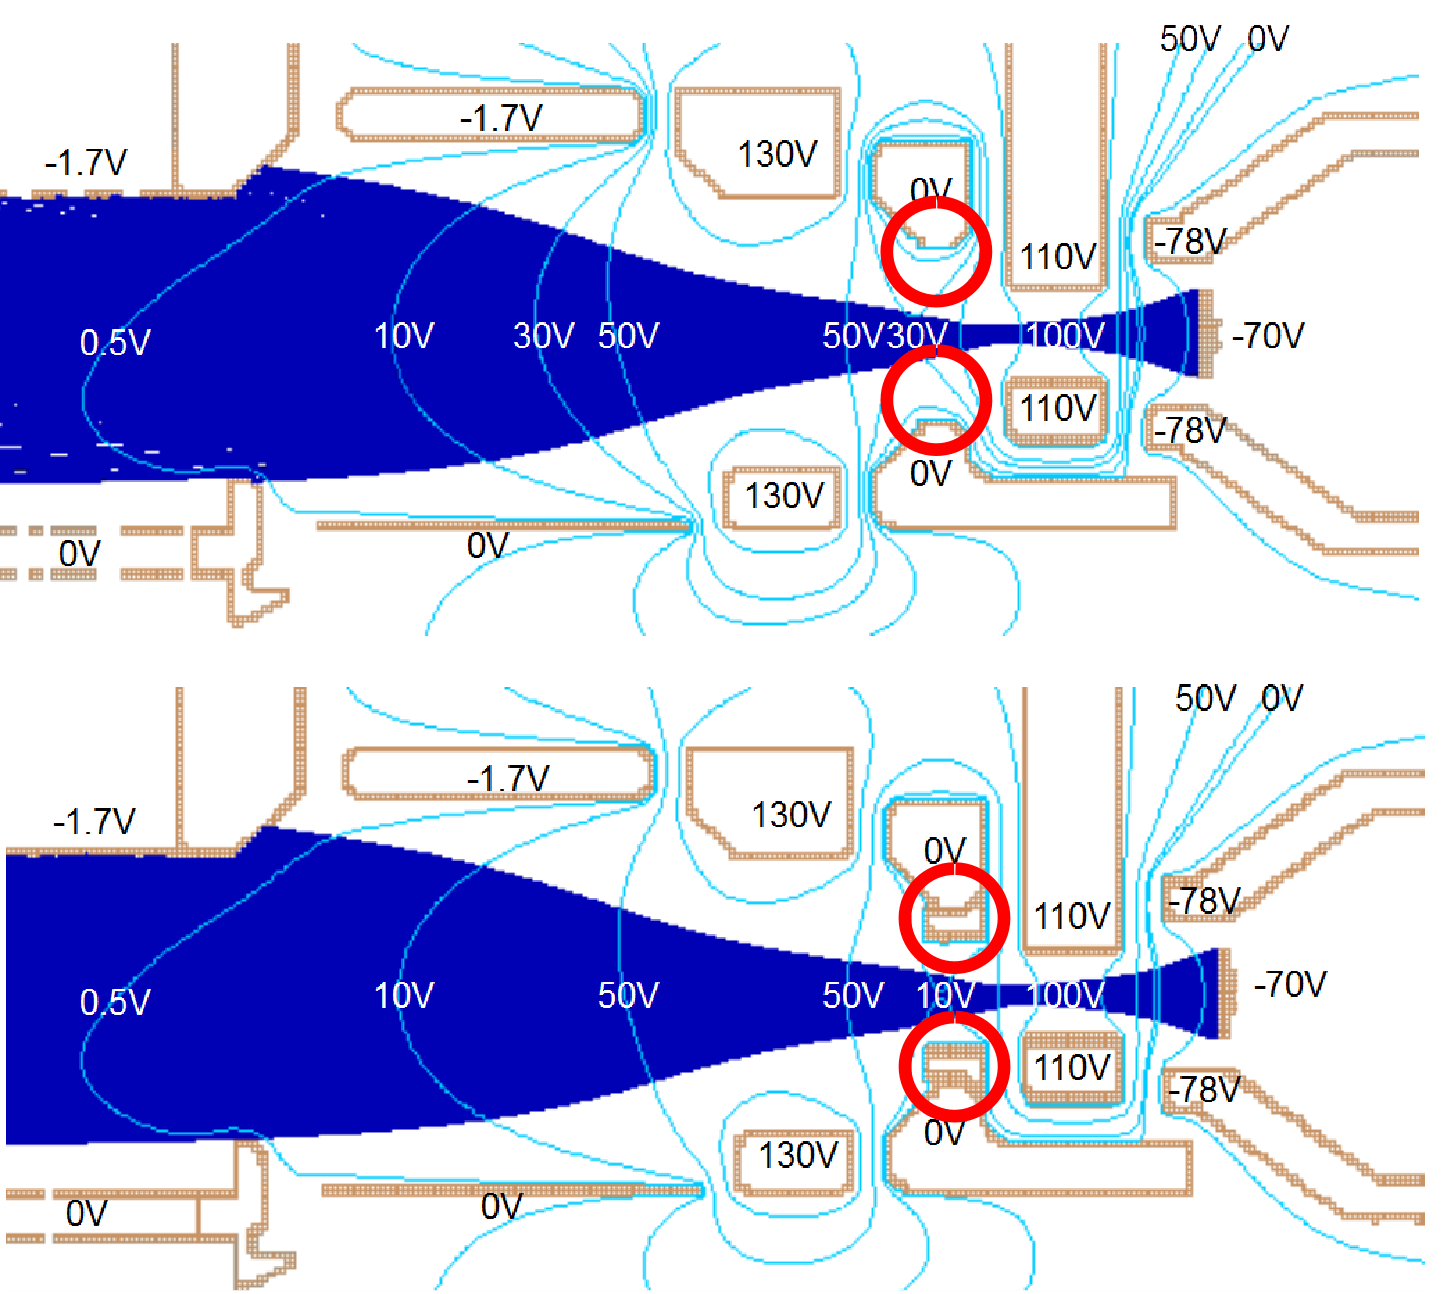
\includegraphics[width=.7\textwidth]{Experiments/IS_adaption.png}
		\caption{Top: New entrance with enlarged hole for the electron beam. Bottom: Old entrance with additional ring to reduce the diameter of hole.}
		\label{fig:IsAdapt}
	\end{figure}
	\begin{figure}[h]
		\centering
		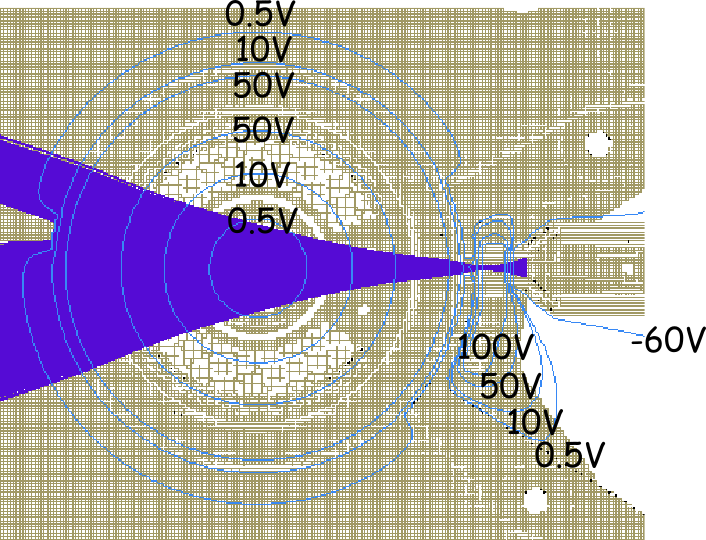
\includegraphics[width=.5\textwidth]{Experiments/IS_adaption_TopView.png}
		\caption{Top view onto the ionisation region of NIM with simulated electron beam trajectories (dark blue) and potential lines (light blue).}
		\label{fig:IsAdaptTop}
	\end{figure}
	can enter the ionisation region from every direction in the yz-plane except from where the filaments and the supporting structure are, resulting in a field-of-view of 300°. For the laboratory measurements, the gas inflow direction is from the bottom in the +y-direction as it is also shown in Fig.~\ref{exp:PFMIntCharEnt}. For the simulations, a gas inflow direction parallel to the electron beam was chosen as it is marked in Fig.~\ref{fig:PFMentrSideTopSchemas}, bottom panel. The generated ions of the th-Mode and n-Mode were generated in a cuboid volume with a height of 2~mm and a square base area of 8x8~mm. For the simulations of the i-Mode, the base area was 20x20~mm because the ions are pulled with the outer extraction grid into the spectrometer.\\
	Fig.~\ref{fig:PFMentrSideTopSimthnMode}~a) and c) show the simulated data for thermal mode where the incoming particles have thermal velocity. Fig.~\ref{fig:PFMentrSideTopSimthnMode}~b) and d) show the simulated data for the neutral mode and Fig.~\ref{fig:PFMentrSideTopSimiMode} shows the simulated data for ion mode where the incoming neutrals and ions respectively have a velocity of 4~km/s. The particles are displayed as velocity vectors. The ions marked in blue are the ones reaching the detector and the orange ones hit the structure somewhen during their flight to the detector. The simulated particles have unit masses from 1 up to 1000~m/z.	Fig.~\ref{fig:PFMentrSideTopSimthnMode} shows that only ions reach the detector that are generated directly above the inner extraction grid IS~5, which is also the one extracting the ions in thermal and neutral mode. In thermal mode, also some ions generated in the volume above the outer grid IS~6 reach the detector. They are visible as a small blue ring close to the structure separating the inner and the outer grid in Fig.~\ref{fig:PFMentrSideTopSimThTop})~c). In thermal mode the neutral particle flow comes through the pink structure and is directed over the inner pull grid. Therefore, only a small amount of gas reaches the outer grid. In neutral mode, only ions generated over the inner grid reach the detector due to their velocity perpendicular to the x-axis of the instrument. In ion mode, the ion optics are optimised for ions penetrating the ionisation region from the side as it is shown in Fig.~\ref{fig:iModeIonFlyStefan}. Due to their charge, ions react to the electric field as soon as they are close to the ion-optical lenses of the ionisation region. Their main starting position is therefore at the edge of the ionisation region and not in the centre as it is for the neutral particles. The ionisation of the neutral particles is optimised above the central extraction grid and therefore, most of the ions are generated above the inner extraction grid IS~5. When measuring with the ion mode, the ion-optical system is optimised for ions starting close the focusing lenses in the ionisation region as it is shown in the simulations in Fig.~\ref{fig:iModeIonFlyStefan} and Fig.~\ref{fig:PFMentrSideTopSimiMode}. The inner extraction grid is close to 0~V to additionally deflect the ions.\\
	Fig.~\ref{fig:IsAdapt} and Fig.~\ref{fig:IsAdaptTop} show the flight path of the electrons, which are used to ionise the neutral gas. During vibration tests of the ion-optical system, a weakness in the structure of the ion source was identified. This lead to a small redesign where the opening for the electron beam in the entrance electrode IS~3 had to be enlarged (Fig.~\ref{fig:IsAdapt}). Simulations were done to see how big the impact of that design adaption was. Fig.~\ref{fig:IsAdapt} bottom panel shows the old design with an additional ring to reduce the diameter of that hole and the top panel shows the new design without the ring in the entrance electrode. Dark blue lines are the flight paths of the electrons and light blue lines show the electric potential lines. The adaption of IS~3 had not impact on the flight path of the electrons. As previously discussed, the aim is to ionise the neutral particles in the cylinder volume above the inner pull grid efficiently because only ions generated in this volume will reach the detector. Therefore, the electron beam should cover the whole cylinder volume. Fig.~\ref{fig:IsAdaptTop} shows the top view from the ionisation region. The porous ring structure is the outer extraction grid IS~6. The inner grid is not visible because it is covered by the electron beam. In this model, only one filament is displayed. Between the two potentials lines which mark the 50~V ring is electrode IS~4 which is on 130~V. Fig.~\ref{fig:IsAdapt}~top and Fig.~\ref{fig:IsAdaptTop} show, that with the applied voltages the electron beam covers the whole volume over the inner extraction grid.
	
	% Intensitätssimulation Countberechnung filament:
	% Man generiert 2000 e- auf dem Filament und zeichnet immer nach 1E-5 microsec auf, an welcher Position sich die Teilchen gerade befinden. Die Fkt. 'Plot_optVoltAndPos.m' zählt alle Positionen zusammen, welche sich in dem Zylindervolumen befinden. Die Grundfläche des Zylinders ist das Eintritts-Grid von der antechamber und die Höhe ist die Höhe der Entrance. Im th-Mode befinden sich nur in diesem Volumen neutrale Teilchen.
	
%----------------------------------------------------------------------------------------
	\subsection{Shutter Performance Test}\label{chap:expShutter}
	When measuring with the neutral gas channel, the aim is that the particles are measured directly without any interaction with the structure of the instrument. Therefore, a shutter between the antechamber and the ionisation region was required to close the particle entrance from the antechamber. In this section the performance of the shutter was tested. According to the model stated in Chap.~\ref{subsubsec:motorflow} the closed shutter should attenuate the signal in the ionisation region generated by particles from the antechamber by a factor 600.\\
	These tests were performed with the NIM PFM. The PFM was operated with laboratory electronics. The tests were performed at the CASYMIR test facility. The used particle beam consisted of hydrogen and xenon with a velocity of 2~km/s. Three different measurements were performed: One with the beam directed onto the antechamber with the shutter open, one with the shutter closed and a background measurement, where the particle beam was pointed onto the outer structure of NIM to estimate how much of the signal arises from the test gas scattering into the ionisation region when the beam is directed in an arbitrary direction. This background was subtracted from both signals before they were divided through each other to determine the attenuation factor $G_{close}$ of the shutter.\\
	The resulting attenuation factor of the shutter is 12 instead of the required 600 with a proper fabricated shutter. The biggest impact has the actual thickness of the gap between the shutter and the antechamber when the shutter is closed. The reduction becomes significantly lower when the gap is bigger than actually designed. This is shown in Fig.~\ref{fig:ShutGapSizeSigDamp} in Chap.~\ref{subsubsec:motorflow}. With a gap size of about 0.1~mm instead of 0.01~mm the attenuation factor is only about a factor 25. Other reasons are that the portion of the beam that scatters on the antechamber outer walls gets thermalised in the vacuum chamber and adds to the signal intensity in the neutral channel, which is estimated to contribute equally to the measured signal. In the outer space, the gas scatters on the antechamber but does not reach the ionisation region because it will flow around the instrument.
	
%--------------------------------------------------------------------------------------------
	\subsection{Pulser} \label{chap:ExpPulser}
	The high-voltage pulse generator (pulser) is used to accelerate the generated ions in the ionisation region to a certain energy. During the time when no high voltage pulse is applied, the potential has to be stable at the bias voltage to allow ion storage as previously discussed in Chapter~\ref{chap:TheoIonStor}.\\
	Fig.~\ref{fig:PulserTheoCurve} shows a schema of a realistic high voltage pulse and Table~\ref{tab:FlightPulserPerf} shows the characteristics of the flight pulser compared to the requirements. The fall time is the time to build up the negative high voltage on the extraction grid. This time has to be very short to give all ions the same amount of energy. When the fall time is long, low mass ions receive less energy resulting in a lower mass resolution for these species. A fall time of 1~ns leads to a 0.1~\% lower mass resolution of hydrogen compared to an ion with mass 200~u. A fall time of 5~ns results in a reduction by 10~\% (see Chap.~\ref{chap:massRes}). The fall time of the flight pulser is a bit longer than according to the specifications.\\
	\begin{figure}[H]
		\centering
		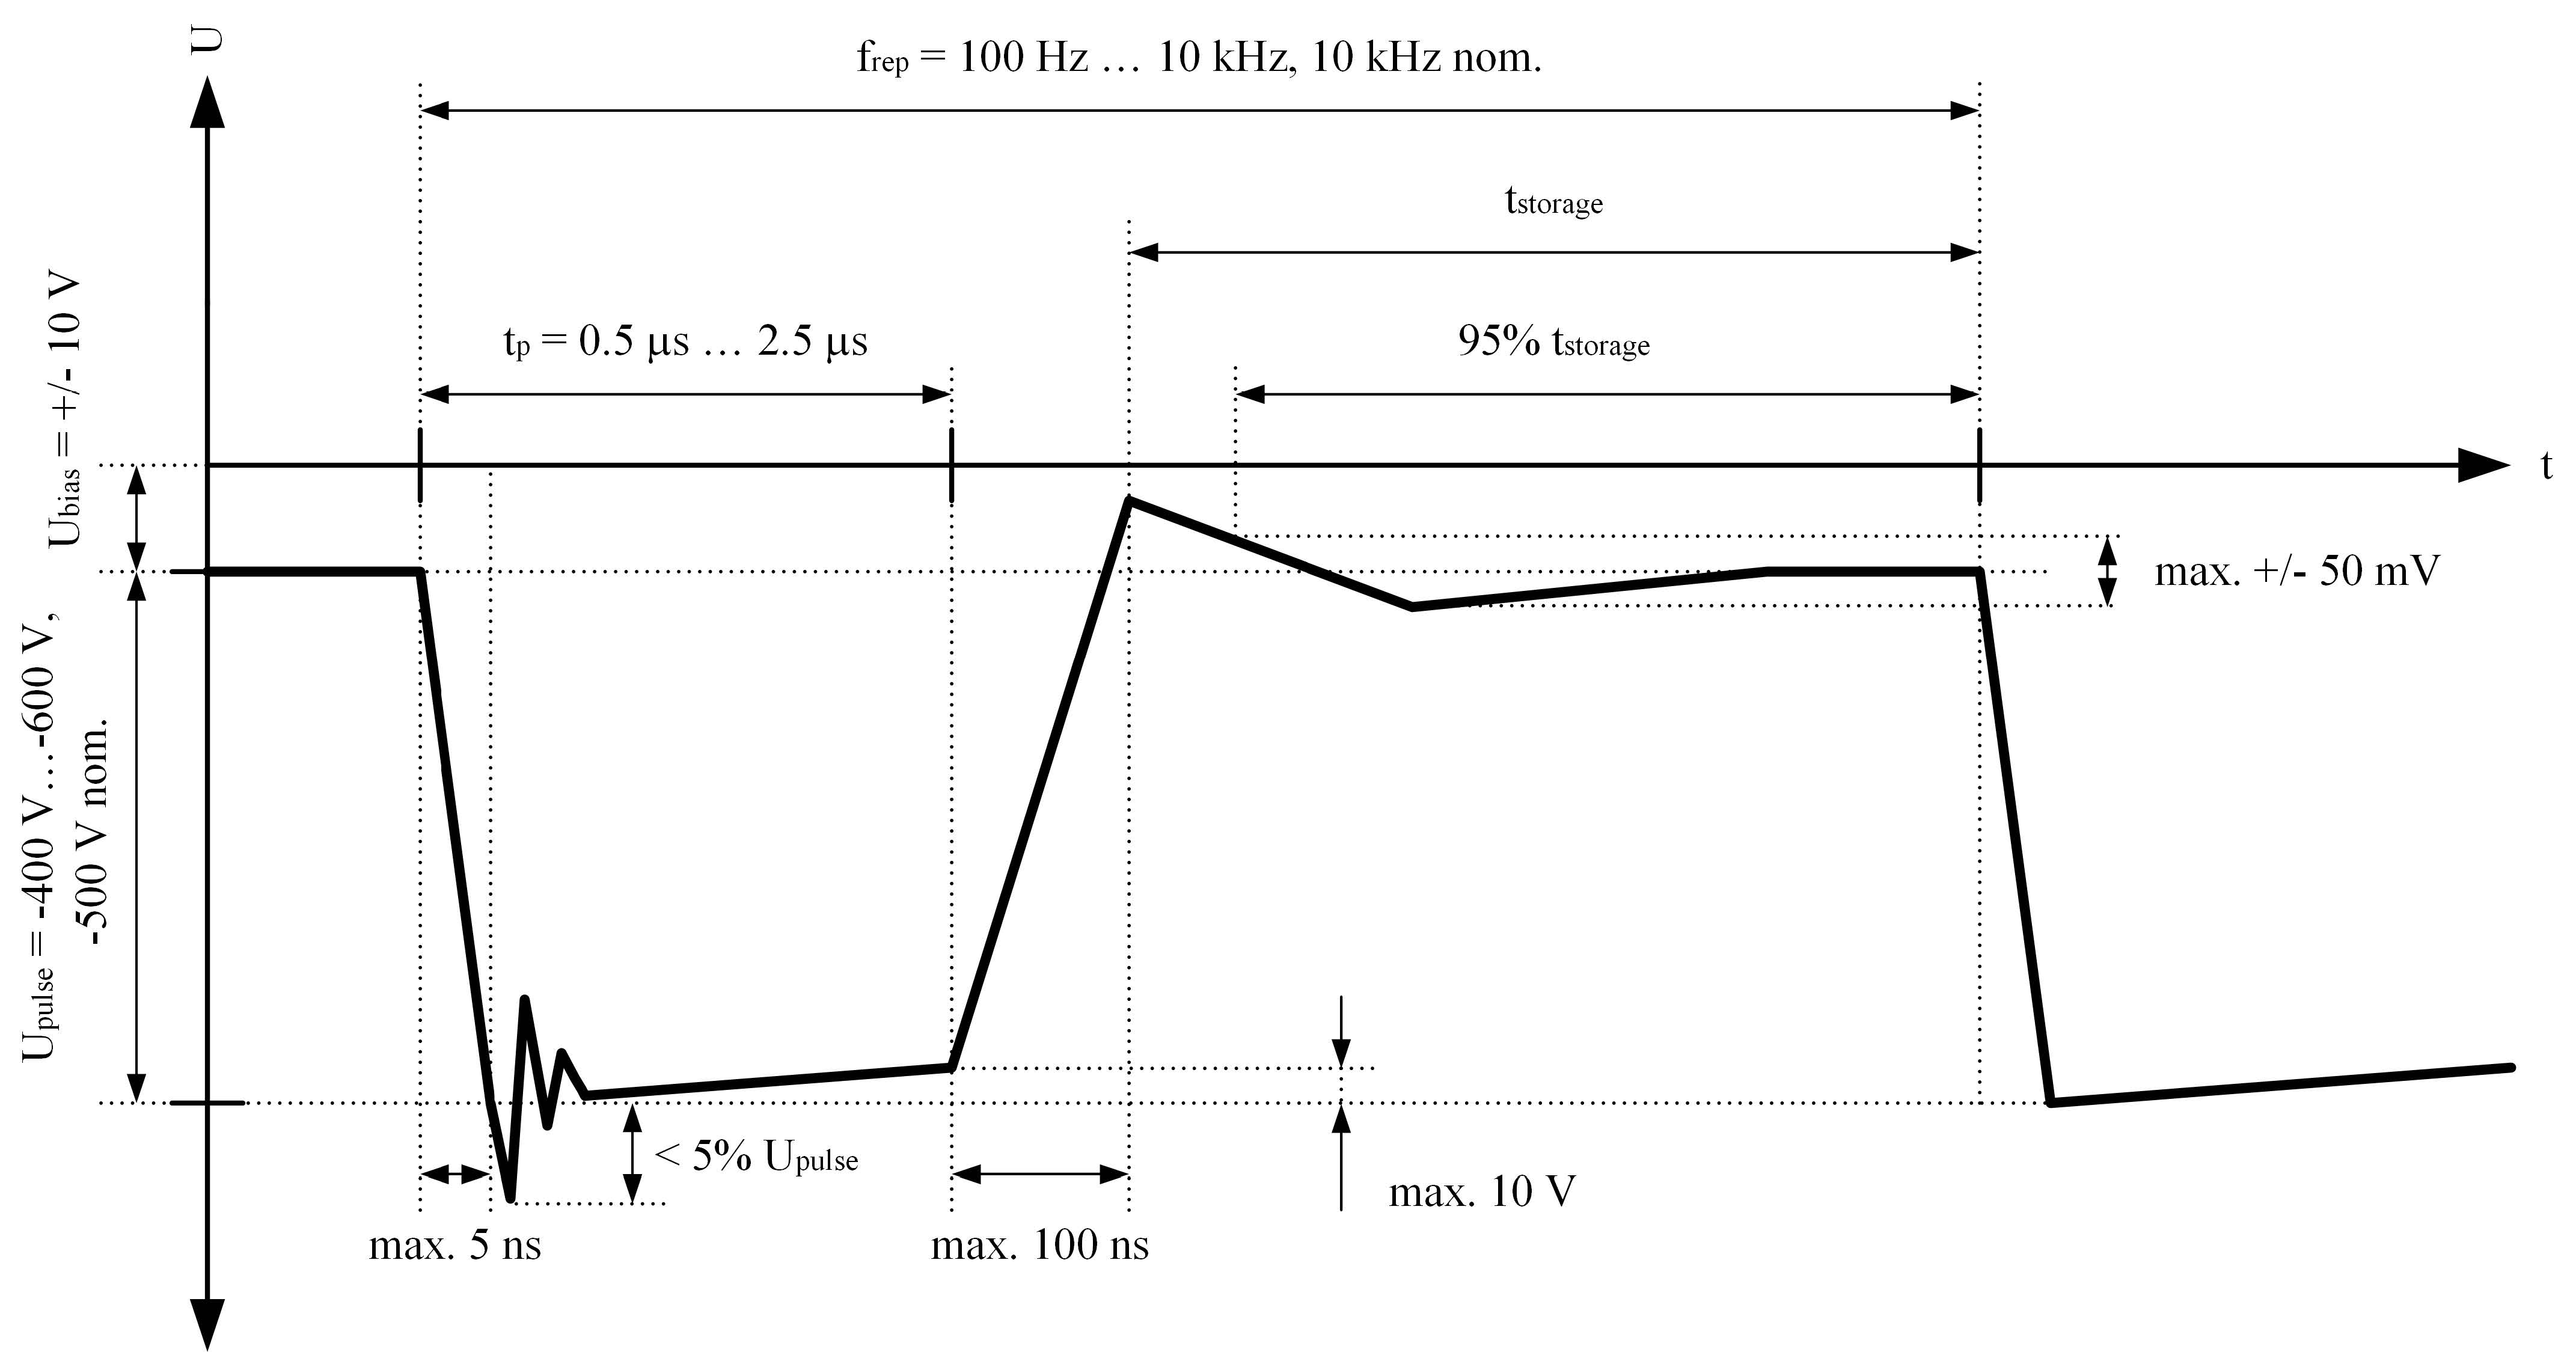
\includegraphics[width=\textwidth]{Bilder/Pulser_theretical_shape.jpg}
		\caption{Specifications for the pulse shape generated by a realistic pulser \cite{Diss_Meyer}.}
		\label{fig:PulserTheoCurve}
	\end{figure}
	\pagebreak
	\begin{table}[H]
		\begin{center}
			\begin{tabular}{|m{2.2cm}|>{\centering}m{2cm}|>{\centering}m{2cm}|>{\centering}m{2.8cm}|>{\centering}m{1.7cm}|m{1.8cm}<{\centering}|}
				\hline
				& Ringing of HV Pulse & Pulse drop at full HV & Baseline Ripple & Fall Time & Rise Time \\ \hline
				Requirement		& $<$ 5\%  & $<$ 10~V & $\pm$50~mV & $<$ 5~ns & $<$ 100~ns\\
				Flight Pulser	& 2.5\% & 1.9~V & 300~mV & 5.76~ns & 19.7~ns\\
				\hline
			\end{tabular}
		\end{center}
		\caption{Characteristics of the flight pulser compared with the requirements.}
		\label{tab:FlightPulserPerf}
	\end{table}
	When applying a high voltage, the pulse overshoots its set value and drops slightly. The overshoot and the voltage drop result in a variation of the ion energy for the different species. The ringing of the high voltage, and the pulse drop of the flight pulser are within the specifications. The pulse duration has to be longer than 2~\si{\micro\second} because that is the minimum time ions with masses of 1000~u need to leave the ionisation region. With some margin, the specifications were set to 5~\si{\micro\second}. The rise time to bias voltage should be smaller than 100~ns to leave enough time for ion storage. This is well achieved with the flight pulser. The ripple of the bias voltage should be smaller than $\pm$50~mV to generate a stable electric field during the time when no high-voltage is applied on the extraction grid. A variation by $\pm$100~mV of the voltage of the electrode opposite of the pulser grid results in a visible variation of the signal intensity during manual optimisation with laboratory electronics. However, the baseline ripple of the flight pulser exceeds this value.


%--------------------------------------------------------------------------------------------
	\subsection{Detector Tests}\label{chapExp:Det}
	% To be added if there is time. Data from the detector before and after TVT.
	
	\begin{figure}[h] % Flat and folded detector. Make notes of the different parts.
		\centering
		\includegraphics[width=.7\textwidth]{Experiments/Detectors_fla_folded.png}
		\caption{NIM flight detectors ready for tests. Top: flat configuration. Bottom: folded configuration.}
		\label{fig:DetFlatFolded}
	\end{figure}
	\begin{figure}[h!] % Detector gain curves during conditioning of both FS detectors.
		\begin{subfigure}{.5\textwidth}
			\centering
			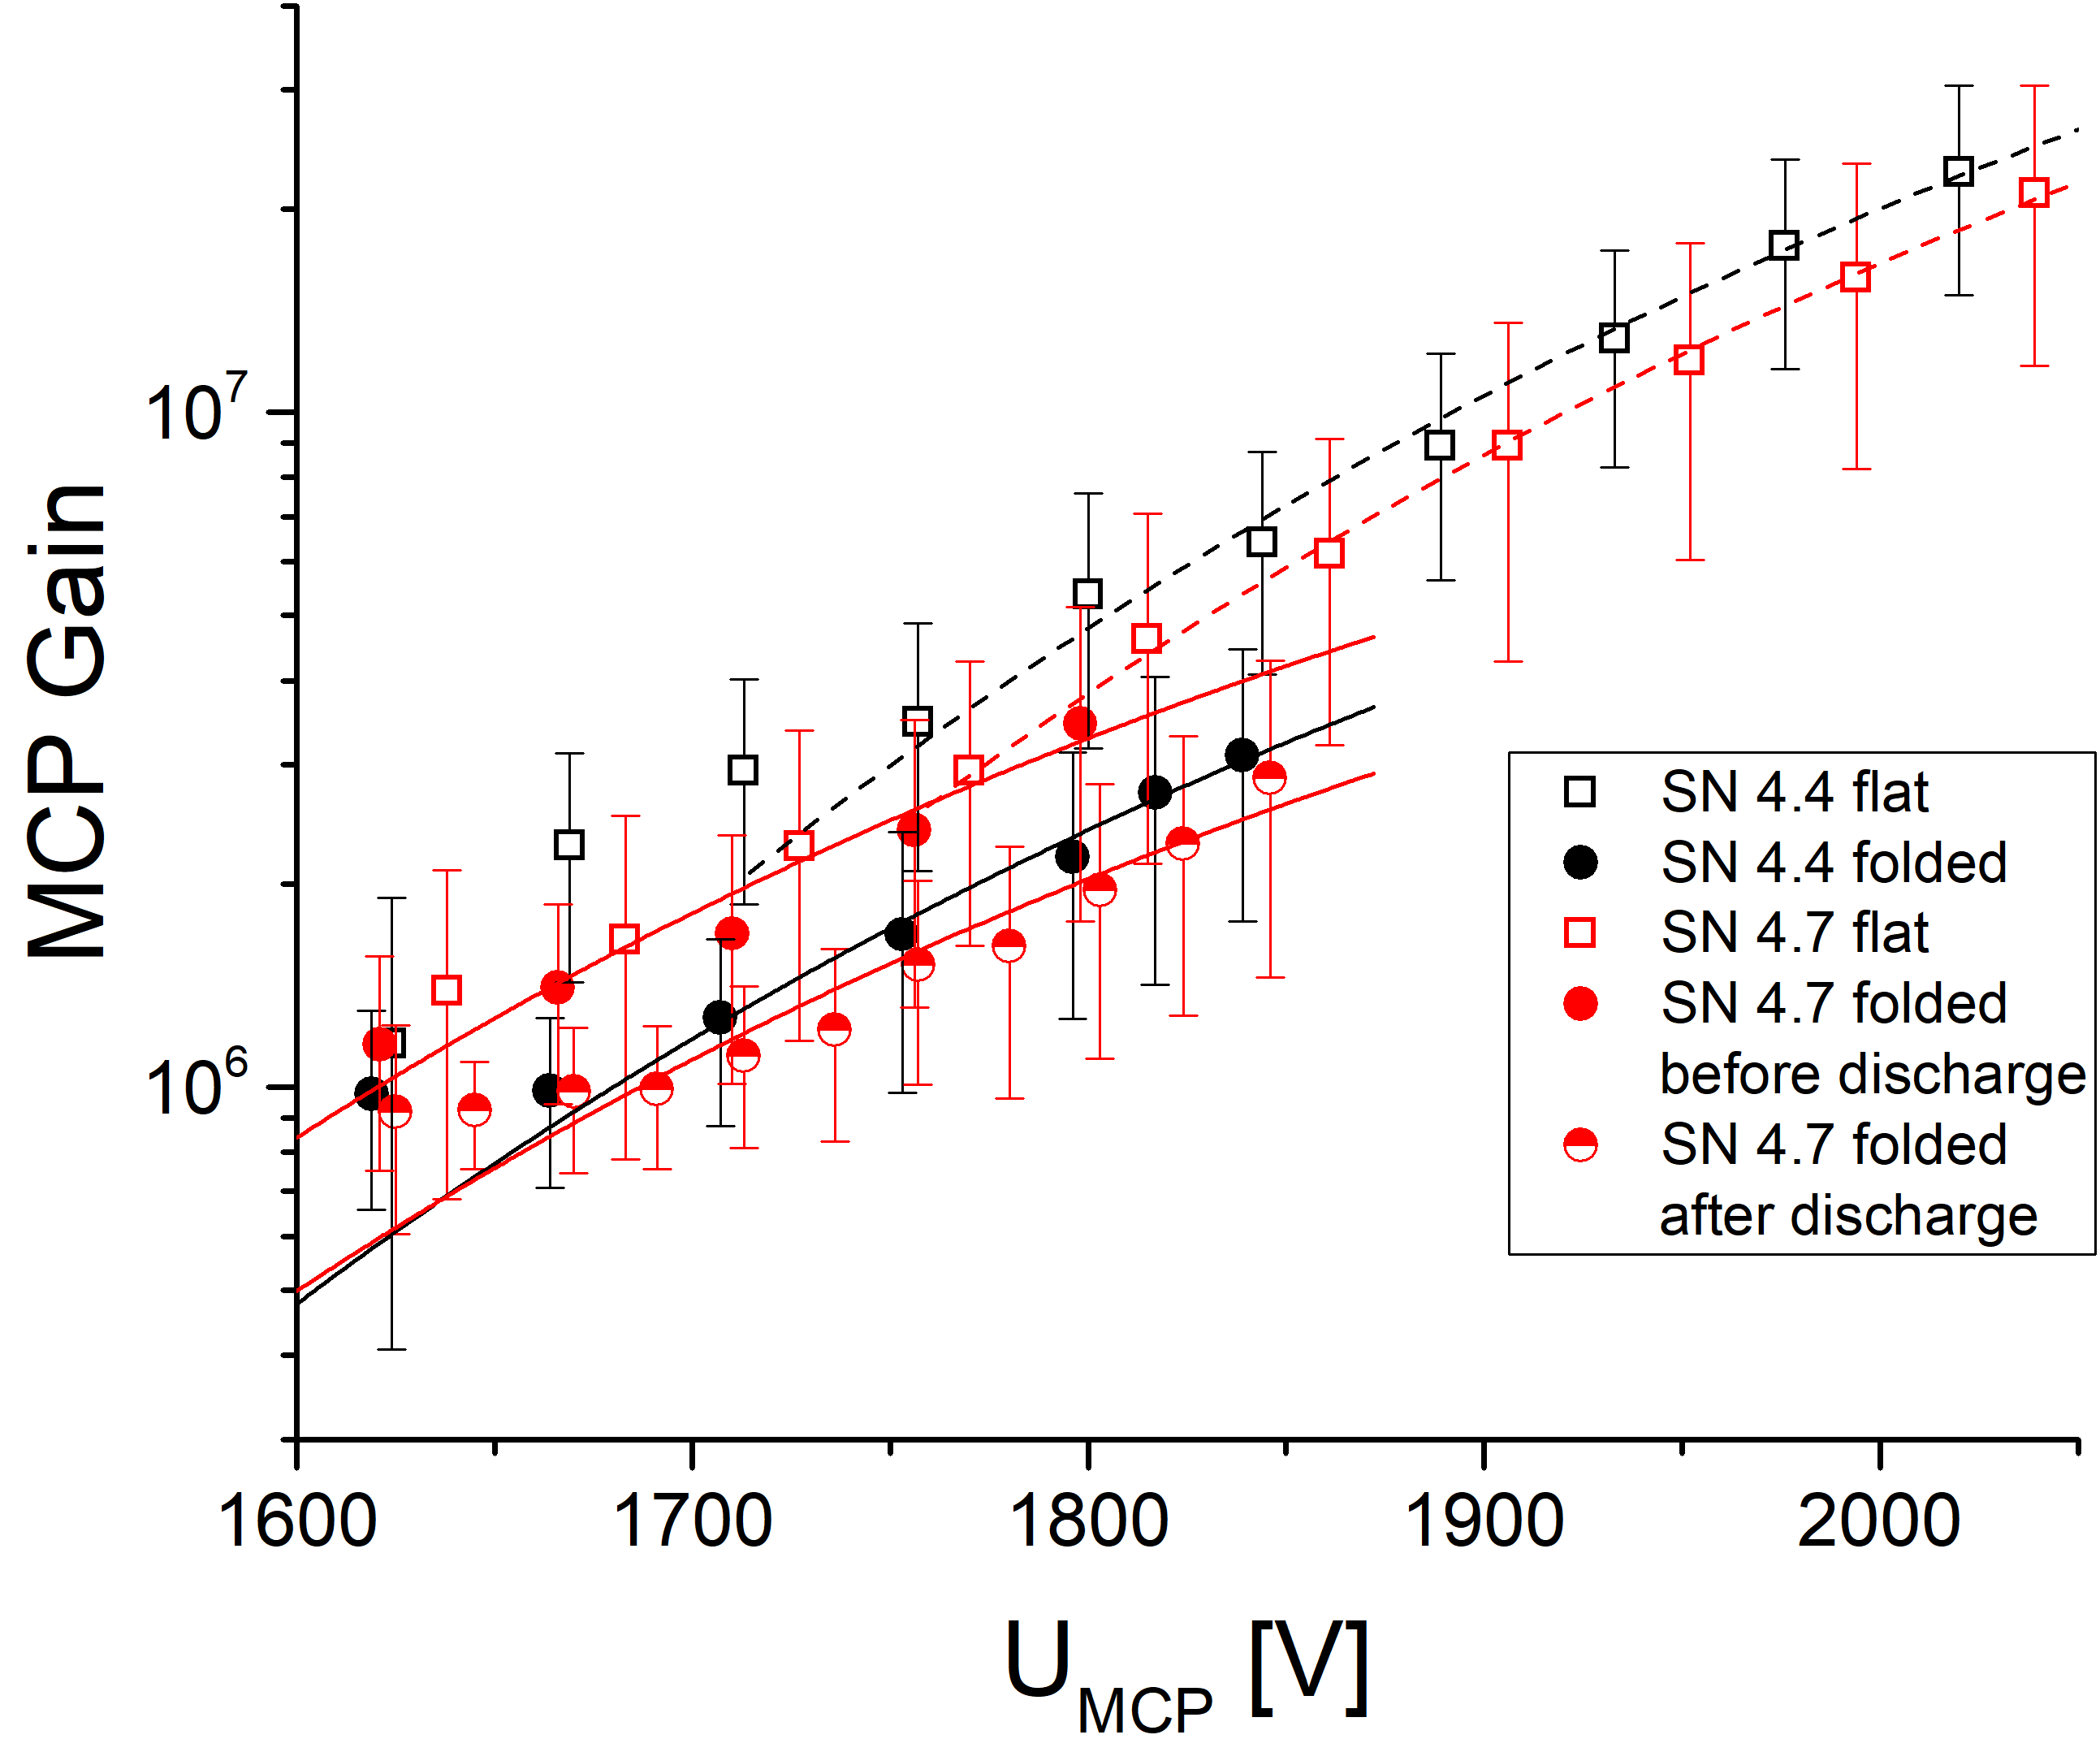
\includegraphics[width=0.9\textwidth]{Experiments/Gain_Curves_SN4p5_4p7.png}
		\end{subfigure}
		\begin{subfigure}{.5\textwidth}
			\centering
			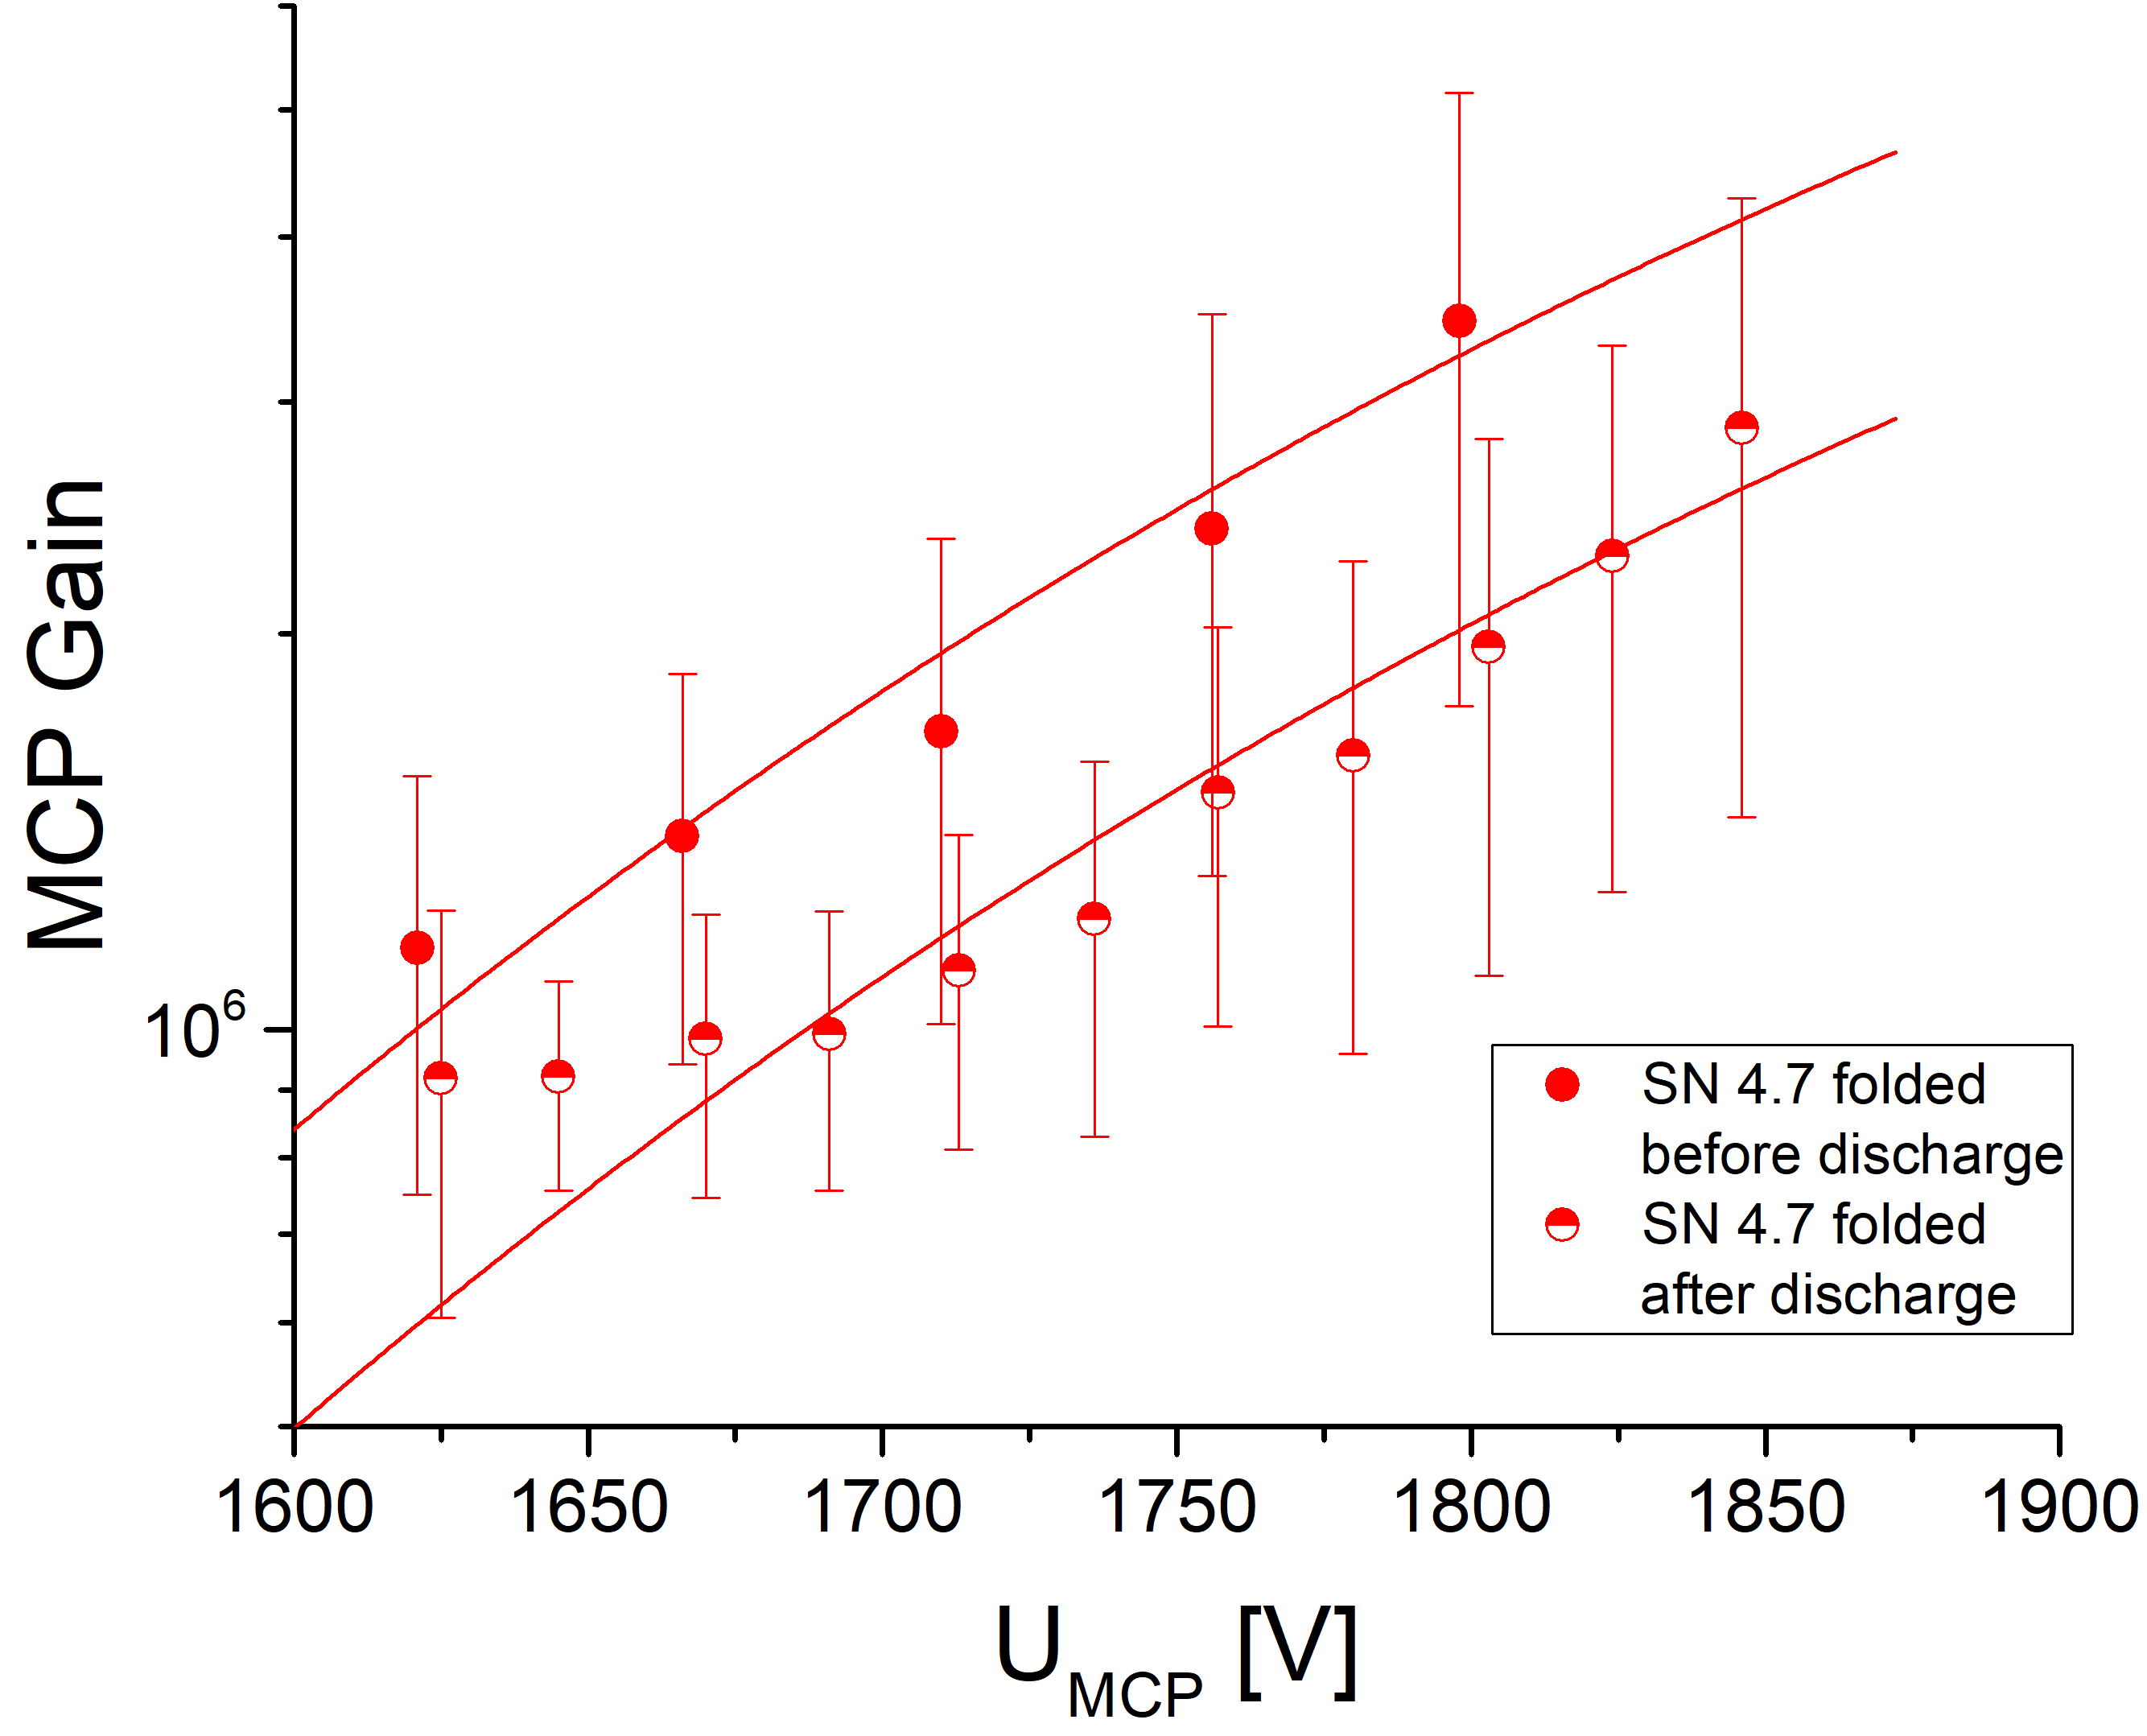
\includegraphics[width=0.9\textwidth]{Experiments/SN4p7_discharge.png}
		\end{subfigure}
		\caption{Left: Gain curves of two NIM FS detectors, in flat and in folded configuration (see Fig.~\ref{fig:DetFlatFolded}). The difference in gain is because for each measurement curve, a different set of MCPs was used. Right: Gain curves of a folded NIM FS detector. The lower gain curve was recorded after a discharge at an MCP voltage of 1.8~kV.}
		\label{fig:SN4p54p7Gain}
	\end{figure}
	This chapter describes the testing procedure of the flight detectors and shows the calibration results. The flight detectors consist of a flexible PCB (Printed Circuit Board) for the proximity electronics, accommodated within a PEEK housing for the MCPs (Chap.~\ref{sec:setup}). Due to Jupiter's harsh radiation environment, the NIM detector has to be shielded with a tungsten copper shielding of about 1.1~kg. To minimise the shielding mass, a flex PCB was used to fold the detector with its proximity electronics into the small PEEK structure to minimise the detector volume. The detectors are tested in flat configuration with test MCPs and in folded configuration with flight MCPs (Fig.~\ref{fig:DetFlatFolded}). The detectors were put in a vacuum chamber and baked out for 2~days. The conditioning was started one day after bake out when a residual gas pressure in the chamber lower than $5\cdot10^{-8}$~mbar was reached. Since the detector has lots of enclosed volumes, sufficient time for their evacuation has to be foreseen. The conditioning procedure is attached in the Appendix Chap.~\ref{sec:appendix}. Depending on the outgasing behaviour of the detector, the conditioning took 2.5 to 4.5~h. After the conditioning, the measurements of the detector gain were performed.\\
	Fig.~\ref{fig:SN4p54p7Gain}, left panel shows the gain curves of two FS detectors in flat and folded configuration (see Fig.~\ref{fig:DetFlatFolded}). The conditioning and the measurements in the folded configuration were done only up to lower voltages to minimise the usage of the potential flight MCPs. The gain of the MCPs depends on different factors. As described in Chapter~\ref{sec:DetParam} the MCP gain is a strong function of the voltage applied over the MCPs as it is shown in Fig.~\ref{fig:SN4p54p7Gain}. With usage given by the amount of the extracted charge from the MCPs, the MCPs degrade over time. This process depends on the residual gas pressure at which the MCPs are operated and the residual gas composition. The rapid decline in gain during the first few operation hours is a result of cleaning the channels mostly from water through operation (Fig.~\ref{fig:MCPrelGainTime}). When the MCPs were exposed to air, water and other substances deposit in the MCP channels. During operation, these deposits are sputtered from the channel surfaces, and thus the surface of the channels 
	\begin{figure}[H] % Theoretical gain curve as a function of time
		\centering
		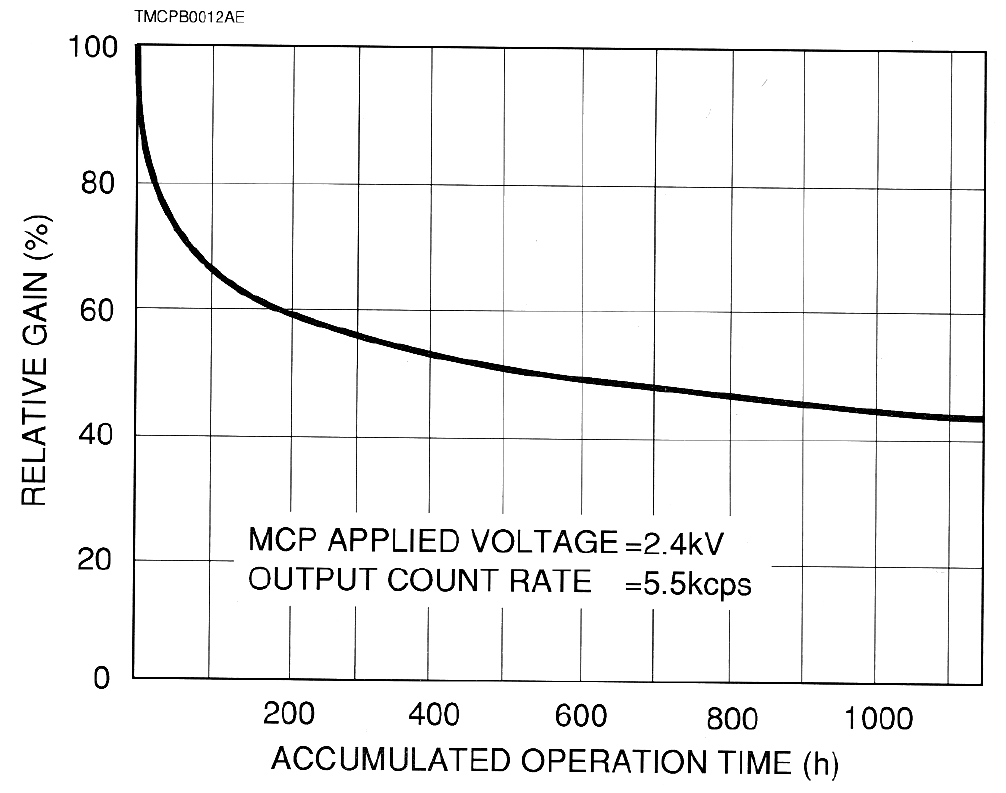
\includegraphics[width=.5\textwidth]{Experiments/MCP_relGain_timeevol.png}
		\caption{Relative gain of an MCP as a function of operation time \cite{LecNot_Wurz2017}.}
		\label{fig:MCPrelGainTime}.
	\end{figure}
	\begin{figure}[H]
		\centering
		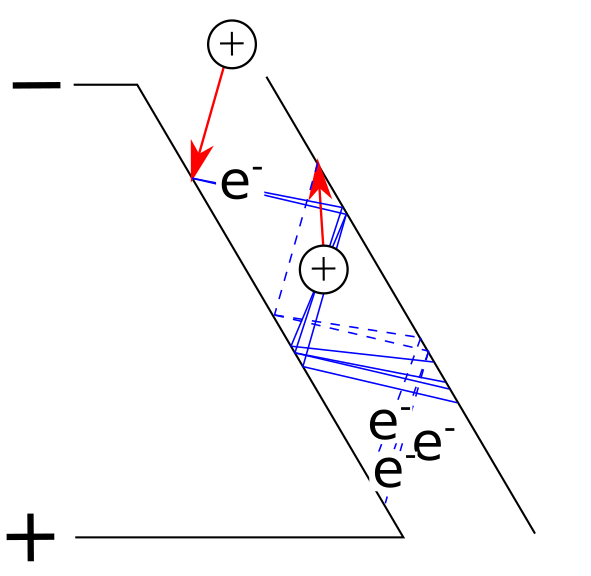
\includegraphics[width=.3\textwidth]{Experiments/DischargeMod.png}
		\caption{One single MCP channel when an ion triggers and electron avalanche. The ion in the channel centre is generated by the electrons when the gas pressure in the channel is too high.}
		\label{fig:expDischMod}
	\end{figure}
	 are cleaned. After a few hours of operation, the gain reaches a plateau. In flat configuration detector SN~4.7 has a lower gain than SN~4.4 because its conditioning took longer than the conditioning of detector SN~4.4. Therefore it was cleaned better. In the folded state, SN~4.4 was 3~days longer in vacuum than SN~4.7 and had therefore more time to outgas. Fig.~\ref{fig:SN4p54p7Gain} right shows a zoom on the two measurement series of SN~4.7 both recorded in folded configuration. During the first measurement series, a discharge happened when the MCP voltage was at 1.8~kV. To amplify a signal, a minimal voltage has to be applied over the MCPs. When they are barely used, this voltage is in the range of 1.6~kV. During ageing, the decrease in gain can be compensated by increasing the MCP voltage. When an ion induces an electron avalanche, the electrons are freed in the channel and their main moving direction is towards the channel output because of the electric field applied over the MCPs (Fig.~\ref{fig:expDischMod}). If the local pressure in the MCPs is too high, the electrons ionise the gas in the channels and generate positive ions. These ions are accelerated back towards the MCP front and eject other electrons 
	\begin{figure}[h!] % FS gain Curve
		\centering
		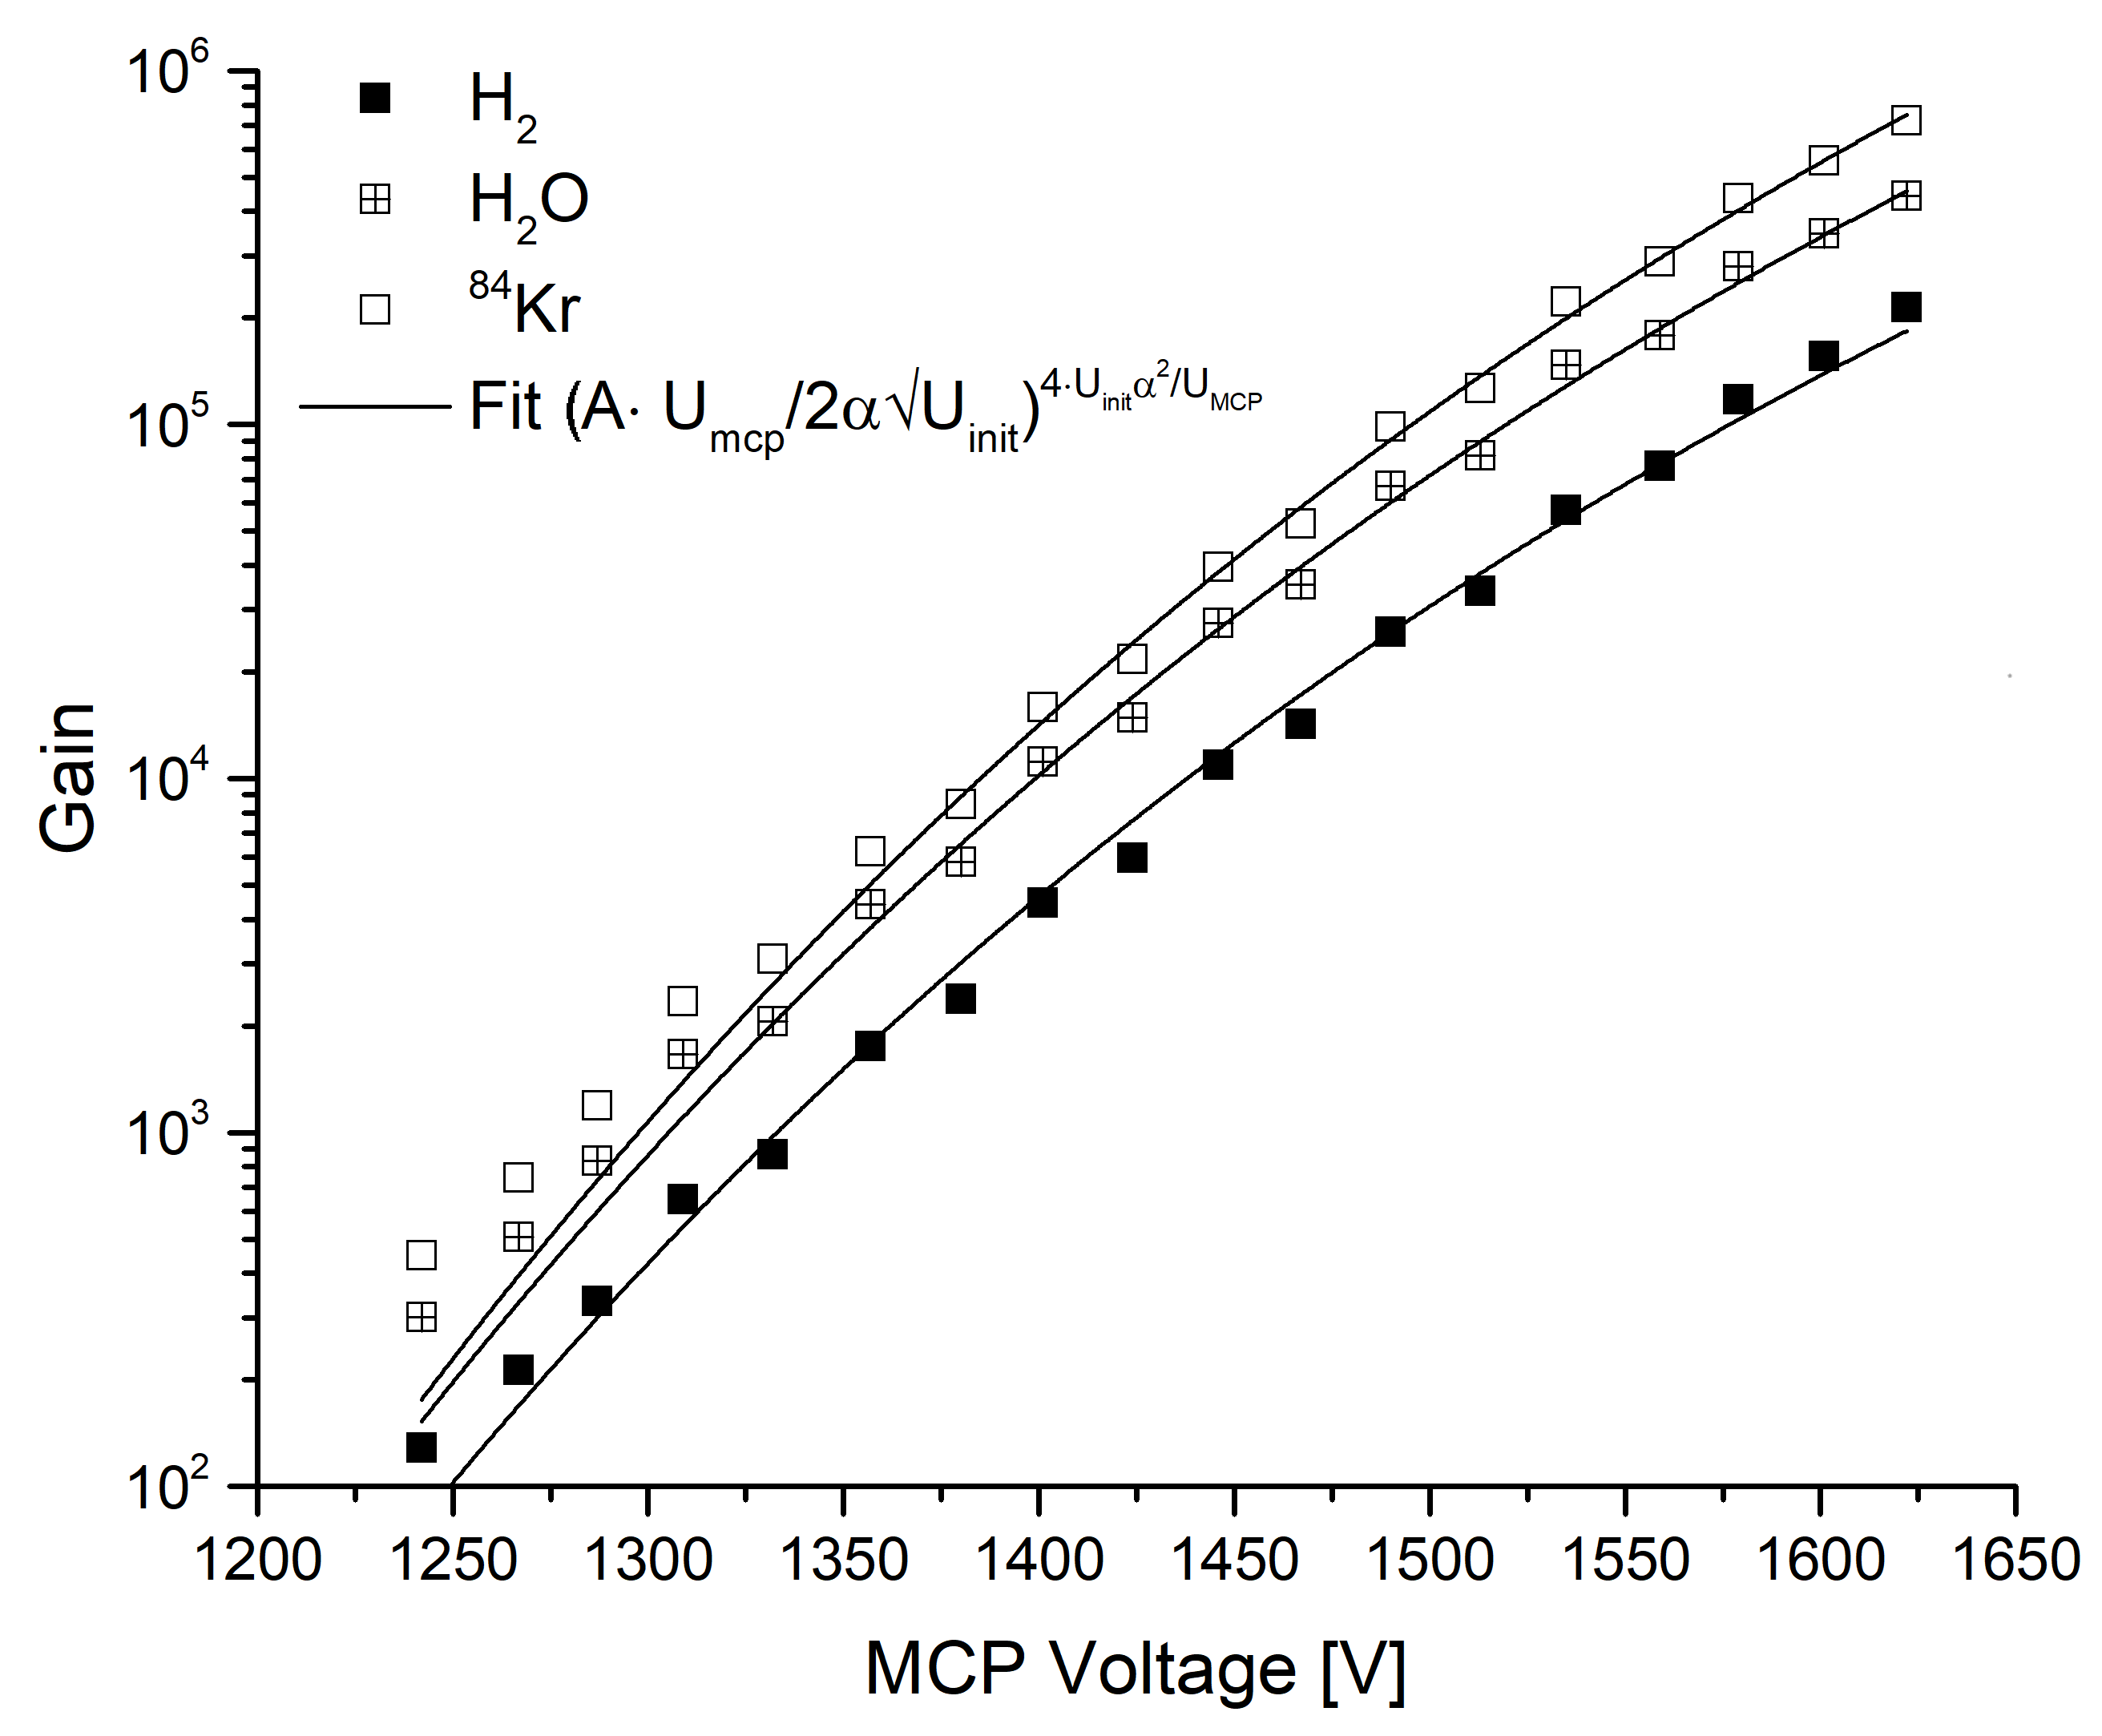
\includegraphics[width=.7\textwidth]{Experiments/GainDetFSLabEl.png}
		\caption{Gain curves of the detector SN~4.7 measured with the NIM FS ion-optical system.}
		\label{fig:MCPGainCurve4p7}
	\end{figure}
	\begin{figure}[h!] % Calibraton curve
		\centering
		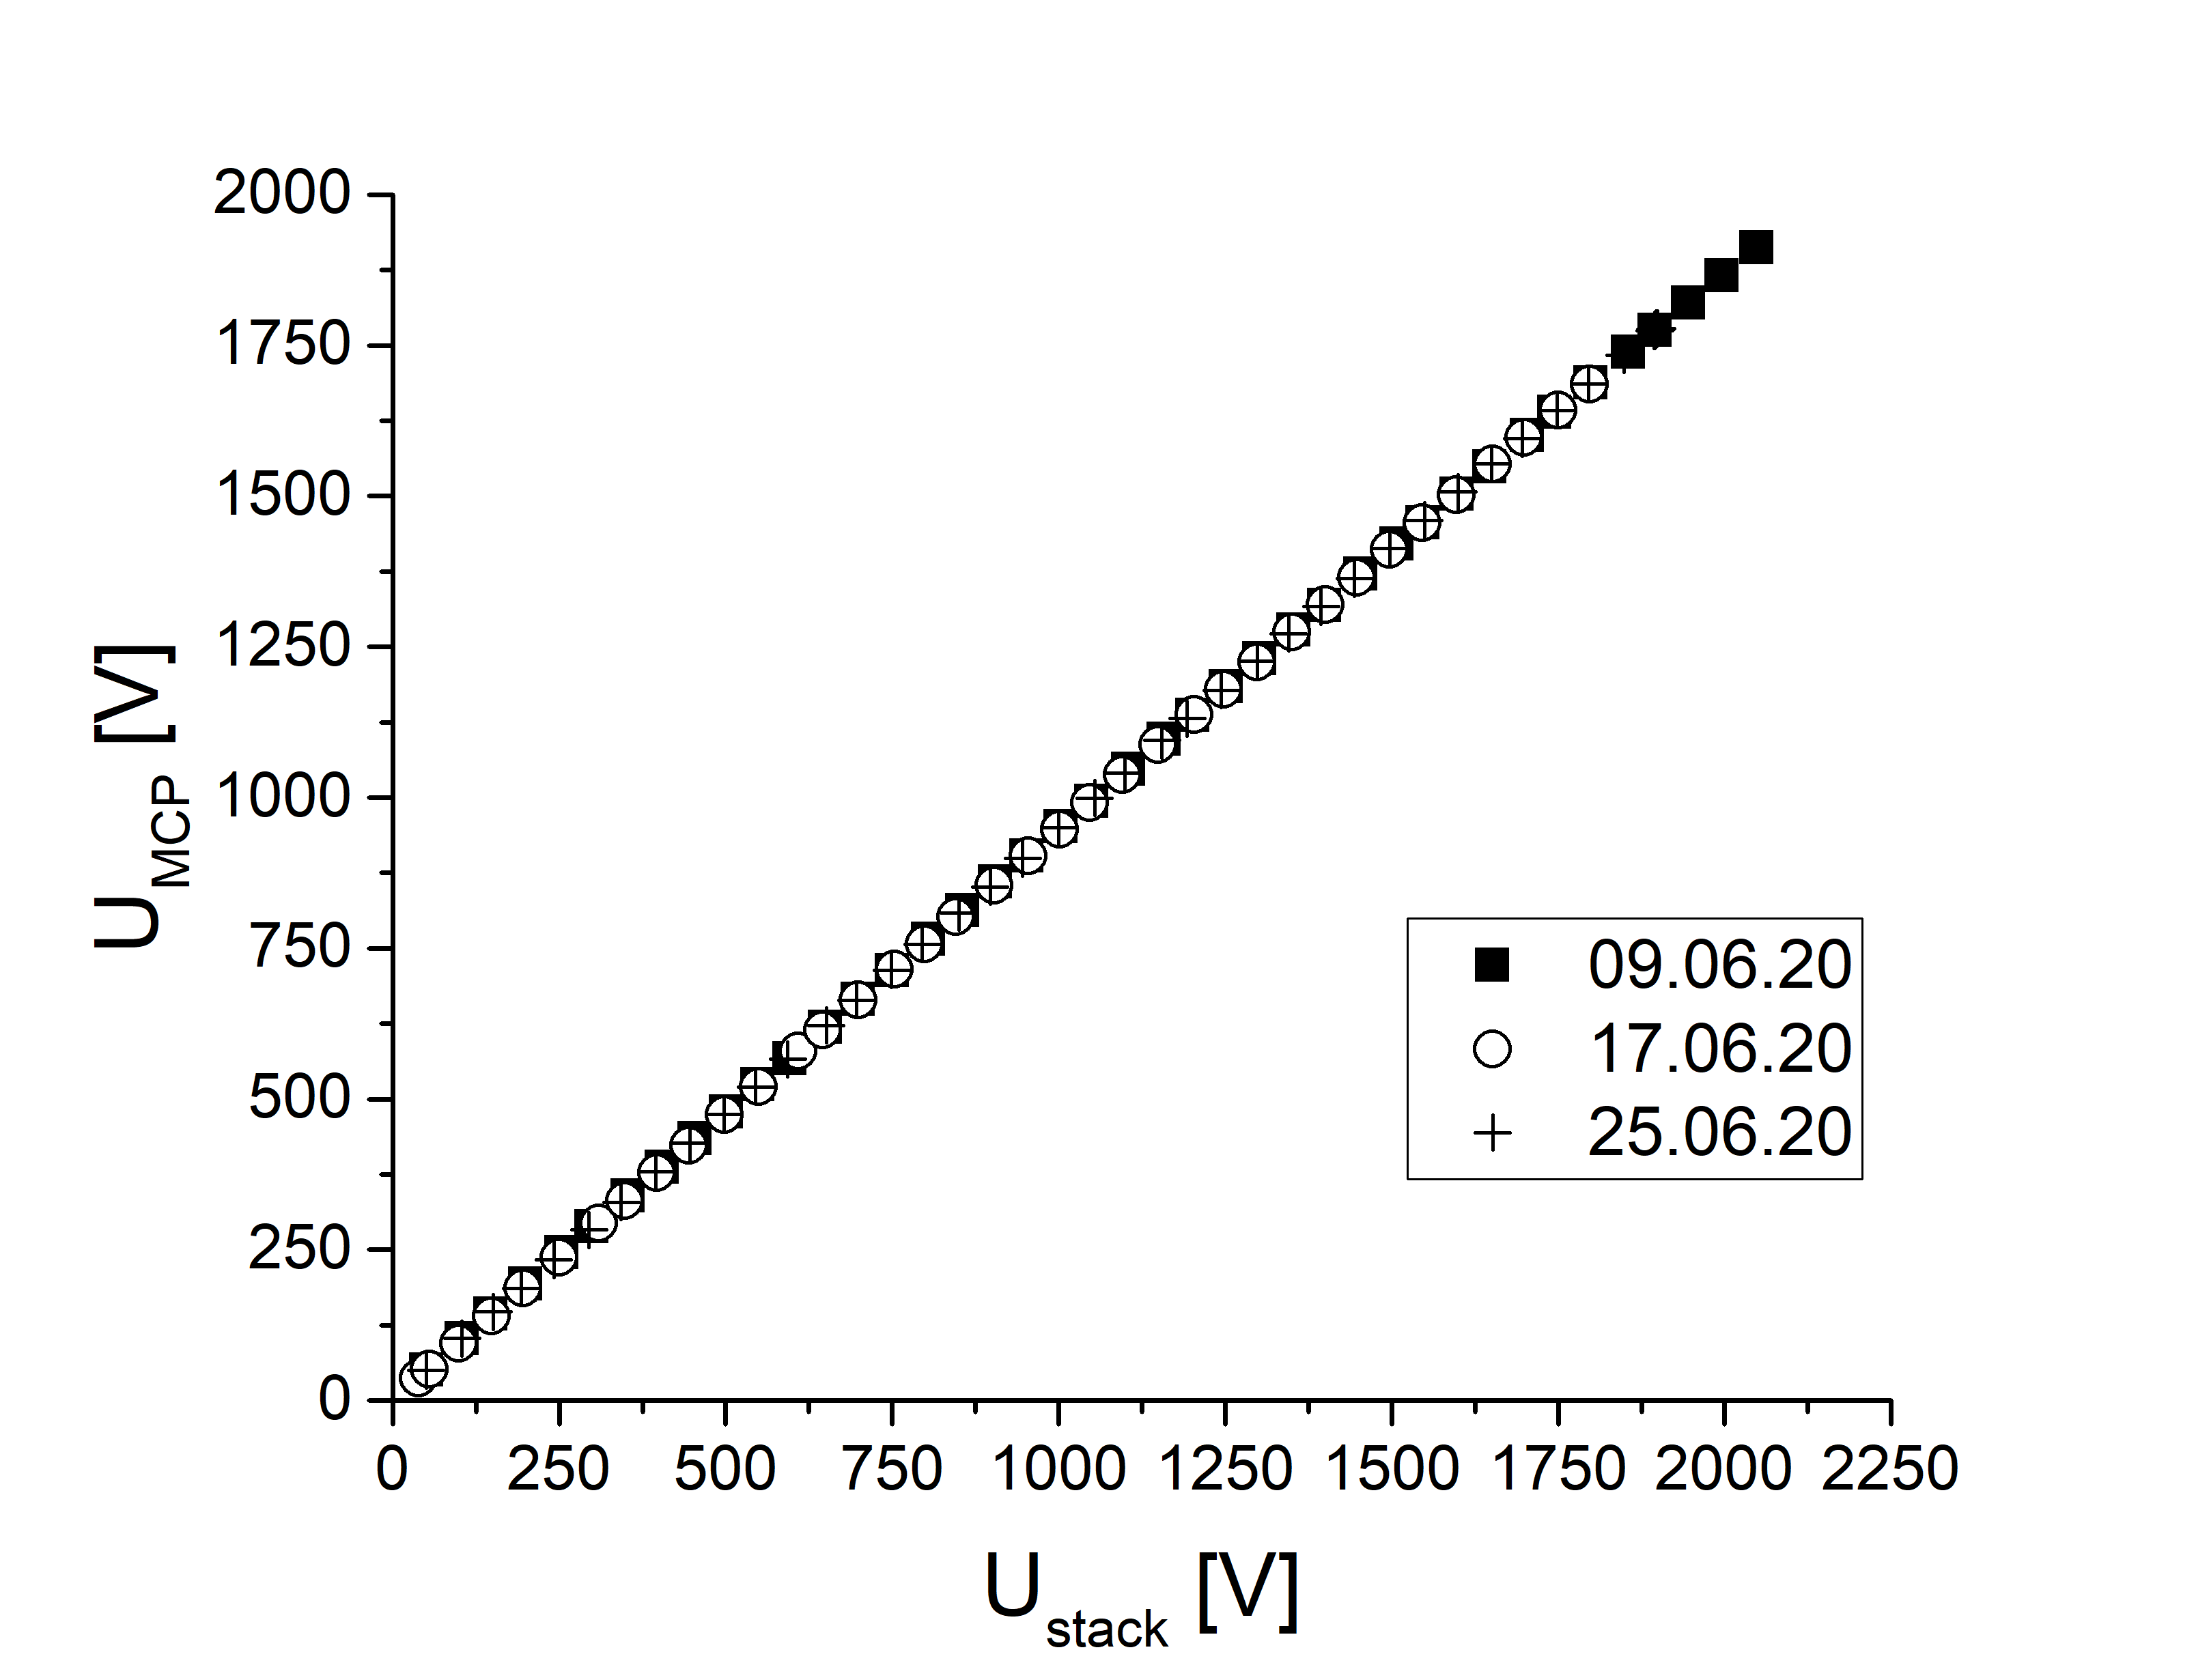
\includegraphics[width=.8\textwidth]{Experiments/PFM_UstackUmccp_TimeEvol.png}
		\caption{MCP voltage (U\textsubscript{MCP}) as a function of the voltage applied between the MCP front and the anode (U\textsubscript{stack}) for different measurement series with the PFM (black symbols) and the FS instrument (red squares) with the quadratic extrapolation.}
		\label{fig:PFMUstackUmcpTimeEvol}
	\end{figure}
	from the channel walls triggering another electron avalanche. This process generates a plasma in the MCP channels destroying the channel coating. The process is stopped when the power supply is unable to provide the current and voltage to sustain the plasma. The triggered discharge leads to a signal reduction of about 30~\% depending on at which voltage it appeared. The higher the MCP voltage was at the time of the discharge, the higher is the signal loss.\\
	Fig.~\ref{fig:MCPGainCurve4p7} shows the gain curve of detector SN~4.7 recorded when it was integrated into the NIM FS instrument. H\textsubscript{2} and H\textsubscript{2}O are part of the residual gas and \textsuperscript{84}Kr is the used test gas. The curves follow nicely the theoretical curve (see Chap.~\ref{chap:MCPGain} Eq.~\eqref{eq:MCPGain}) by fitting $U_{init}$ and $A$, where the initial energy of the released electrons $U_{init}$ is about 4~eV, which is a typical value for secondary electron emission, and the prefactor $A$ containing information about the interaction of the impinging electron with the electrons from the surface is 0.2~eV\textsuperscript{-1/2}. $\gamma$ contains information about the probability to emit the first electron for the three species and is in the range of 0.1--10.\\
	The NIM flight detector has a resistor built in between the MCPs and the anode to establish a potential difference to accelerate the electrons from the MCP exit towards the anode. The flight power supply sets the voltage between the MCP front and the anode $U_{stack}$. To determine the relation between the voltage over the MCPs $U_{MCP}$ and the stack voltage $U_{stack}$ a calibration was done with the laboratory power supplies.\\
	The resistance of the MCPs is a weak function of the applied voltage, thus a fit to the MCP voltage of the form
	\begin{equation}
		U_{MCP} = a\cdot U_{stack}^2 + b\cdot U_{stack}
		\label{eq:StackMCPCalib}
	\end{equation}
	was necessary.
	\begin{table}[h!] % Fit params of Calibration. % Old values: Uinit 6 eV, A = 0.3 eV
		\begin{center}
			\begin{tabular}{c|c|c|}
				& PFM	& FS\\ \hline
				a	& $(-1.25 \pm 0.05)\cdot10^{-5}$ & $(-1.54 \pm 0.05)\cdot10^{-5}$ \\
				b 	& $0.96 \pm 0.001$	& $0.96 \pm 0.001$\\
			\end{tabular}
		\end{center}
		\caption{Fit parameters of the quadratic interpolation (Eq.~\eqref{eq:StackMCPCalib}) for the calibration of the MCP voltage of the PFM and the FS detector.}
		\label{tab:UstackUmcpFitParams}
	\end{table}
	Moreover, this fit allows for the extrapolation to higher $U_{stack}$ values that have not been tested. Fig.~\ref{fig:PFMUstackUmcpTimeEvol} shows the results of that calibration for the PFM and the FS detector with an extrapolation up to 2.4~kV for the MCP voltage. 2.4~kV is the upper voltage limit of the MCPs according to the manufacturer. The fit parameters for Eq.~\eqref{eq:StackMCPCalib} are given in Table~\ref{tab:UstackUmcpFitParams}. The MCPs in the two detectors have similar resistances, which is the reason why the measurement data of the two detectors overlap. For the PFM detector, a longer measurement campaign was done to characterise the PFM instrument (Chap.~\ref{sec:paper}). During that campaign, this curve was recorded frequently every time the instrument was turned on. The resistance did not change significantly during the short time of the measurement campaign.
	
	
	% Measuring settings. Turn the drift voltage up to -2.5 kV and then slowly increase the anode voltage to the value you want to measure. The gain is calculated with the software by doing a Simpson 3/8 integration of the peak = Q.

		
%---------------------------------------------------------------------------------------------	
	\subsection{Instrument performance tests}
		This chapter shows performance results of the NIM PFM and the NIM FS instrument. Most results were conducted when the two instruments were operated with laboratory electronics because there was only very limited time to calibrate the two instruments as whole units.
		
		\subsubsection{Proto Flight Model}\label{sec:paper}
		\clearpage
		\newpage
		\thispagestyle{empty}
		\null
		\newpage
		
		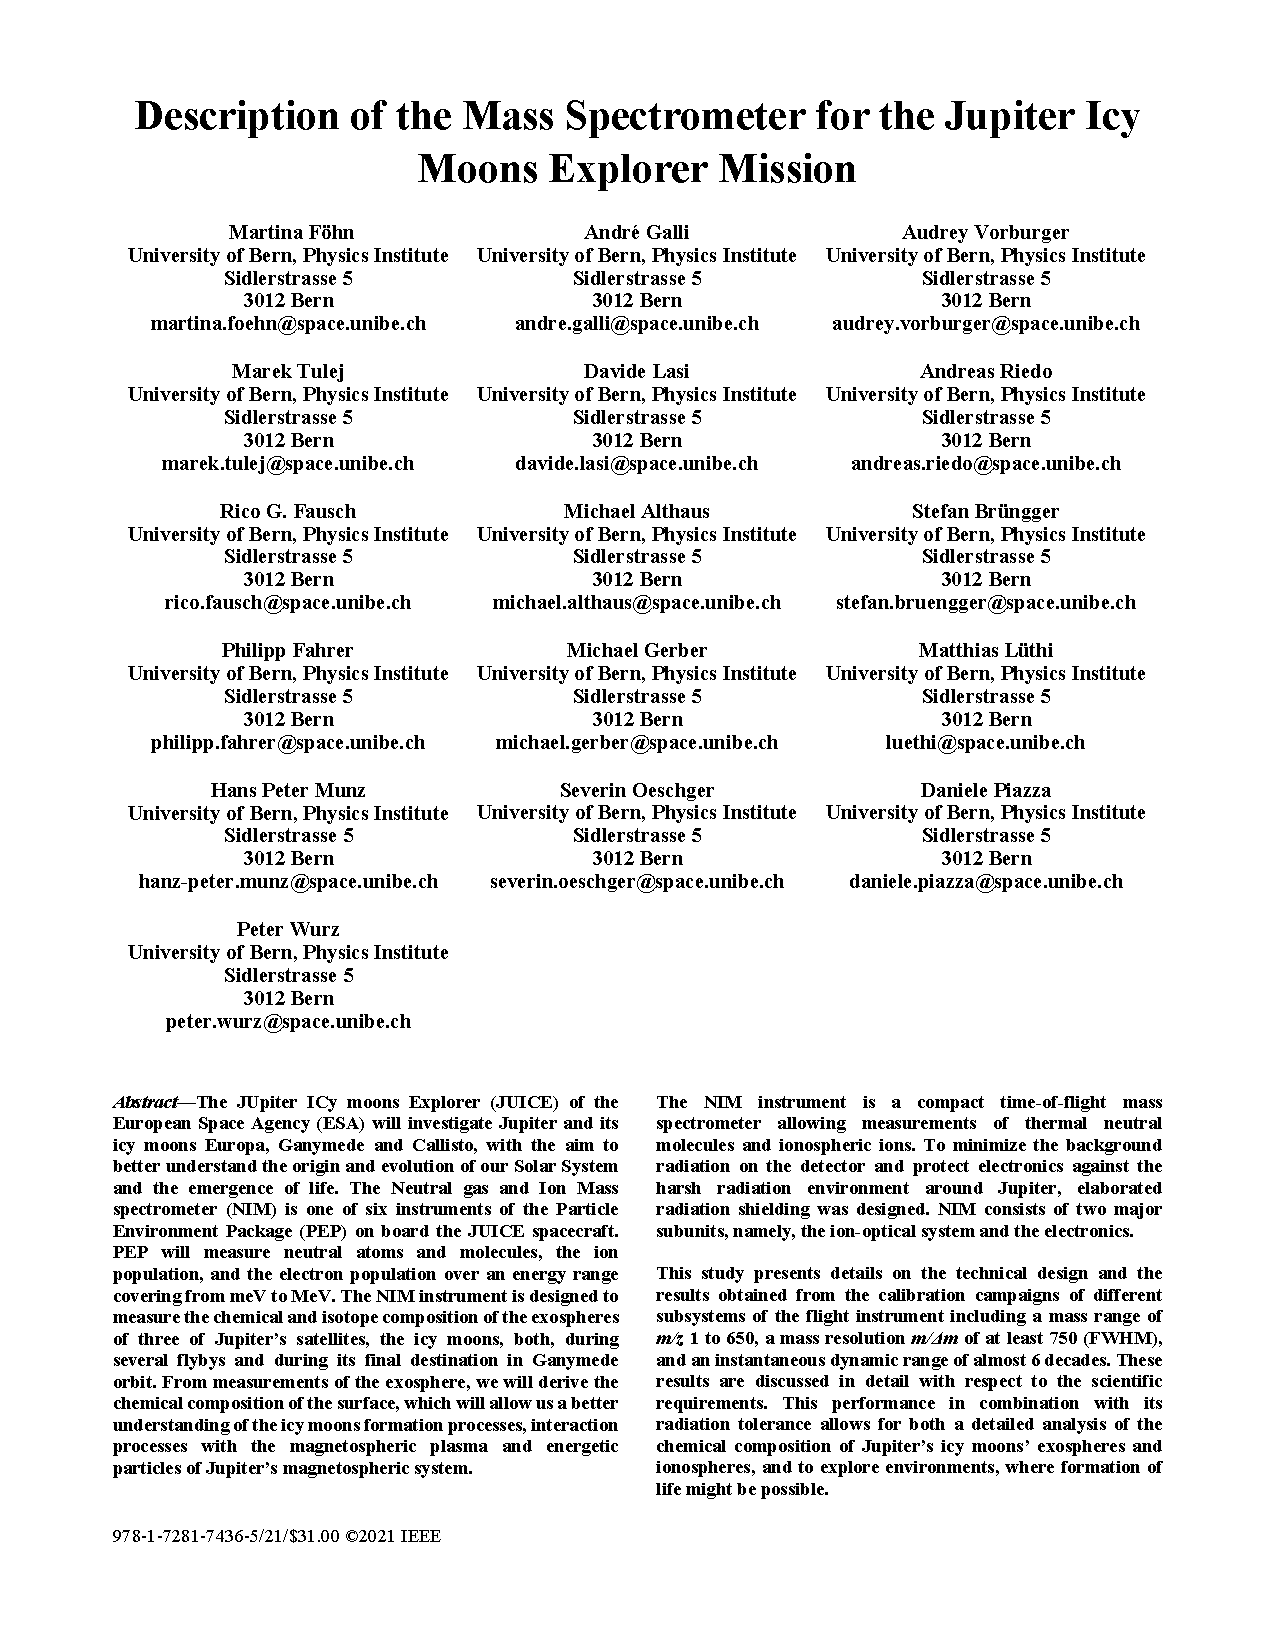
\includepdf[pages={1-}]{Foehn2021_IEEE.pdf}
		\newpage
		
%----------------------------------------------------------------------------------------------------		
		\subsubsection{Flight Spare}\label{chap:FSCalib}
		\textbf{Ion Storage}\\
		Ion storage is very crucial for a time of flight mass spectrometer because every ion generated outside of the extraction pulse interval and not stored in the ionisation region is lost. Moreover, it can generate additional electrical noise on the detector signal line because these ions would arrive at an arbitrary time at the detector, with respect to the extraction pulse. In this test the ion storage capability of the ion source was analysed for thermal and neutral mode for hydrogen and krypton with velocities of 2~km/s and 4~km/s. The electron emission current was varied from 20 to 600~\si{\micro\ampere}.\\
		Ion storage of positive ions in x- and y- direction is supported by the negative space charge potential generated by the electron beam (see Chap.~\ref{chap:TheoIonStor}). Two ring electrodes, with a positive voltage applied, generate a positive potential ring to trap generated ions in y- and z- direction (Fig.~\ref{fig:ExpFSFlightSenIonStorIS}). For emission currents from 20 to 600~\si{\micro\ampere} according to Eq.~\eqref{eq:elPotIem} the negative potential in the centre of the electron beam is --0.1 to --3.0~V. Fig.~\ref{fig:ExpFSFlightSenIonStor}, left panel shows the ion storage behaviour of the ion source of hydrogen and the right panel shows the ion storage behaviour of krypton. In case of no ion storage, the relationship between the electron emission current I\textsubscript{em} and the signal intensity is linear because then only ions would be extracted that are generated during the time when the extraction pulse is applied on the extraction grid. In case of ion storage there is a about a quadratic relationship between I\textsubscript{em} and the signal intensity.\\
		When measuring with the thermal mode, the particles are slowed down in the antechamber until they have energies in the range of 26~meV~$\widehat{=}$~300~K and are therefore easy to trap in the potential field. When measuring with the neutral mode, particles enter the ionisation region directly. The kinetic energy of hydrogen for velocities between 2~--~4~km/s is 0.07~--~0.27~eV. Therefore, hydrogen can be trapped in the potential well generated by an electron beam with an emission current higher than 20~$\mu$A.\\
		\begin{figure}[H]
			\centering
			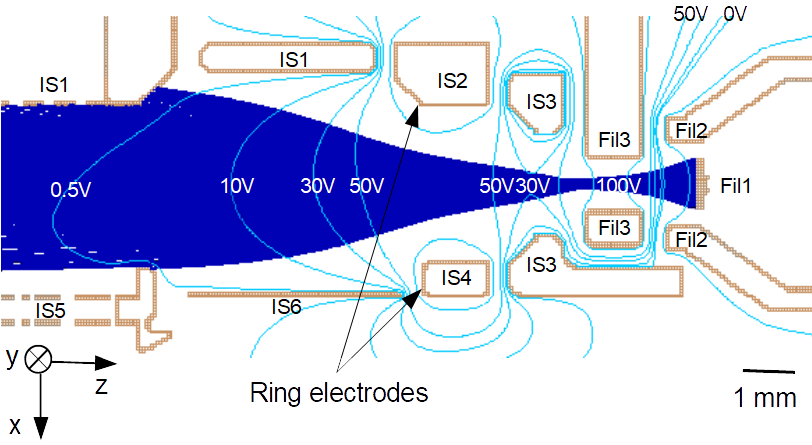
\includegraphics[width = 0.7\textwidth]{Experiments/FiL_IS_elBeam_Storage.png}
			\caption{Ion storage source with sample voltage set applied to the electrodes. In light blue are the potential lines and in dark blue are the calculated trajectories of the electron beam.}
			\label{fig:ExpFSFlightSenIonStorIS}
		\end{figure}
		\begin{figure}[H]
			\begin{subfigure}{0.5\textwidth}
				\centering
				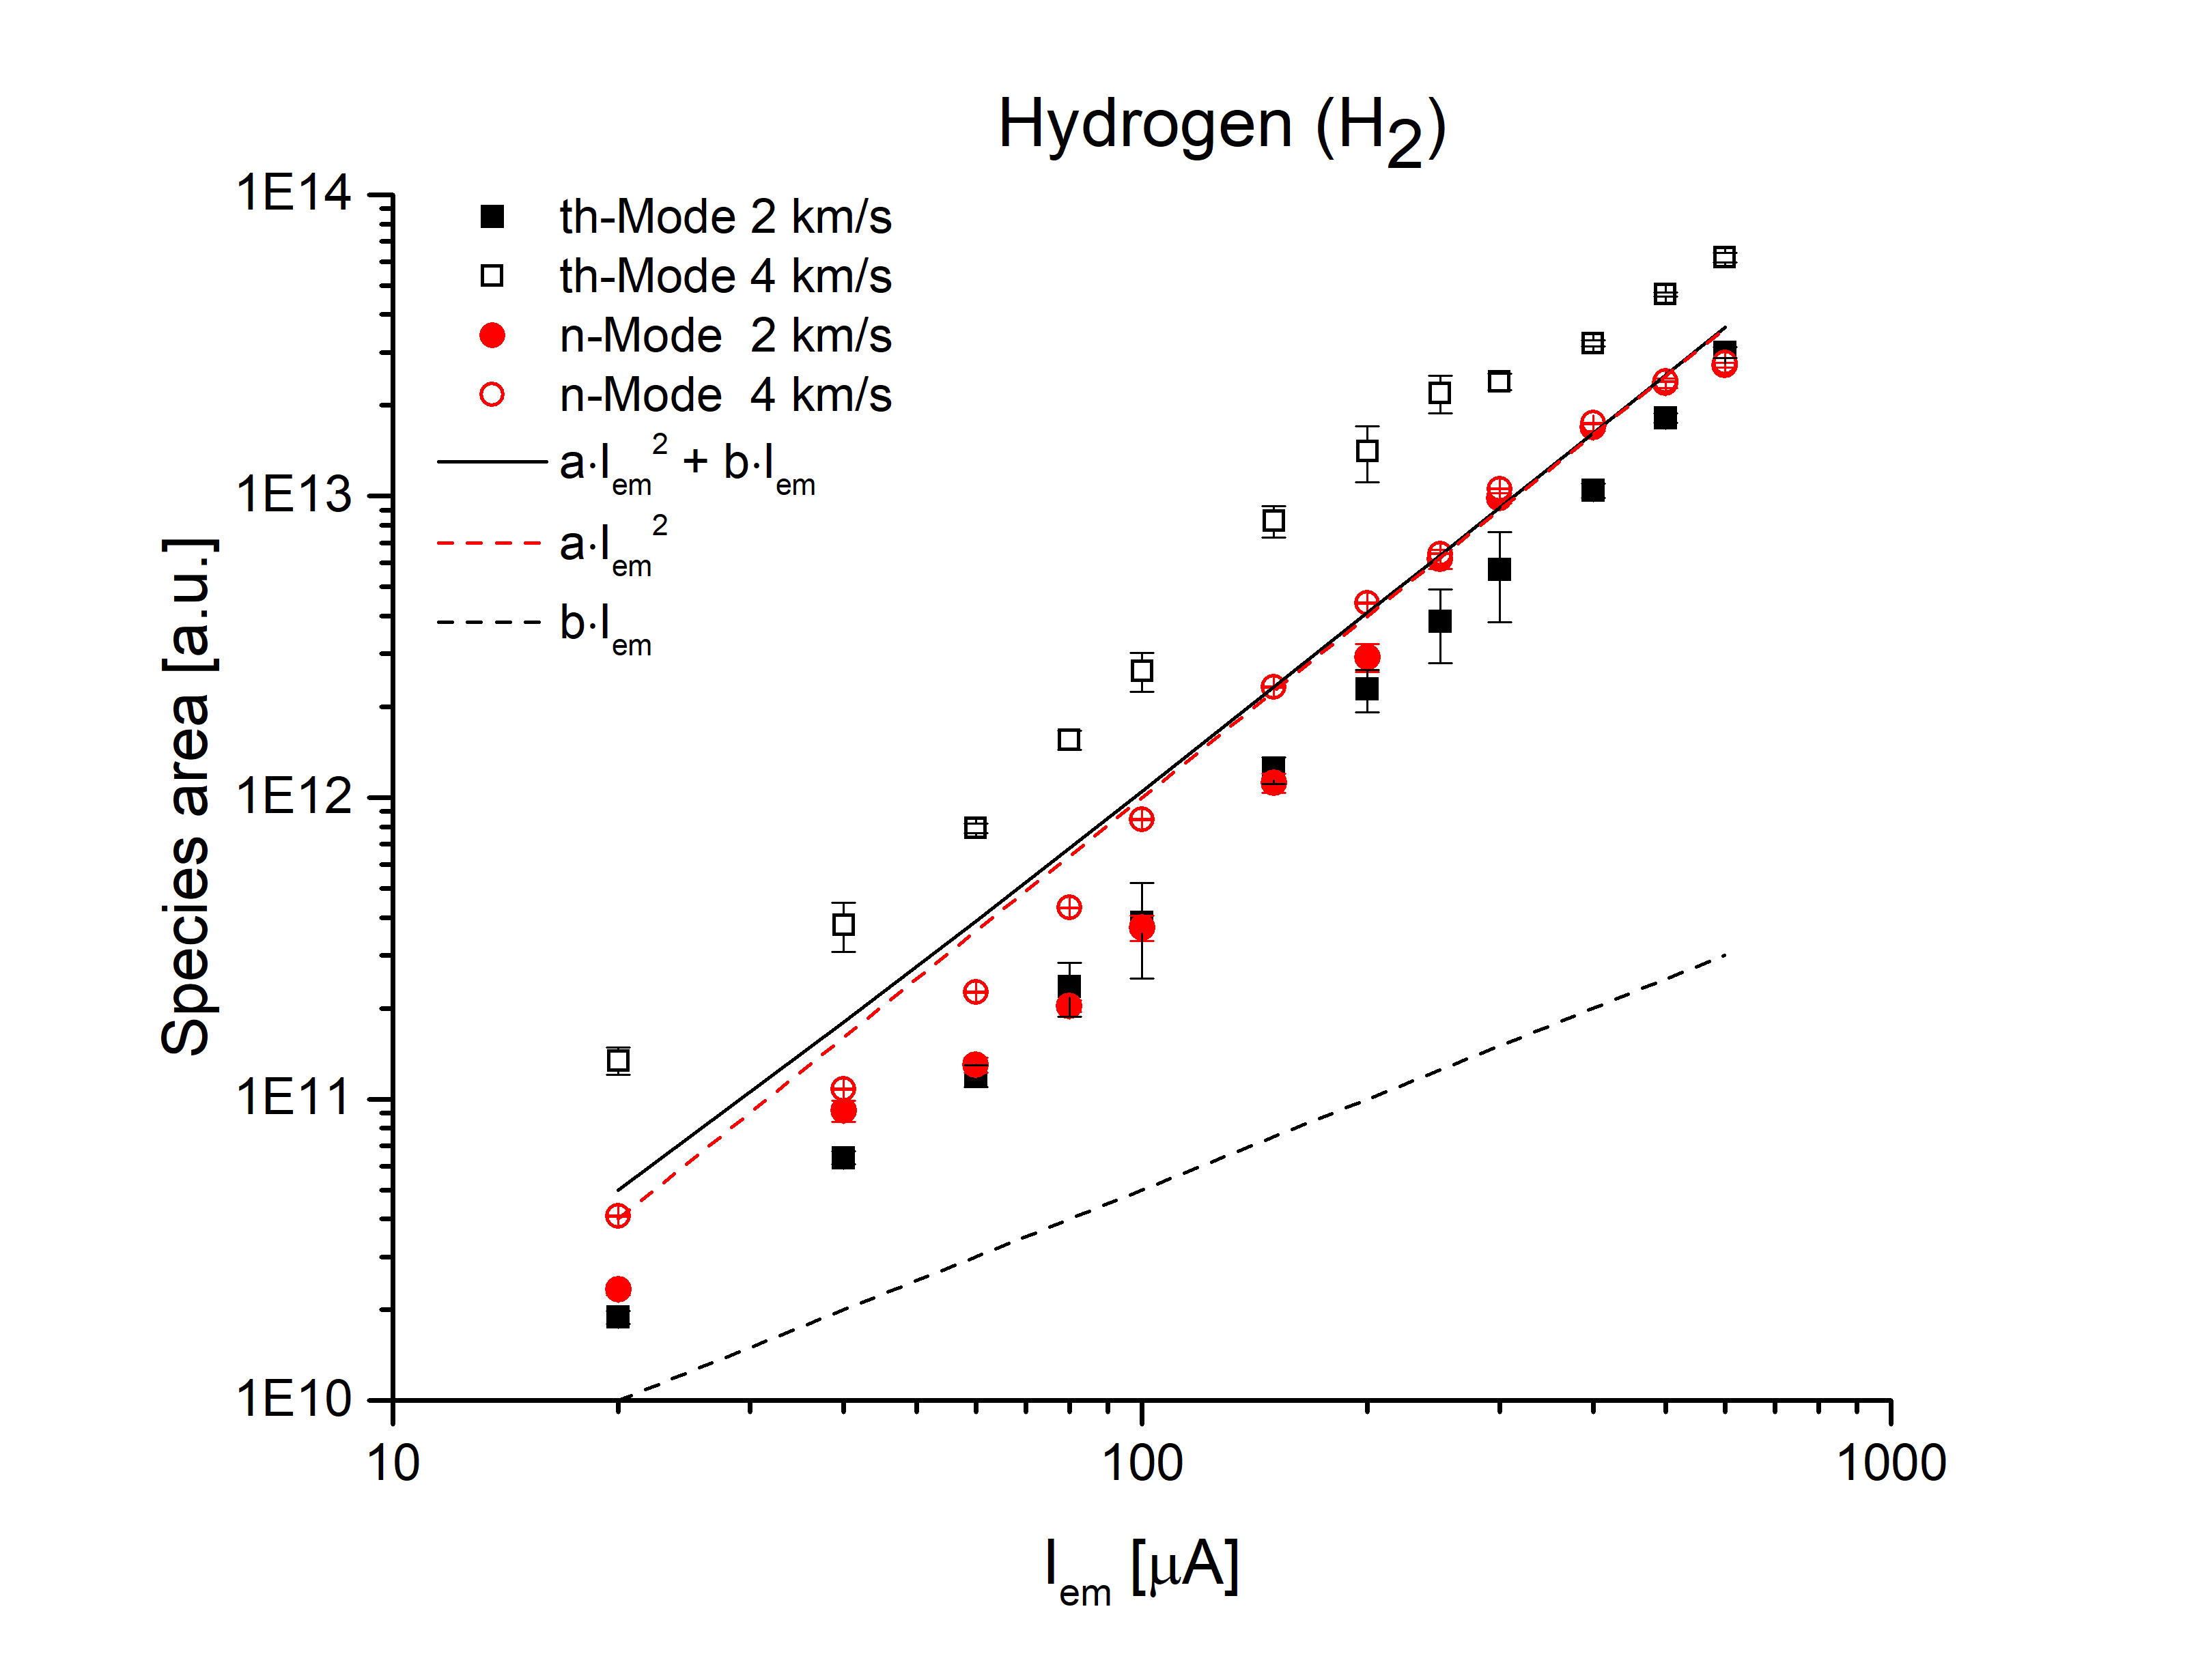
\includegraphics[width = \textwidth]{Experiments/FSLabIonStorageH2.png}
			\end{subfigure}
			\begin{subfigure}{0.5\textwidth}
				\centering
				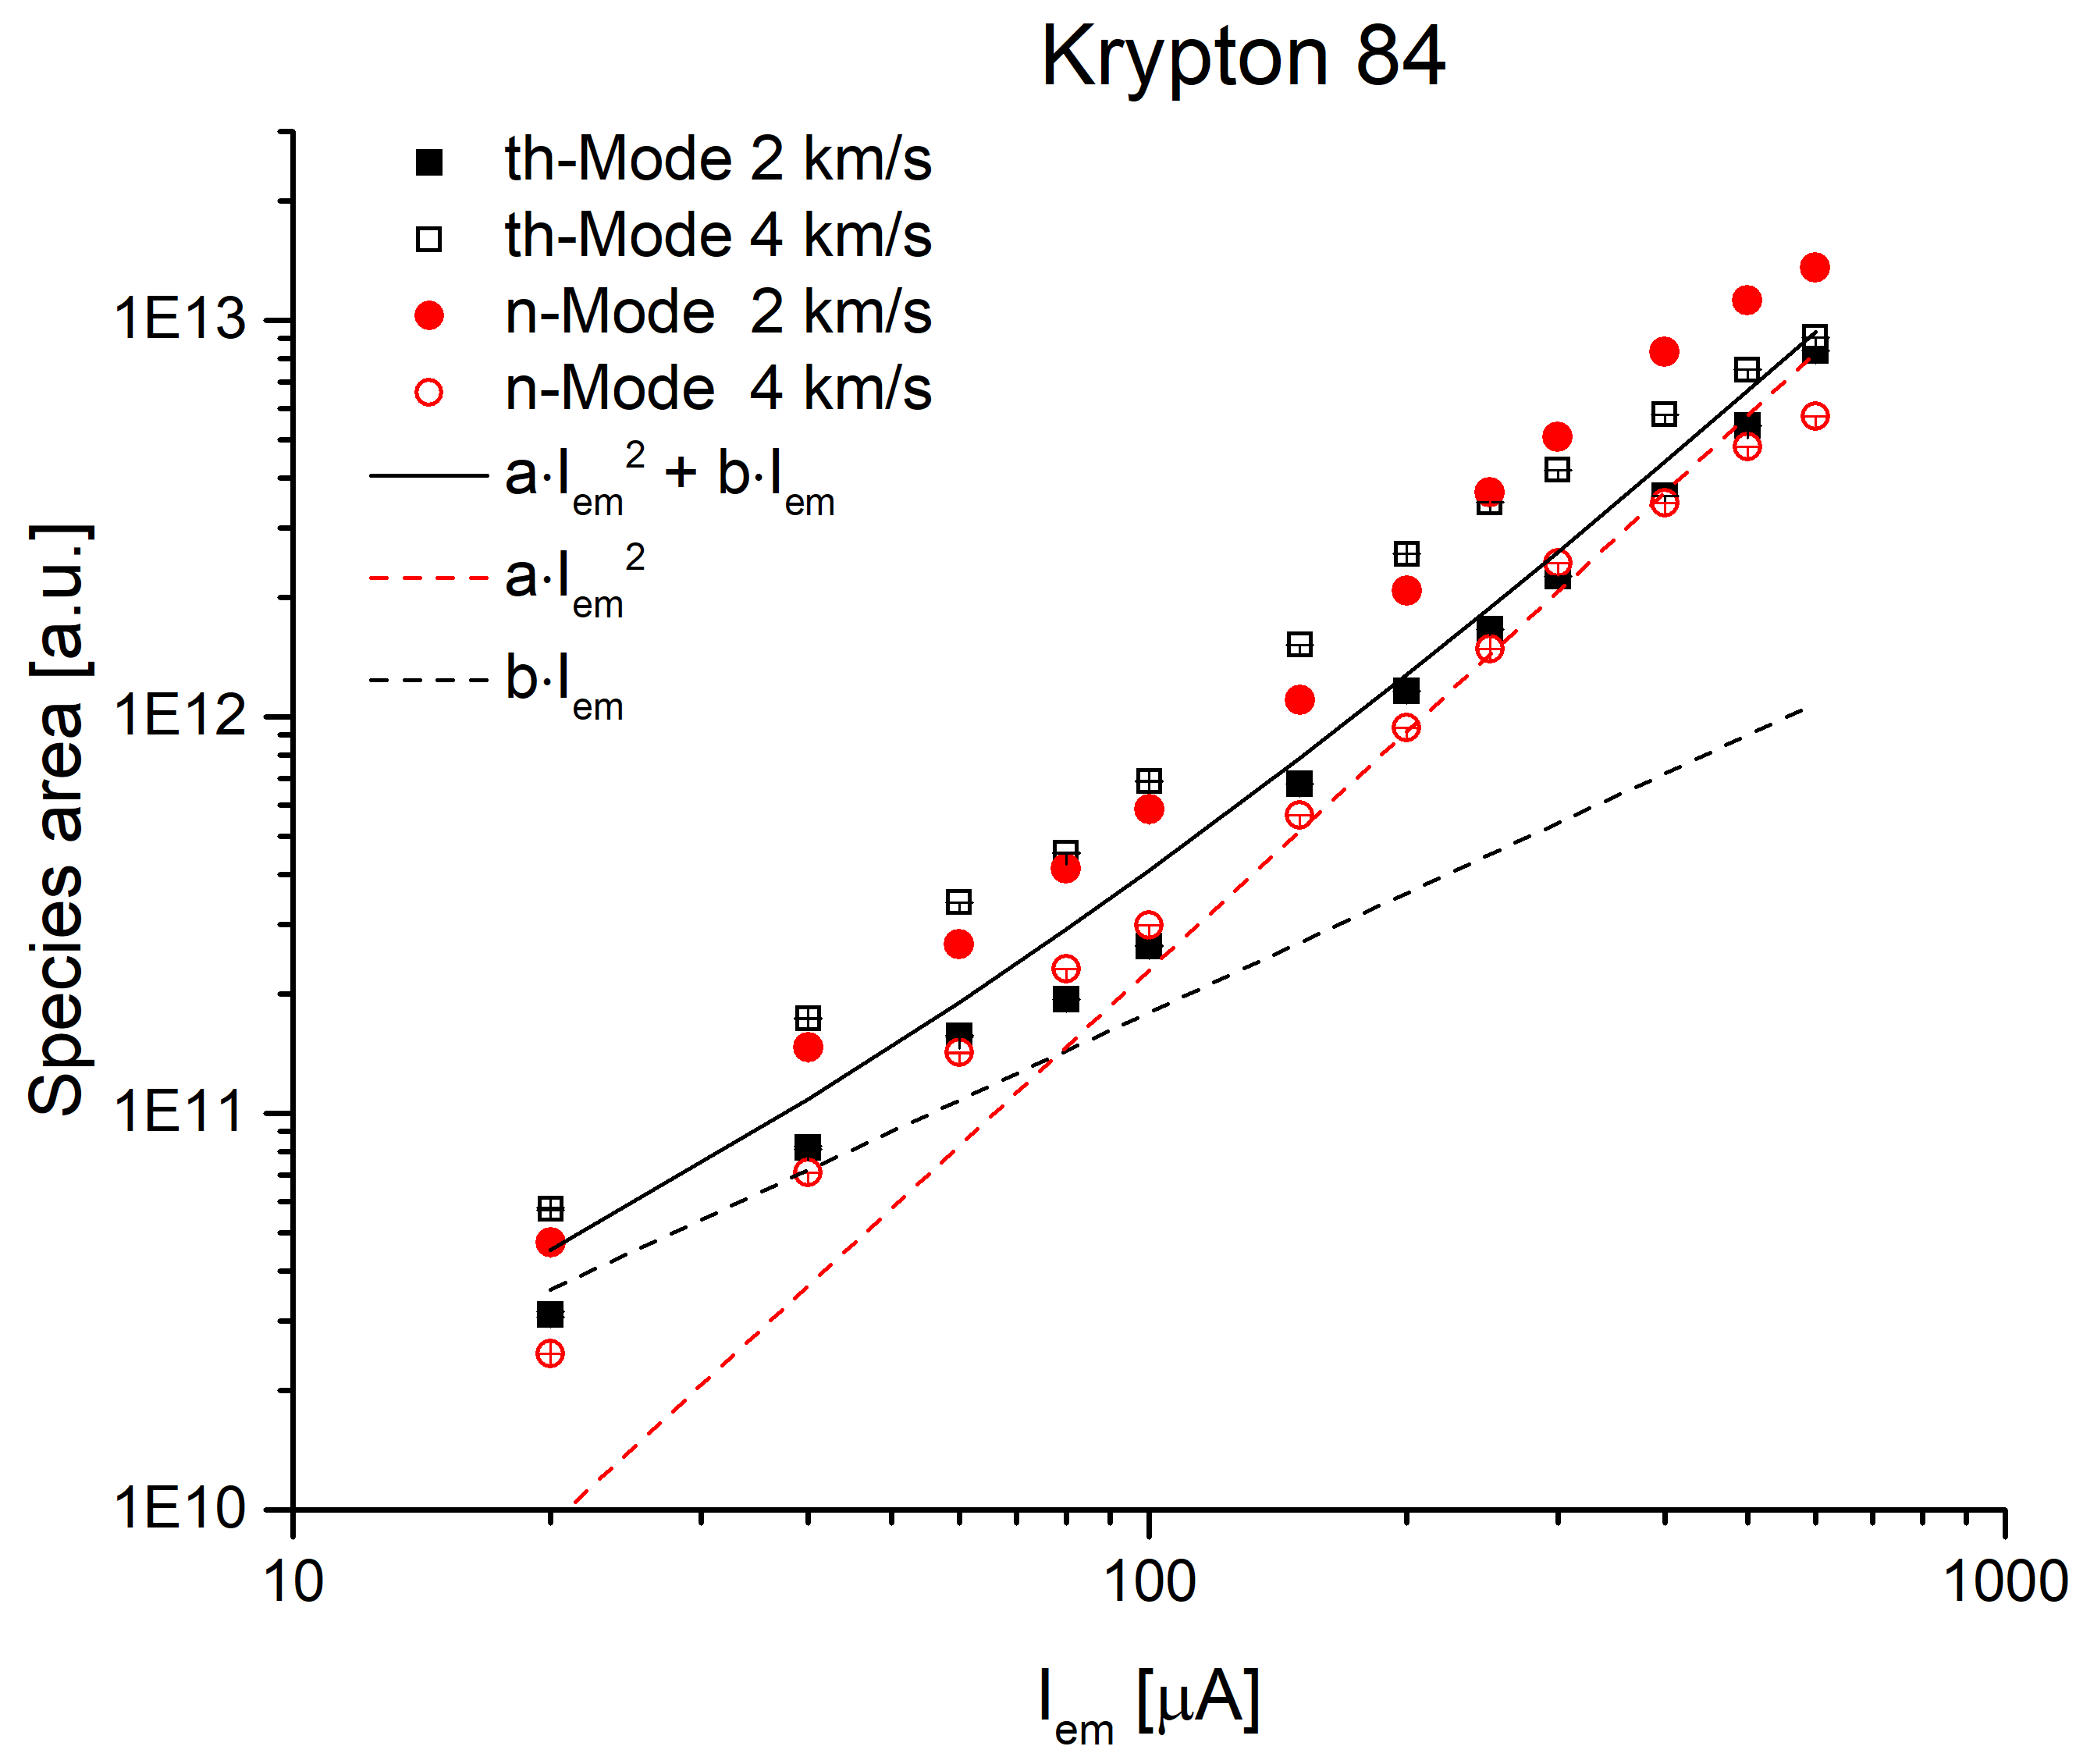
\includegraphics[width = \textwidth]{Experiments/FSLabIonStorageKr84.png}
			\end{subfigure}
			\caption{Ion storage measurements performed with the NIM  flight spare ion-optical system operated with laboratory electronics for a neutral gas beam  containing H\textsubscript{2} and \textsuperscript{84}Kr for two different gas velocities.}
			\label{fig:ExpFSFlightSenIonStor}
		\end{figure}
		The kinetic energy of \textsuperscript{84}Kr for the same velocities is 2.8~--~11.2~eV. This energy exceeds the potential of the centre of the electron beam and the ions are therefore more difficult to trap with only the electron beam. The ions are kept in the middle of the ionisation region with the positive potential ring generated by the ring electrodes. According to Fig.~\ref{fig:ExpFSFlightSenIonStor} ion storage for \textsuperscript{84}Kr starts to dominate at emission currents higher than 100~$\mu$A. In thermal mode, an increase in beam velocity leads to an increase in signal intensity due to the density enhancement effect (Chap.~\ref{subsubsec:Densenhan}). Therefore a higher signal intensity is expected in thermal mode for 4~km/s compared to 2~km/s. Like in the PFM, the FS shows a nice ion storage capability. For krypton ion storage just starts at an emission current of 100~\si{\micro\ampere} where hydrogen is stored already at lower emission currents due its lower kinetic energy at the same beam velocity.\\
		
%---------------------------------------------------------------------------------
		\textbf{Mass resolution and Signal-to-Noise Ratio}\\
		According to the requirements stated in \cite{red_book} NIM has to achieve a mass resolution $m/\Delta m$ of 500 for neutral mode and of 1000 for thermal mode. NIM is designed to measure ions and neutral molecules with masses up to 1000~u. Therefore, a mass resolution m/$\Delta$m of 1000 is required to be able to distinguish between the adjacent masses at high mass units.\\
		Fig.~\ref{fig:ExpFSFlightSenMassRes} shows two mass spectra recorded with the NIM~FS ion-optical system operated with laboratory electronics. The electron emission current was 100~$\mu$A. The mass resolution m/$\Delta$m when measuring with the neutral gas mode is 708 and 830 when measuring with the thermal mode. With this mass resolution, NIM fulfils almost the requirements regarding the mass resolution for the two measuring modes.\\
		The FS ion-optical system showed a better performance than with the PFM. The reason is that the FS ion-optical system was better optimised than the PFM. In addition, the voltages applied on some of the ion-optical lenses are extremely different between the two models (see Table~\ref{tab:voltageSets} in App.~\ref{VoltageSet}).
		\begin{figure}[h!] % SNR 600 uA emission current. Rest gas Ptot = 1.6e-9 mbar, UMCPeff = 1.8 kV. Name the gas peaks. Peaks around 200 u are not mercury because the isotopic ratio does not match the pattern.
			\begin{subfigure}{0.5\textwidth}
				\centering
				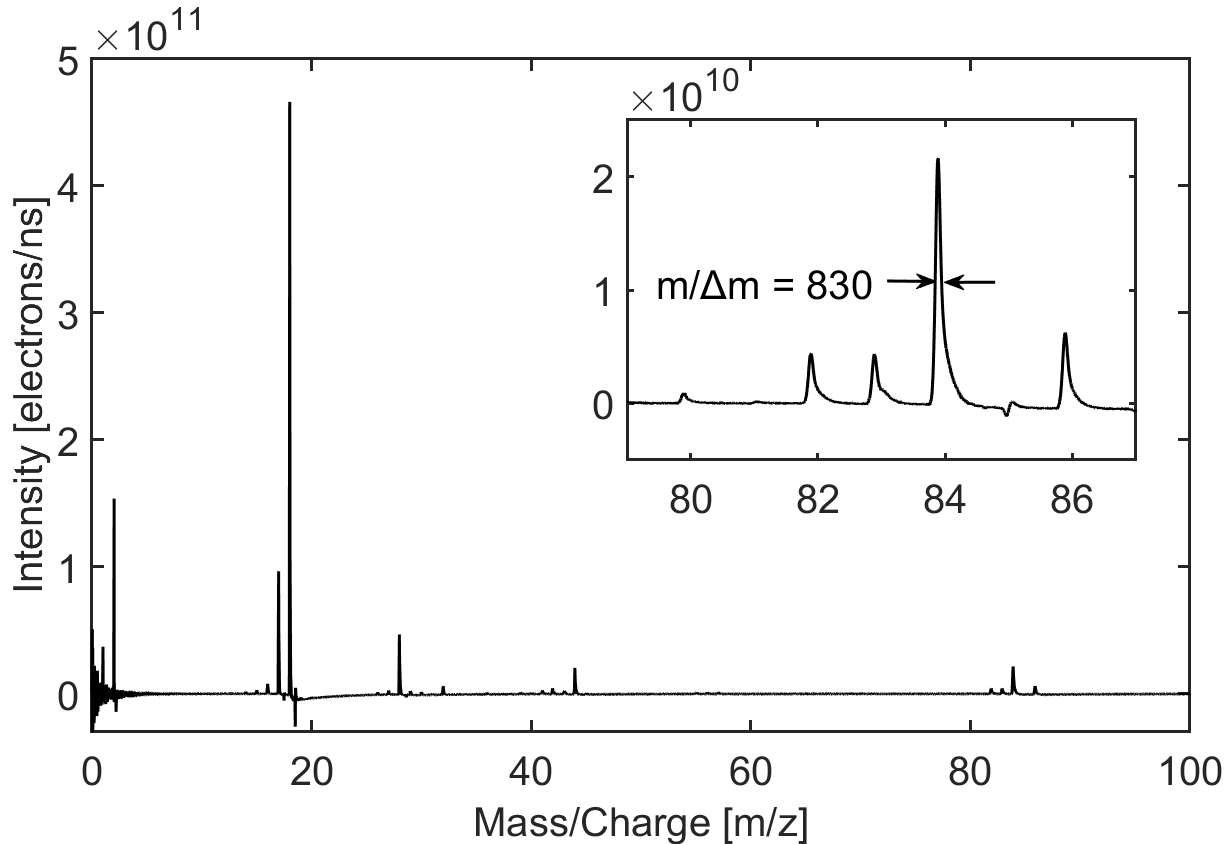
\includegraphics[width = .95\textwidth]{Experiments/FSLabthMode.png}
			\end{subfigure}
			\begin{subfigure}{0.5\textwidth}
				\centering
				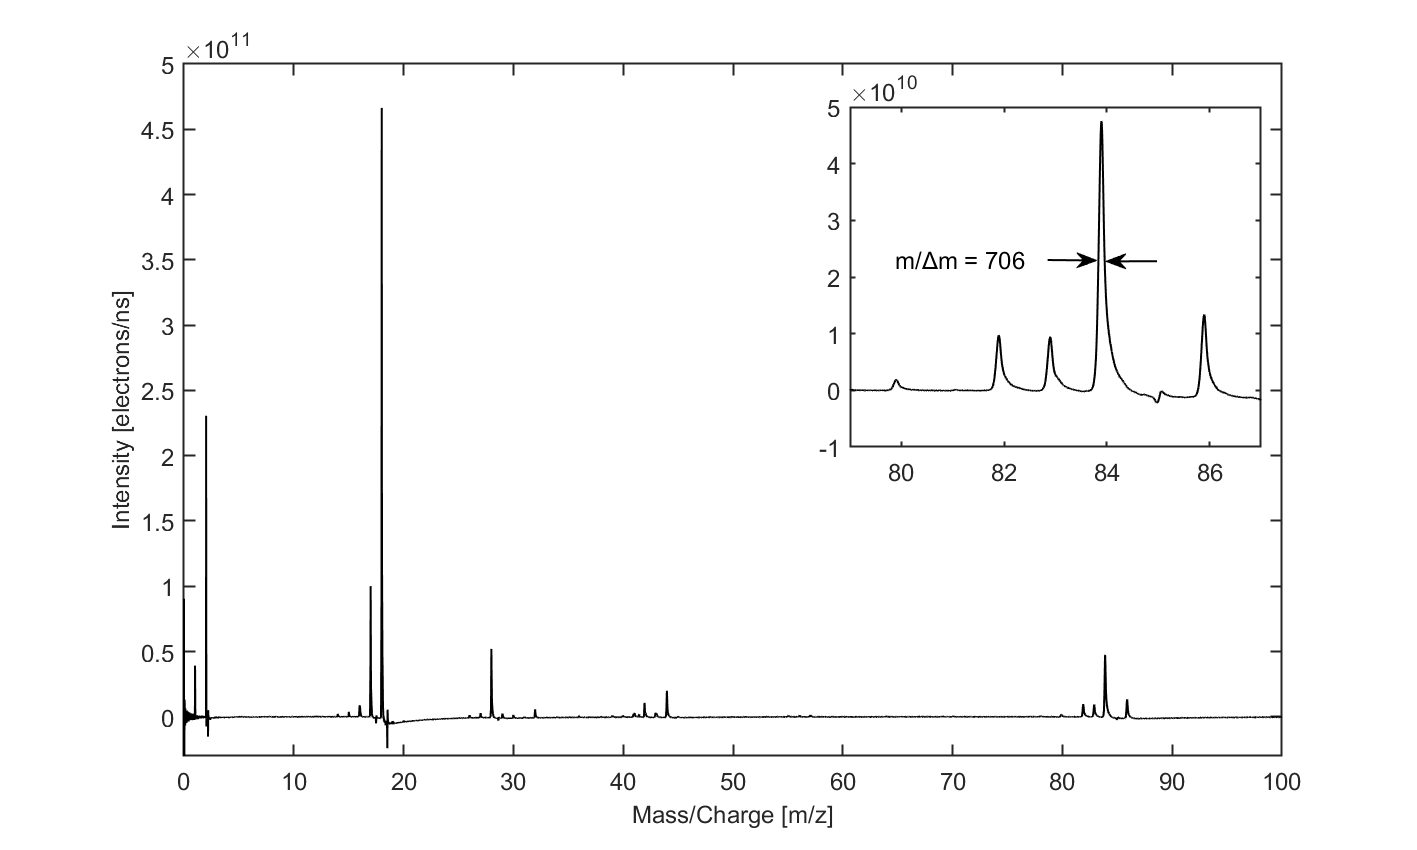
\includegraphics[width = .95\textwidth]{Experiments/FSLabnMode.png}
			\end{subfigure}
			\caption{Mass spectra measured with the NIM flight spare ion-optical system with the laboratory electronics attached. Left: thermal gas mode. Right: neutral mode.}
			\label{fig:ExpFSFlightSenMassRes}
		\end{figure}
		\begin{figure}[h] % conditions: nMode UMCP: 1950 V. P = 1.03e-8 mbar 20H2:1Kr; thMode UMCP = 1950 V. P = 6.05e-8 mbar
			\centering
			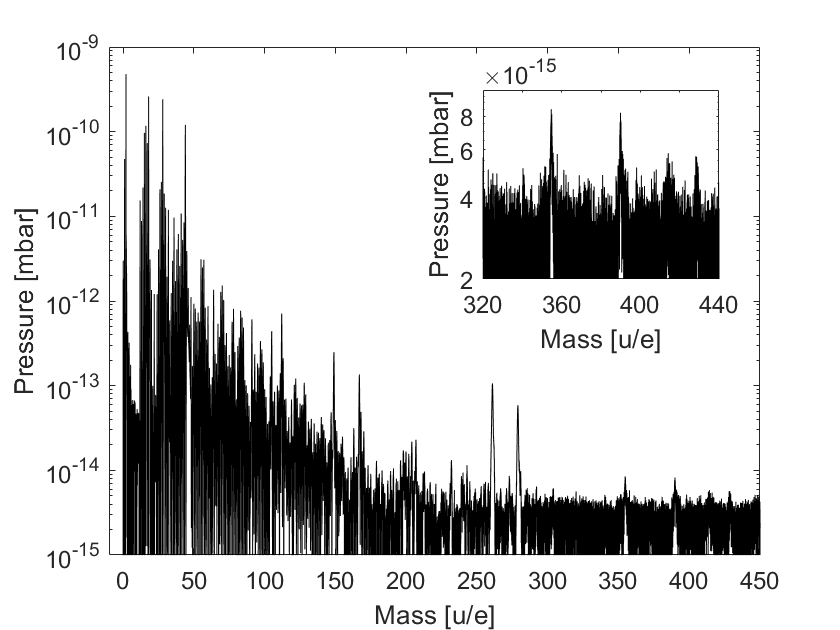
\includegraphics[width = 0.7\textwidth]{Experiments/FSLabSNRRestGasPressCal.png}
			\caption{SNR plot for the NIM flight spare ion-optical system operated with laboratory electronics. The residual gas pressure was 1.5$\cdot$10\textsuperscript{--9}~mbar.}
			\label{fig:ExpFSFlightSenSNR}
		\end{figure}
		\begin{figure}[h!]
			\begin{subfigure}{0.5\textwidth} % P Kr = 6.05e-8 mbar
				\centering
				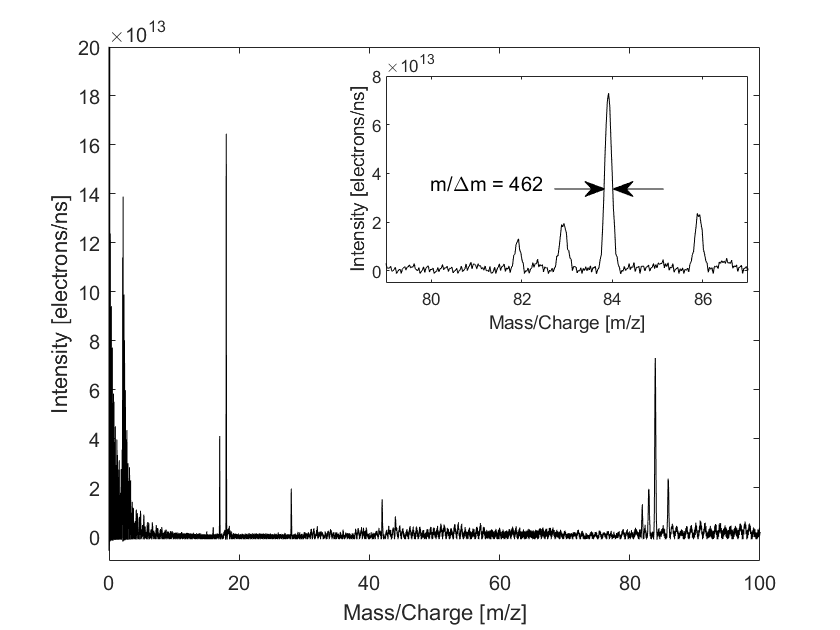
\includegraphics[width = \textwidth]{Experiments/FSthMode200uA.png}
			\end{subfigure}
			\begin{subfigure}{0.5\textwidth} % P Kr = 1.03e-8 mbar.
				\centering
				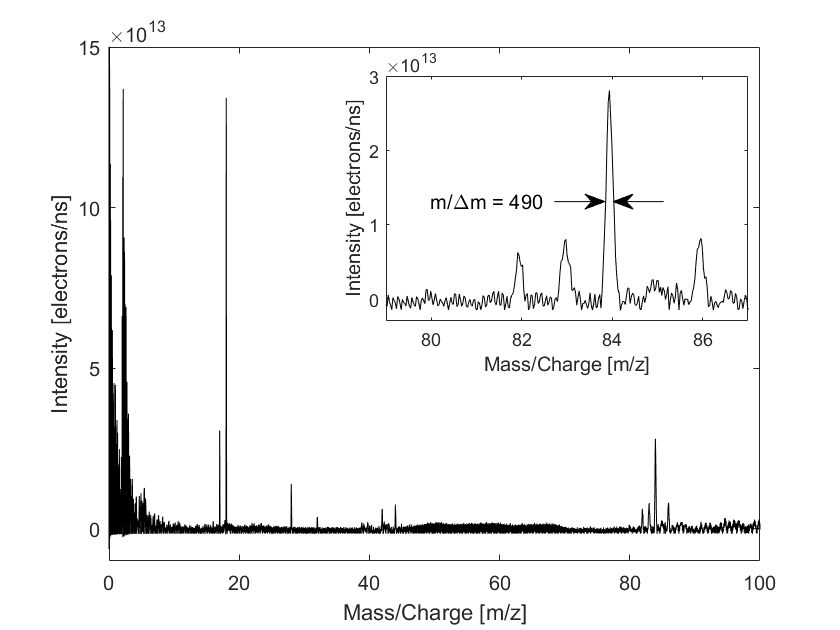
\includegraphics[width = \textwidth]{Experiments/FSnMode200uA.png}
			\end{subfigure}
			\caption{Mass spectra measured with the NIM flight spare instrument with the flight electronics attached. Filament emission current was 200~$\mu$A. Left: thermal gas mode. Right: neutral mode.}
			\label{fig:ExpFSFlightElMassRes}
		\end{figure}
		\begin{figure}[h!] % Point out at that picture that the Kr 78 isotope is clearly visible.
			\centering
			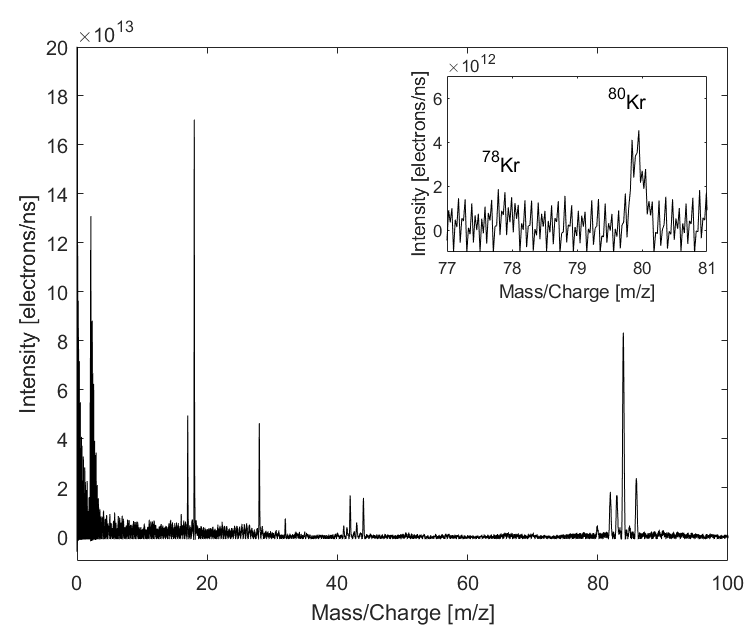
\includegraphics[width = 0.6\textwidth]{Experiments/FS_thMode300uA.png}
			\caption{Mass spectrum measured with the flight spare instrument with the flight electronics attached with a filament emission current of 300~$\mu$A.}
			\label{fig:ExpFSFlightElK78}
		\end{figure}
		\begin{figure}[h!]
			\centering
			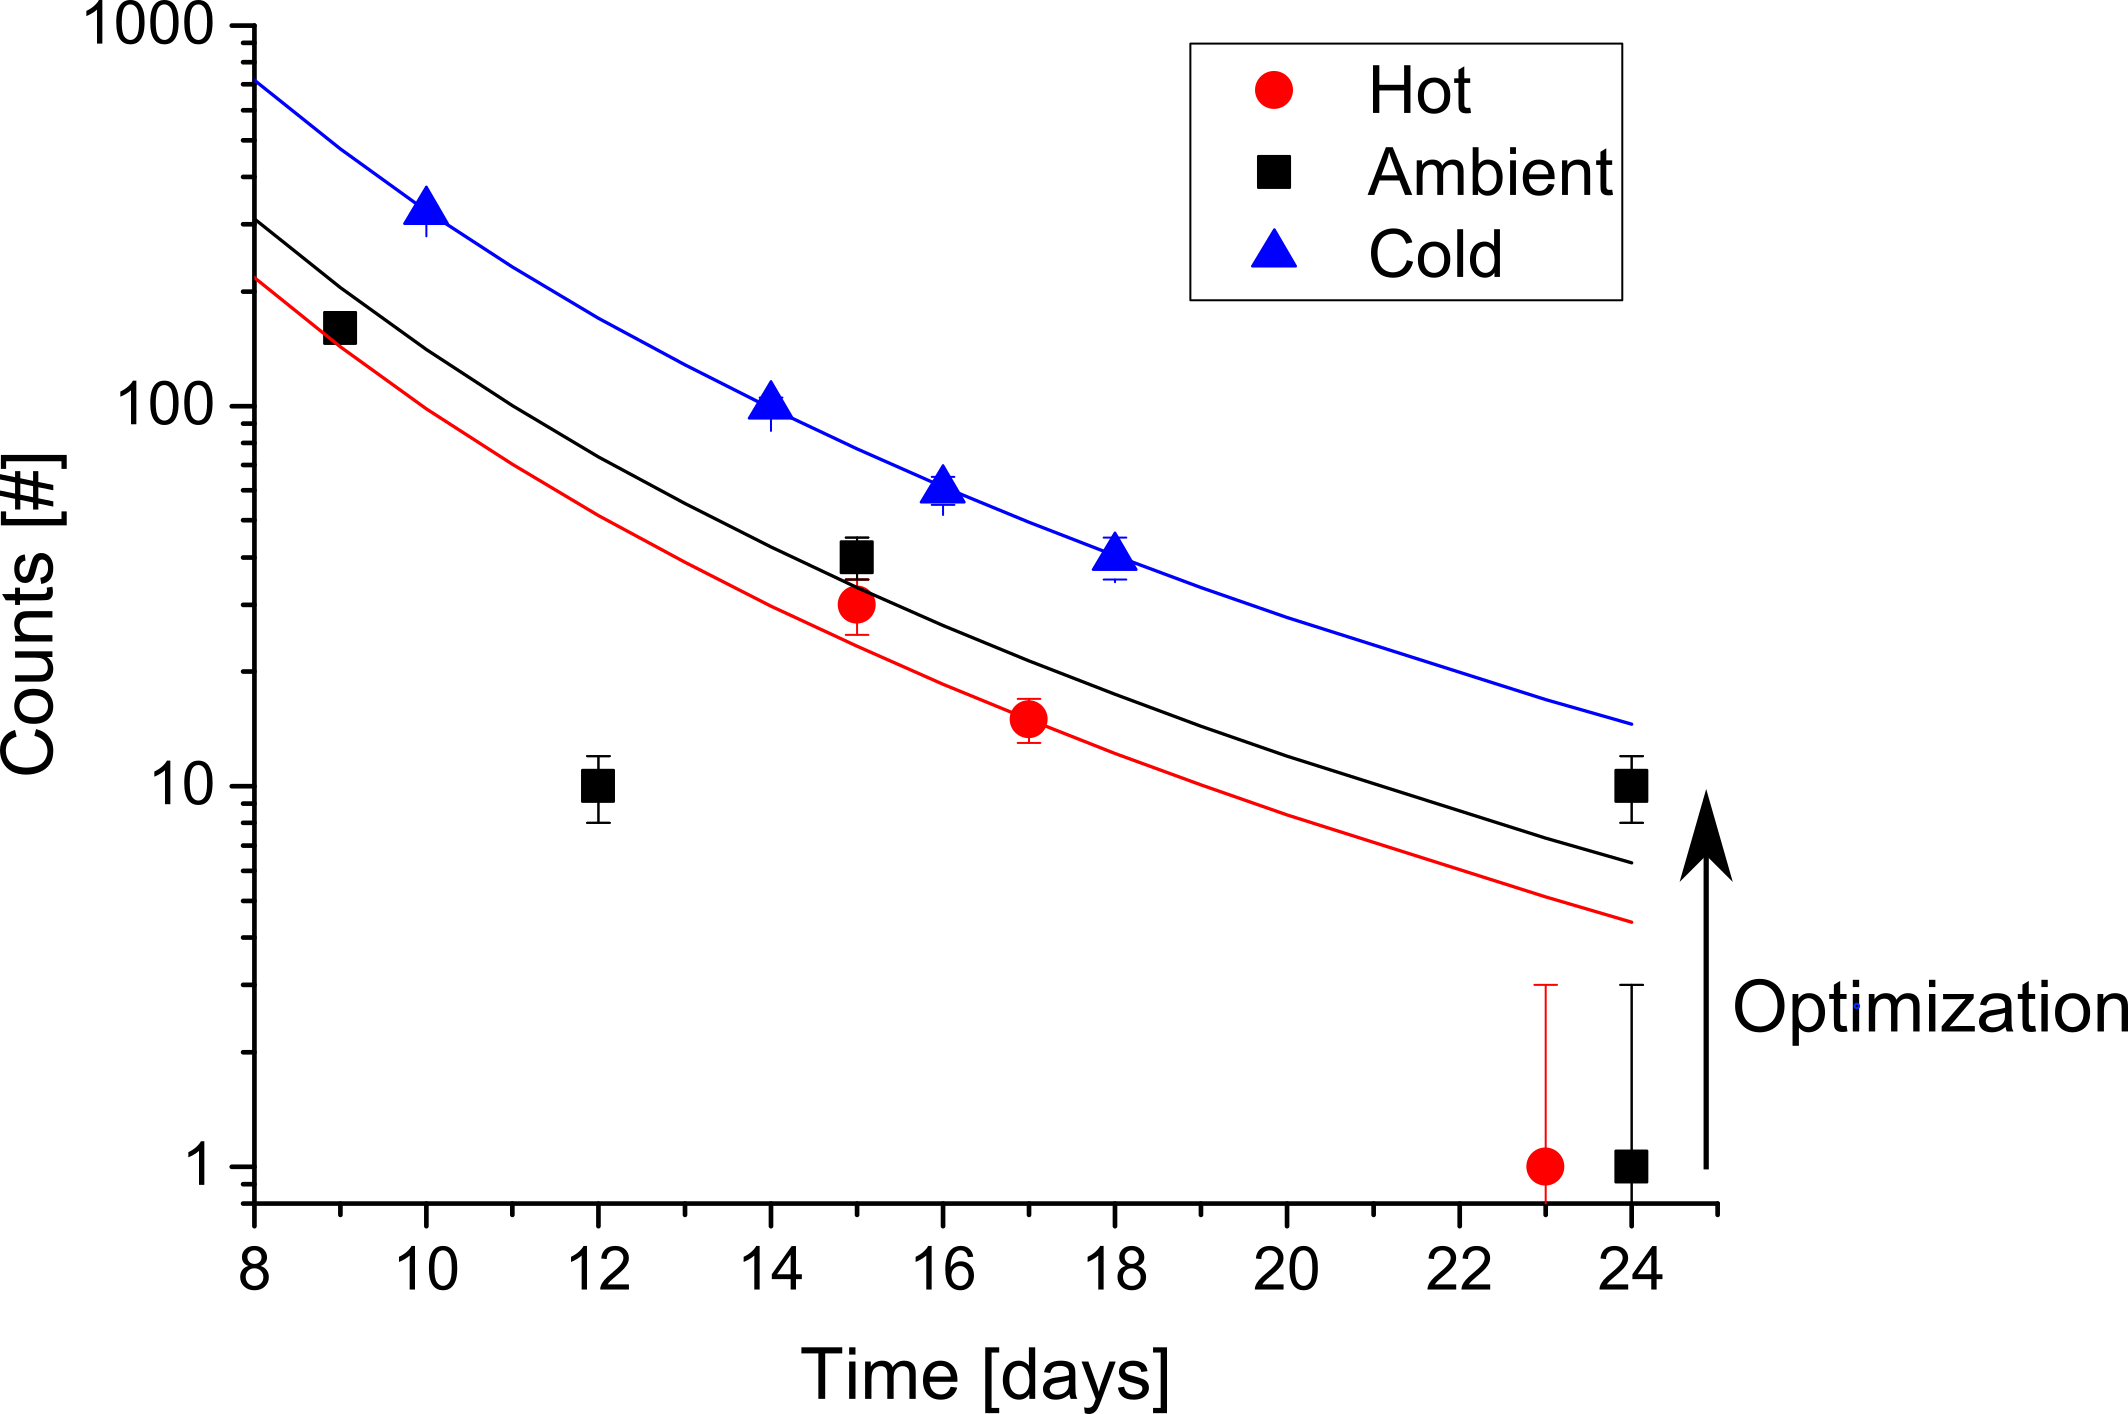
\includegraphics[width= 0.8\textwidth]{Experiments/TVT_SignalEvol.png}
			\caption{Peak height evolution of N\textsubscript{2} of the NIM FS instrument operated with flight electronics during the thermal vacuum tests.}
			\label{fig:expFSTVT}
		\end{figure}
		The biggest difference is in the applied voltage of electrode IS~1 (Fig.~\ref{fig:ExpFSFlightSenIonStorIS}). IS~1 is the electrode opposite of the extraction grids (IS~5 and IS~6) and its functions are to guide the electron beam in the ionisation region and to establish a trapping field for the ions in the ionisation region together with the other ion-optical lenses. This is a very good example on which level the ion-optics has to be optimised to reach high performance with such a compact instrument as NIM. This shows also that even when the PFM and the FS ion-optical systems are the same from the mechanical point of view, small differences in the manufacturing process have an impact on the performance of the instrument depending where they are.\\
		Fig.~\ref{fig:ExpFSFlightSenSNR} shows another mass spectrum recorded with the FS instrument when operated with laboratory electronics. The highest SNR achieved was $6\cdot10^{5}$ and therefore almost 6 decades. The mass peaks m/z 355, 390 and 429 are some oil components with water adducts originating from the turbomolecular pumps of the test facility. m/z 415 is an artefact generated by the algorithm used for background subtraction. This peak is also wider than the other surrounding mass peaks. A SNR of 6 is important to conduct optimal measurements during the flybys at Jupiter's icy moons because the experted particle densities are in the range of 10~--~10\textsuperscript{8}~cm\textsuperscript{--3} \cite{Vorburger2015, Vorburger_2018} corresponding to a partial pressure of 10\textsuperscript{--15}~--~10\textsuperscript{--8}~mbar. With a chamber pressure of 1.5$\cdot$10\textsuperscript{--9}~mbar NIM has to achieve a SNR of 6 decades to measure particles at a pressure of 10\textsuperscript{--15}~mbar.\\
		
		% FS El
		In the following section a few performance results are discussed where the NIM ion-optical system was operated with the actual flight electronics. The instrument was at that time barely optimised.\\
		Fig.~\ref{fig:ExpFSFlightElMassRes}, left panel shows a mass spectrum conducted with thermal mode and the right panel shows a spectrum recorded with the neutral mode. The electron emission current was 200~$\mu$A. The mass resolution at the current state is 490 m/$\Delta$m for neutral gas mode and 462 m/$\Delta$m for thermal mode. The mass resolution can be improved by further optimising the system as there was barely time to optimise the instrument as a whole unit. With an emission current of 300~$\mu$A the SNR is high enough to also show the \textsuperscript{78}Kr isotope, which has a natural abundance of 0.36~\% (Fig.~\ref{fig:ExpFSFlightElK78}).\\
		A lot of potential to increase the SNR lies in the analysis and removal of the noise. One part of the noise is moving depending on when the recording of the mass spectrum is started. In Fig.~\ref{fig:ExpFSFlightElMassRes}, left and right panel this noise appears between masses m/z 40 and 70. In Fig.~\ref{fig:ExpFSFlightElK78} the noise part starts right after the interference by the extraction pulse and ends at m/z 30. At the moment it is unclear what induces that noise but with a proper filter this noise can be detected and significantly reduced during data processing without affecting the mass signal peaks.\\
		Fig.~\ref{fig:expFSTVT} shows the evolution of the peak height of N\textsubscript{2} as a function of days during the thermal vacuum test campaign. During the thermal vacuum test the instruments robustness and behaviour is tested when it is under thermal stress. The iteration of the different temperature plateaus is visible in the graphic by the sequence of the different measurement points between hot, cold and ambient cases. The measuring point at day 12 is an outlier. The data clearly show a continues decrease of the signal height during operation although the used parameter set was the same for all measurements shown in the plot. The signal decline is a result of voltage drifts during the thermal cycling. When electric components are thermally cycled, thermal hysteresis effects on the electrical components can occur leading to voltage and current drifts. The readout electronics is also affected by these effects and therefore such drifts may not be noticed by the control system. Therefore, the system cannot readjust. To compensate these effects, the instrument has to be readjusted by optimising the voltages of the ion-optical lenses. The impact of the optimisation is very well visible when looking at the last data point at day 24 in the measuring series. The signal was barely visible in the noise and by a short manual optimisation of the system, a factor 10 in signal intensity was gained. With a complete optimisation recovery of the initial performance is expected. Although that is an extreme example how much can be gained by a short optimisation, it nevertheless shows the importance of having an autonomous optimisation system implemented in the flight software. The optimisation algorithm has yet to be implement. In the laboratory the optimisation can be done with the same software or manually. At the current state, the operation software is still not on a level allowing convenient manual optimisation because the flight software has higher priority to be ready before the start of the spacecraft. After the start there is only limited access to update the software on the spacecraft. The improvement of the usability of the software will be the next task in the implementation to finalise the flight software.
		
		
		
	
	
	
	